\documentclass[a4paper]{article}
\usepackage{ctex}
\usepackage{geometry}
\usepackage{amsmath}
\usepackage{ulem}
\usepackage{graphicx}
\usepackage{siunitx}
\usepackage{enumitem}
\usepackage{multirow}
\usepackage{adjustbox}
\usepackage[hidelinks]{hyperref}
\usepackage{tabularx}
\usepackage{array}
\usepackage{float}
\usepackage{tikz}
\usetikzlibrary{arrows.meta, positioning,patterns}
\newcolumntype{Y}{>{\centering\arraybackslash}X}
\usepackage[skip=8pt]{caption}

\geometry{left=2.5cm, right=2.5cm, top=2.5cm, bottom=2.5cm}
\zihao{-4}

\begin{document}

\noindent\textbf{班级：24级整合科学班} \hspace{1cm} \textbf{学号：2400017802} \hspace{1cm} \textbf{姓名：冯翊展} \hspace{1cm} \textbf{评分：}\\
\textbf{同组学生：无} \\
\textbf{实验名称：简易光谱仪的制作}   \hfill \textbf{实验日期：2025年4月25日} 

\hrule
\vspace{3mm}

\begin{enumerate}[label=\chinese*.,left=0pt]
    \item 实验目的
    \\[3mm]
    使用光栅制作简易光谱仪，观察不同类型的光源并绘制光谱图。

    \item 基本原理
    \begin{enumerate}[label=\arabic*.,left=0pt]
        \item 光栅分光原理
        \\
        由大量等宽等间距的平行狭缝构成的光学器件称为光栅，其工作原理是夫琅禾费多缝衍射。当单色光垂直照射到光栅上时，不同方向上的出射光会出现干涉增强，干涉的极大位置满足下面的光栅方程：
        $$d \sin \theta = m \lambda$$
        其中 $d$ 是光栅常数，$m$ 是衍射级数（$0,\pm1,\pm2,...$），$\theta$ 是第 $m$ 级衍射角，$\lambda$ 是入射光的波长。衍射角 $\theta$ 可以通过光栅与光屏的距离 $L$ 和 中心（零级）到 $m$ 级衍射光斑的距离 $x$计算：
        $$\tan \theta = \frac{x}{L}.$$

        \item 简易光谱仪设计
        \begin{center}
            \begin{tikzpicture}[scale=1]

            % 光源（黄色圆）
            \fill[yellow] (-3,2) circle (0.5);
            \node at (-3, 1) {光源};

            % 狭缝开口
            \draw[very thick] (-1,3) -- (-1,2.05);
            \draw[very thick] (-1,1.95) -- (-1,1);

            % 外框
            \draw[very thick] (-1,3) -- (7,3);
            \draw[very thick] (-1,1) -- (7,1);
            \draw[very thick] (7,3) -- (7,1);

            % 光栅线（两条细黑线）
            \draw[double, line width=1.2pt, double distance=0.8pt] (6,1) -- (6,3);

            % 标签
            \node at (-1,3.3) {狭缝};
            \node at (6 ,3.3) {光栅};
            \node at (7,3.3) {相机};

            \end{tikzpicture}
        \end{center}

        光谱仪主要由四个部分组成：由黑色泡沫板制成的暗室，遮去外部光源并提供黑色的背景，避免杂光干扰观察；二是狭缝，用于产生一个缝状光源，便于衍射分光；三是光栅，是衍射的核心部件；四是感光设备，在本实验中直接使用手机摄像头记录分光情况。
        
        
    \end{enumerate}
    
    \item 仪器与试剂
    \\[3mm]
    500线光栅、黑色泡沫板、电工胶带、美工刀、剃须刀片、热熔胶枪、手机

    \item 实验步骤
    \begin{enumerate}[label=\arabic*.,left=0pt]
        \item 使用光栅、黑色泡沫板、电工胶带、热熔胶枪、剃须刀片制作光谱仪。
        \item 用光谱仪观察太阳光、白炽灯光、RGB屏幕和不同颜色的LED灯，并用手机拍摄记录。
        \item 使用ImageJ软件分析所得图片，绘制不同光源的光谱。
    \end{enumerate}
    
    \item 实验结果与分析
    \begin{enumerate}[label=\arabic*.,left=0pt]
        \item 建立标度
        \\[2.5mm]
        为了标定图像中不同波长对应的衍射光斑位置，首先使用简易光谱仪观察红色（\qty{650}{\nm}）和绿色（\qty{532}{\nm}）激光笔形成的衍射图像，测量光斑距离中心狭缝的像素距离：
        \begin{figure}[H]
            \centering
            \scalebox{0.85}{
            \begin{minipage}{0.45\textwidth}
                \centering
                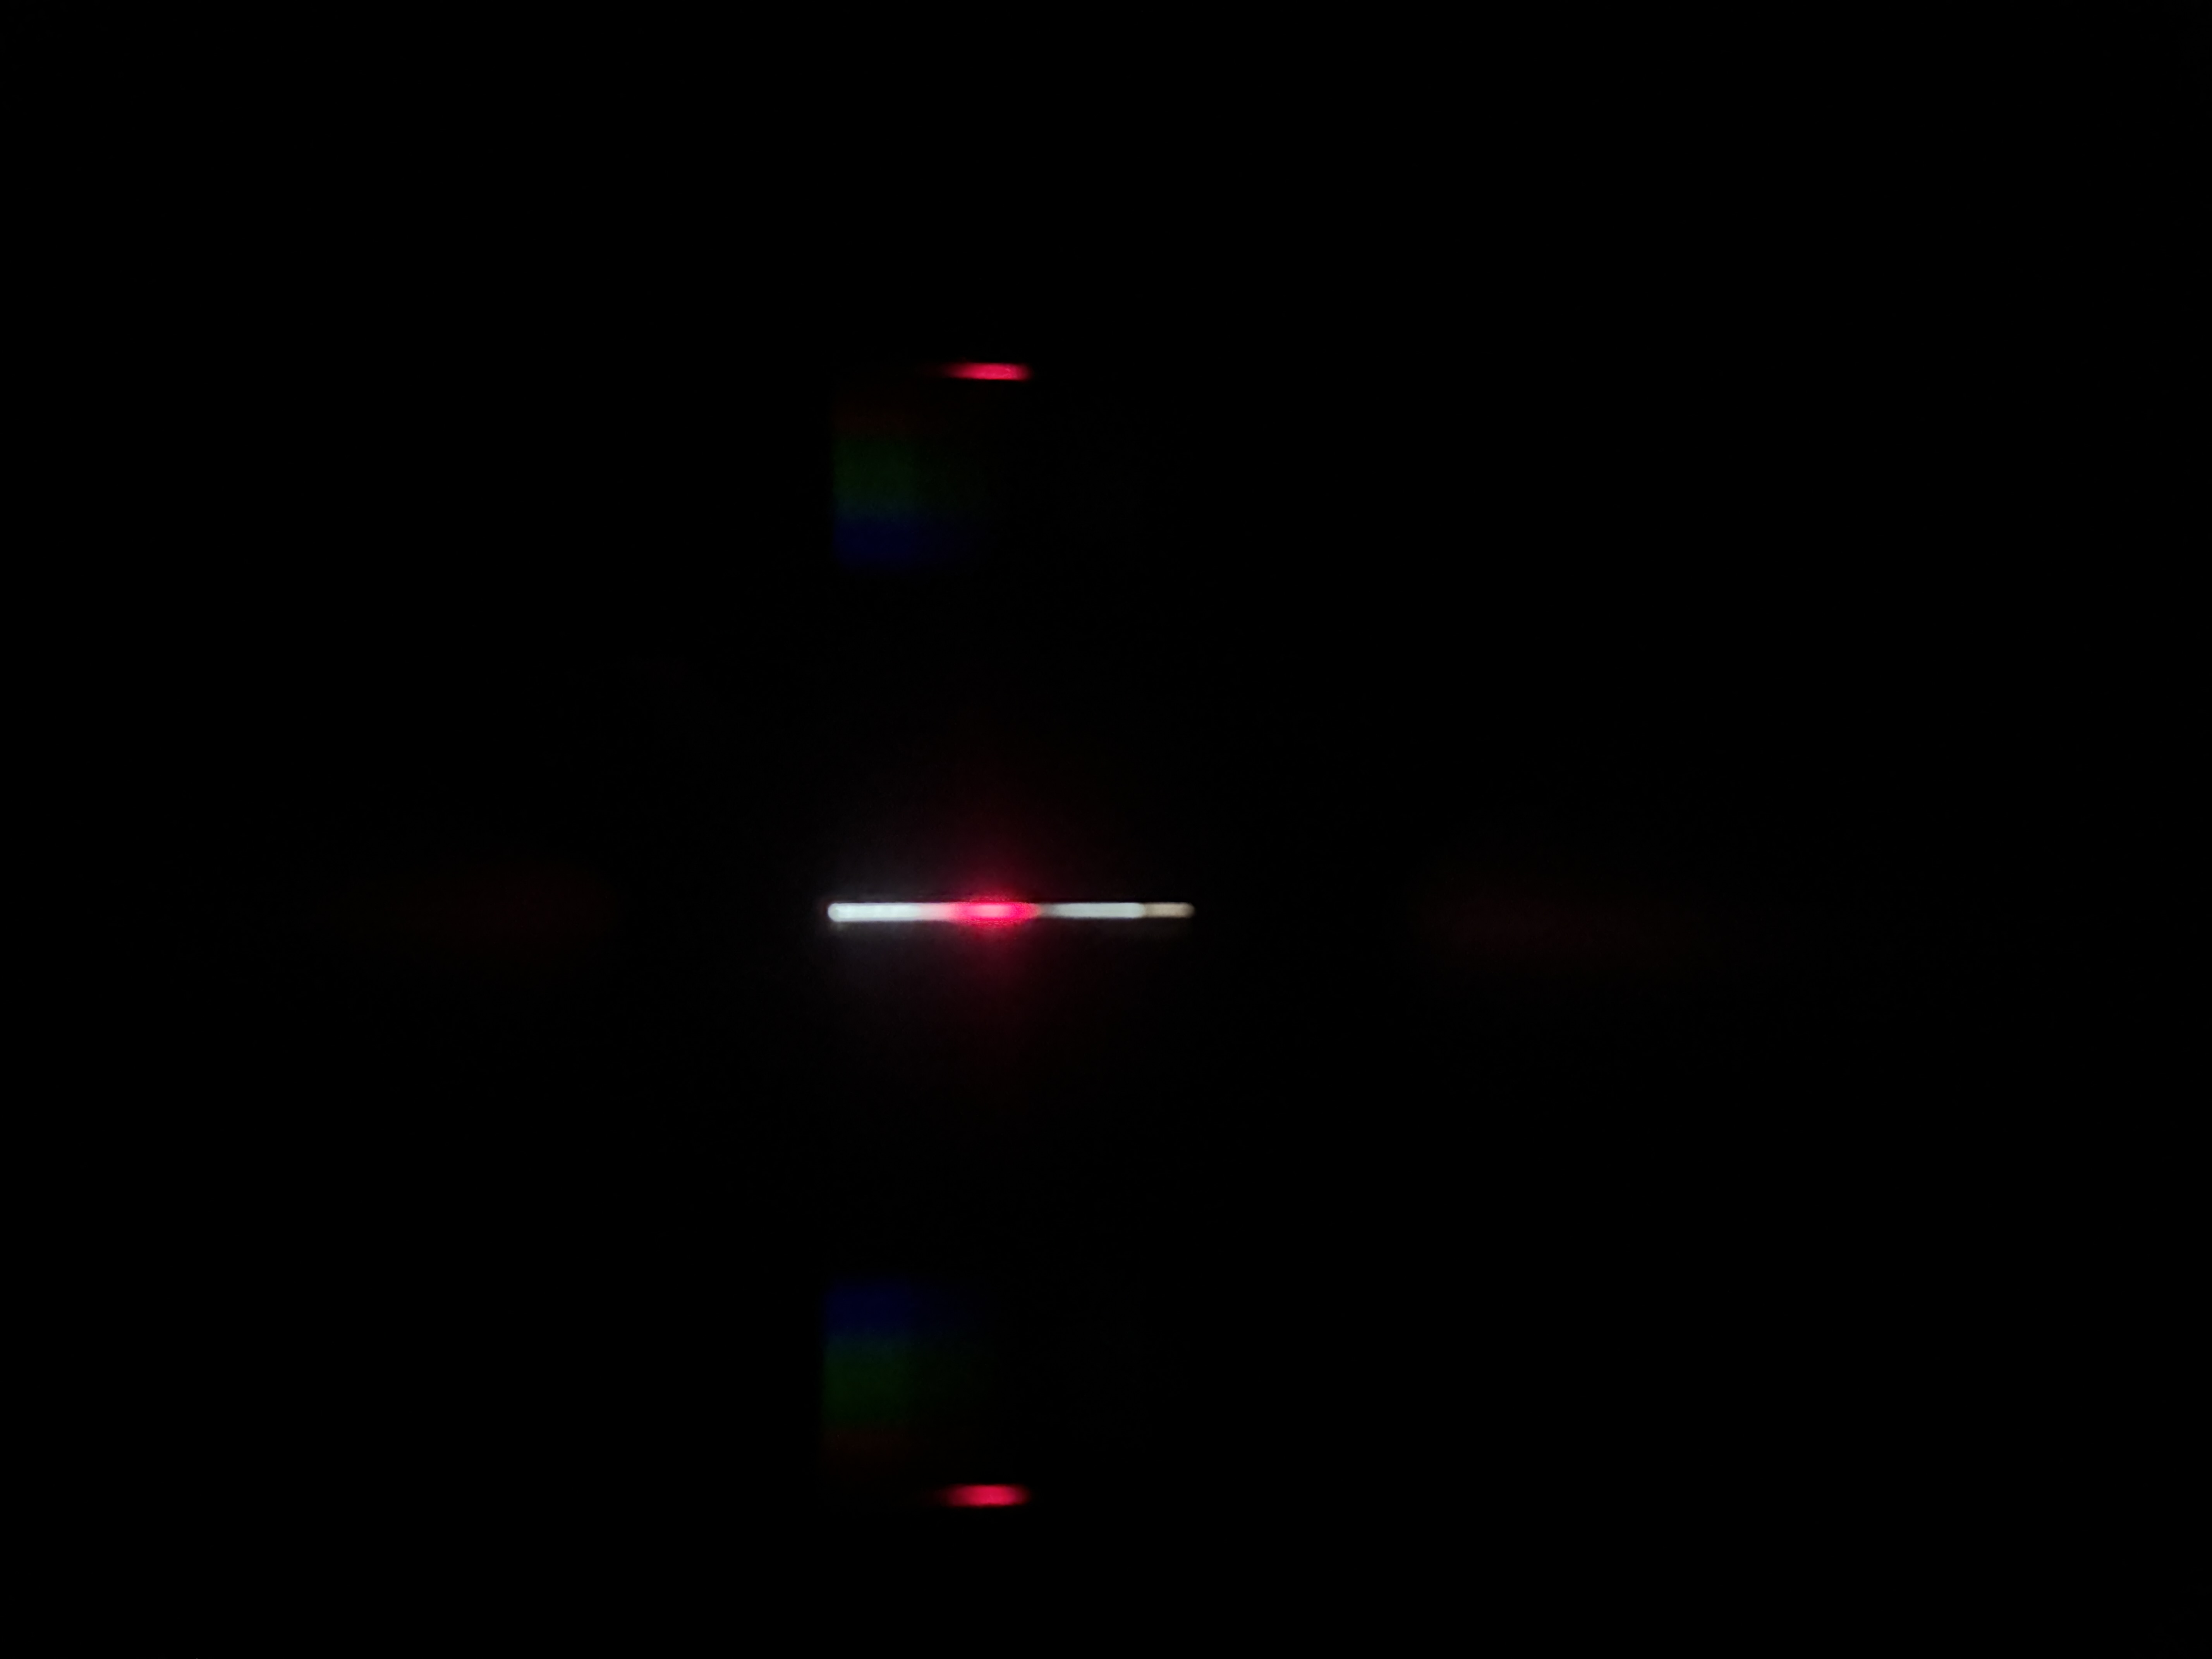
\includegraphics[width=\textwidth]{Fig_1.JPG}
                \caption{红色激光，$x=\qty{1392}{px}$}
            \end{minipage}
            \begin{minipage}{0.45\textwidth}
                \centering
                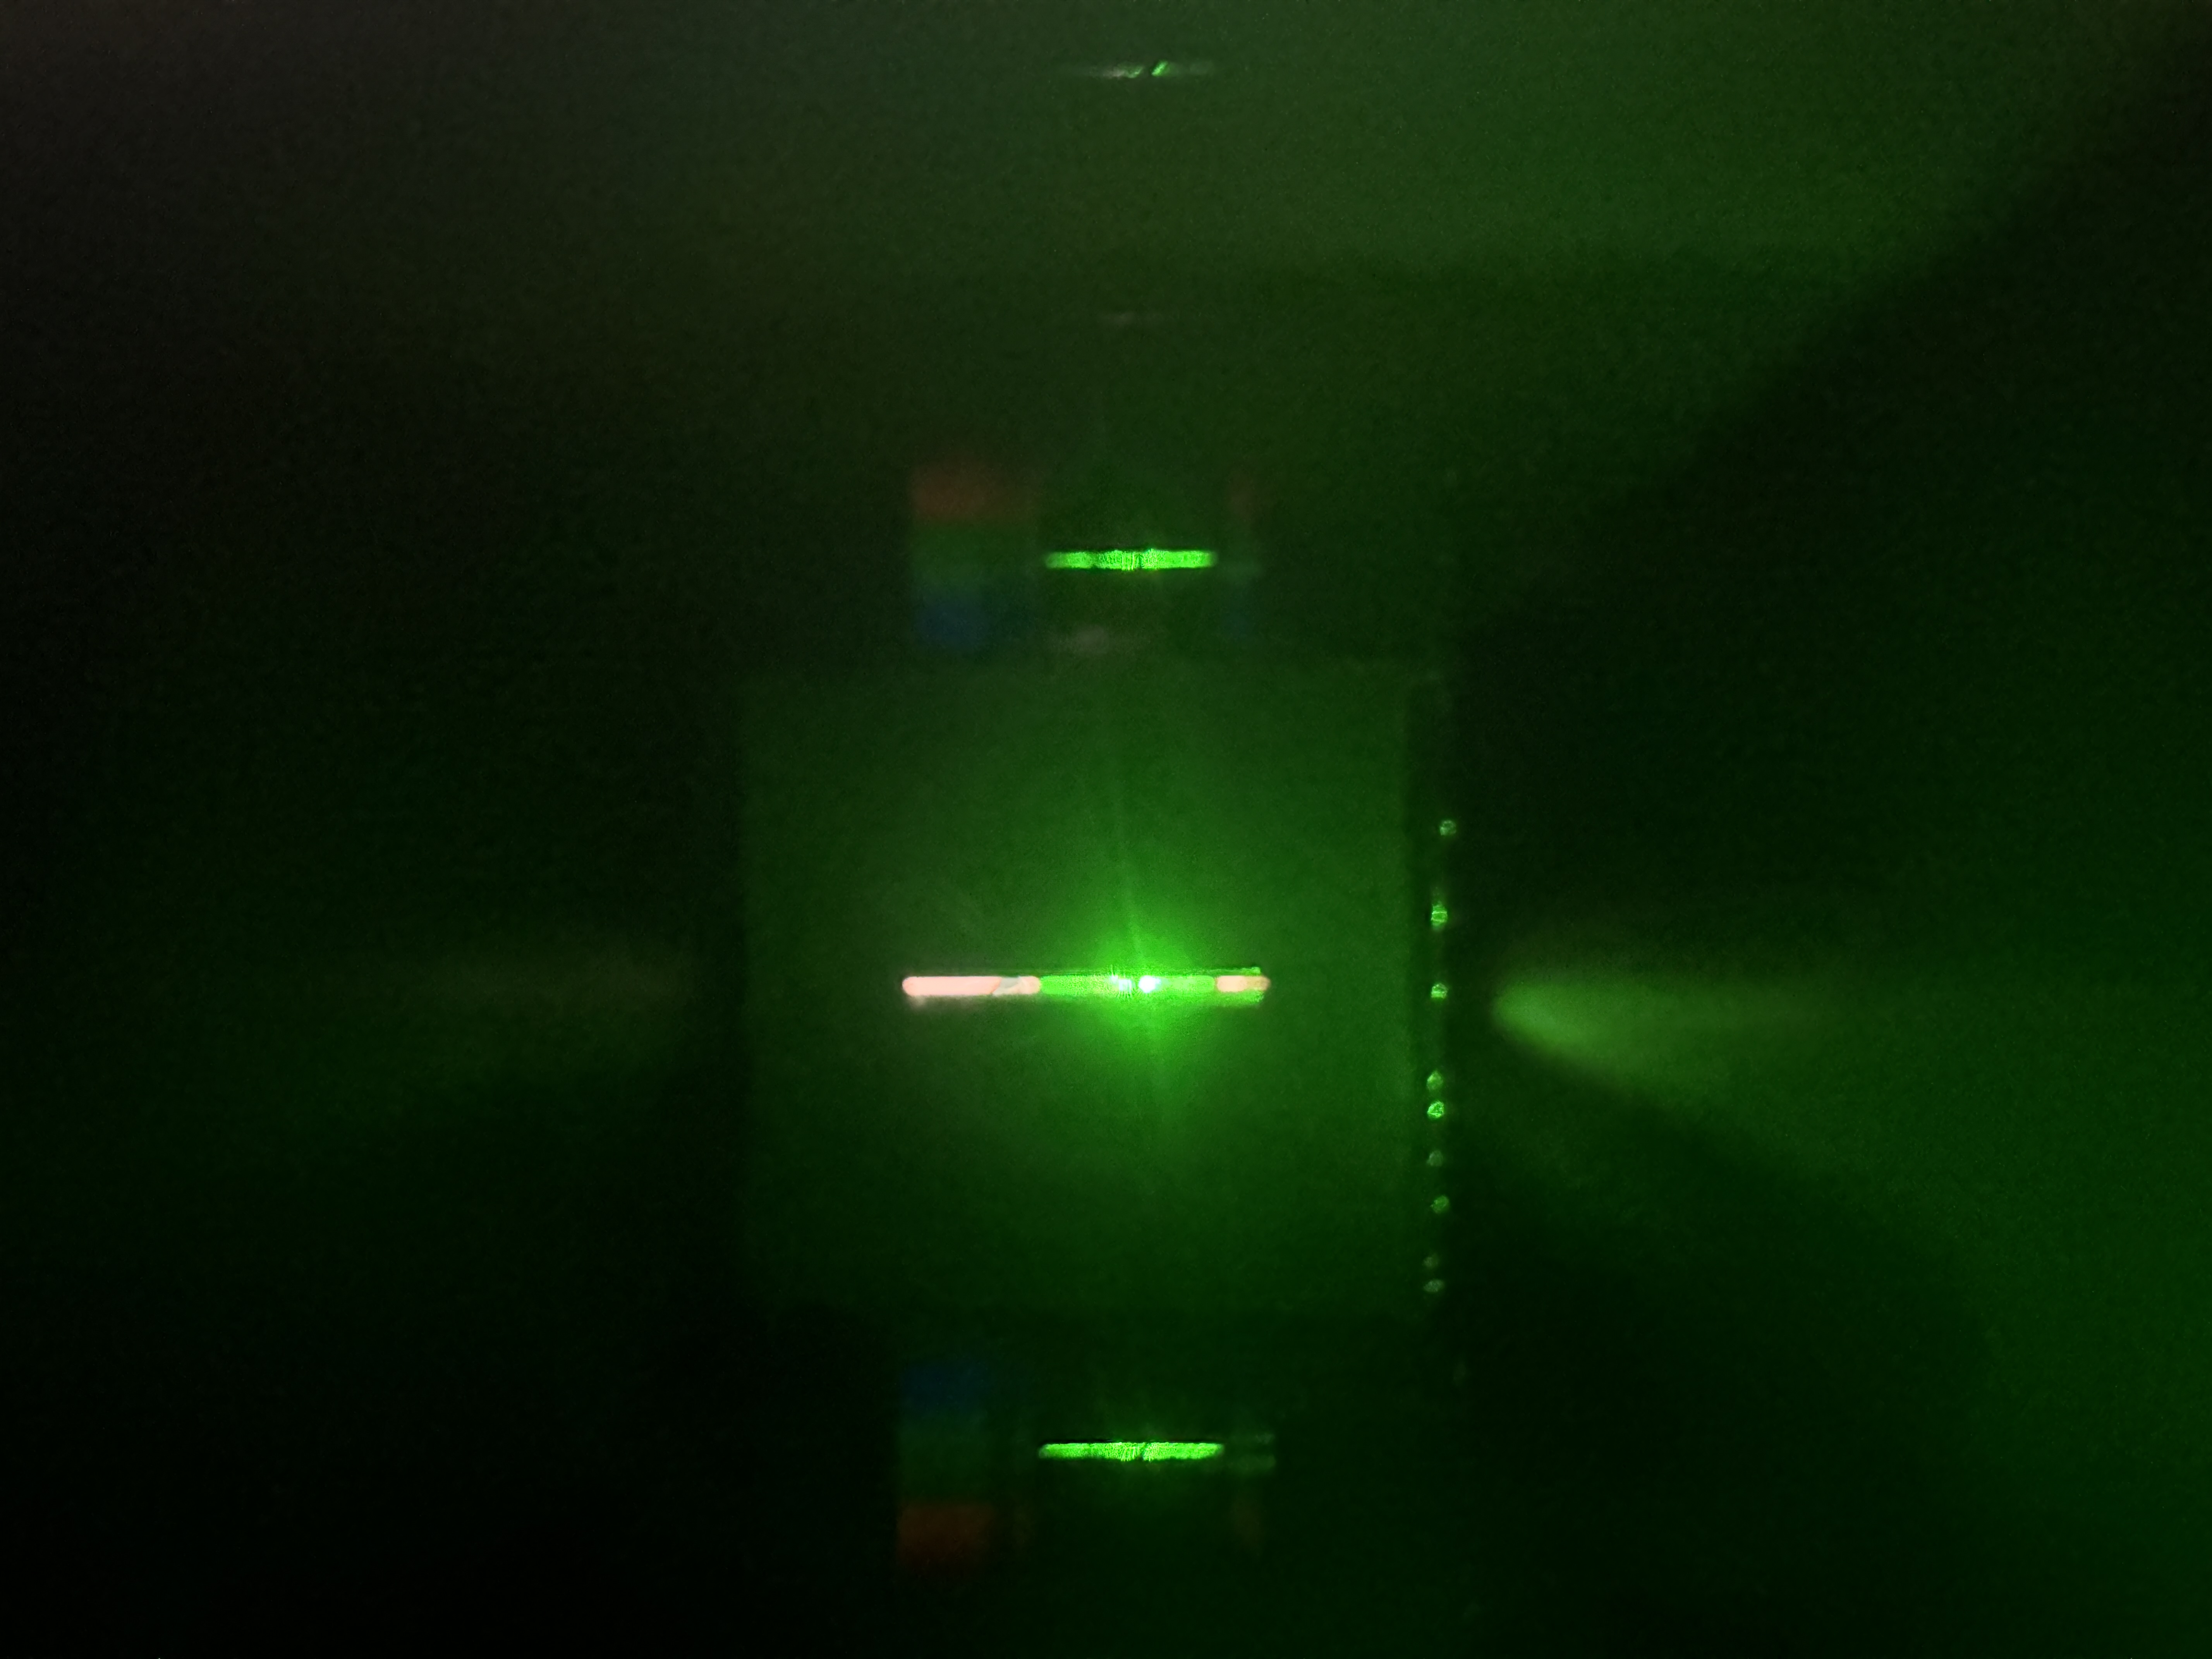
\includegraphics[width=\textwidth]{Fig_2.JPG}
                \caption{绿色激光，$x=\qty{1096}{px}$}
            \end{minipage}
            }
        \end{figure}
        利用衍射公式计算得到 $L_R =\qty{4050}{px}$，$L_G = \qty{3972}{px}$，取两者平均值，记 $L = \qty{4011}{px}$，这样得到图像中衍射图案距离与衍射光波长的关系：
        $$\lambda = d \sin\left(\arctan \frac{x}{L} \right) = \qty{2000}{\nm} \sin\left(\arctan \frac{x}{\qty{4011}{px}} \right).$$

        \item 实例分析
        \\[2.5mm]
        使用简易光谱仪记录不同光源的衍射图案，导入ImageJ后绘制灰度-距离图像，将像素距离映射为波长并截取可见光波长范围，得到如下结果：
        \begin{figure}[H]
            \centering
            \scalebox{0.85}{
            \begin{minipage}{0.45\textwidth}
                \centering
                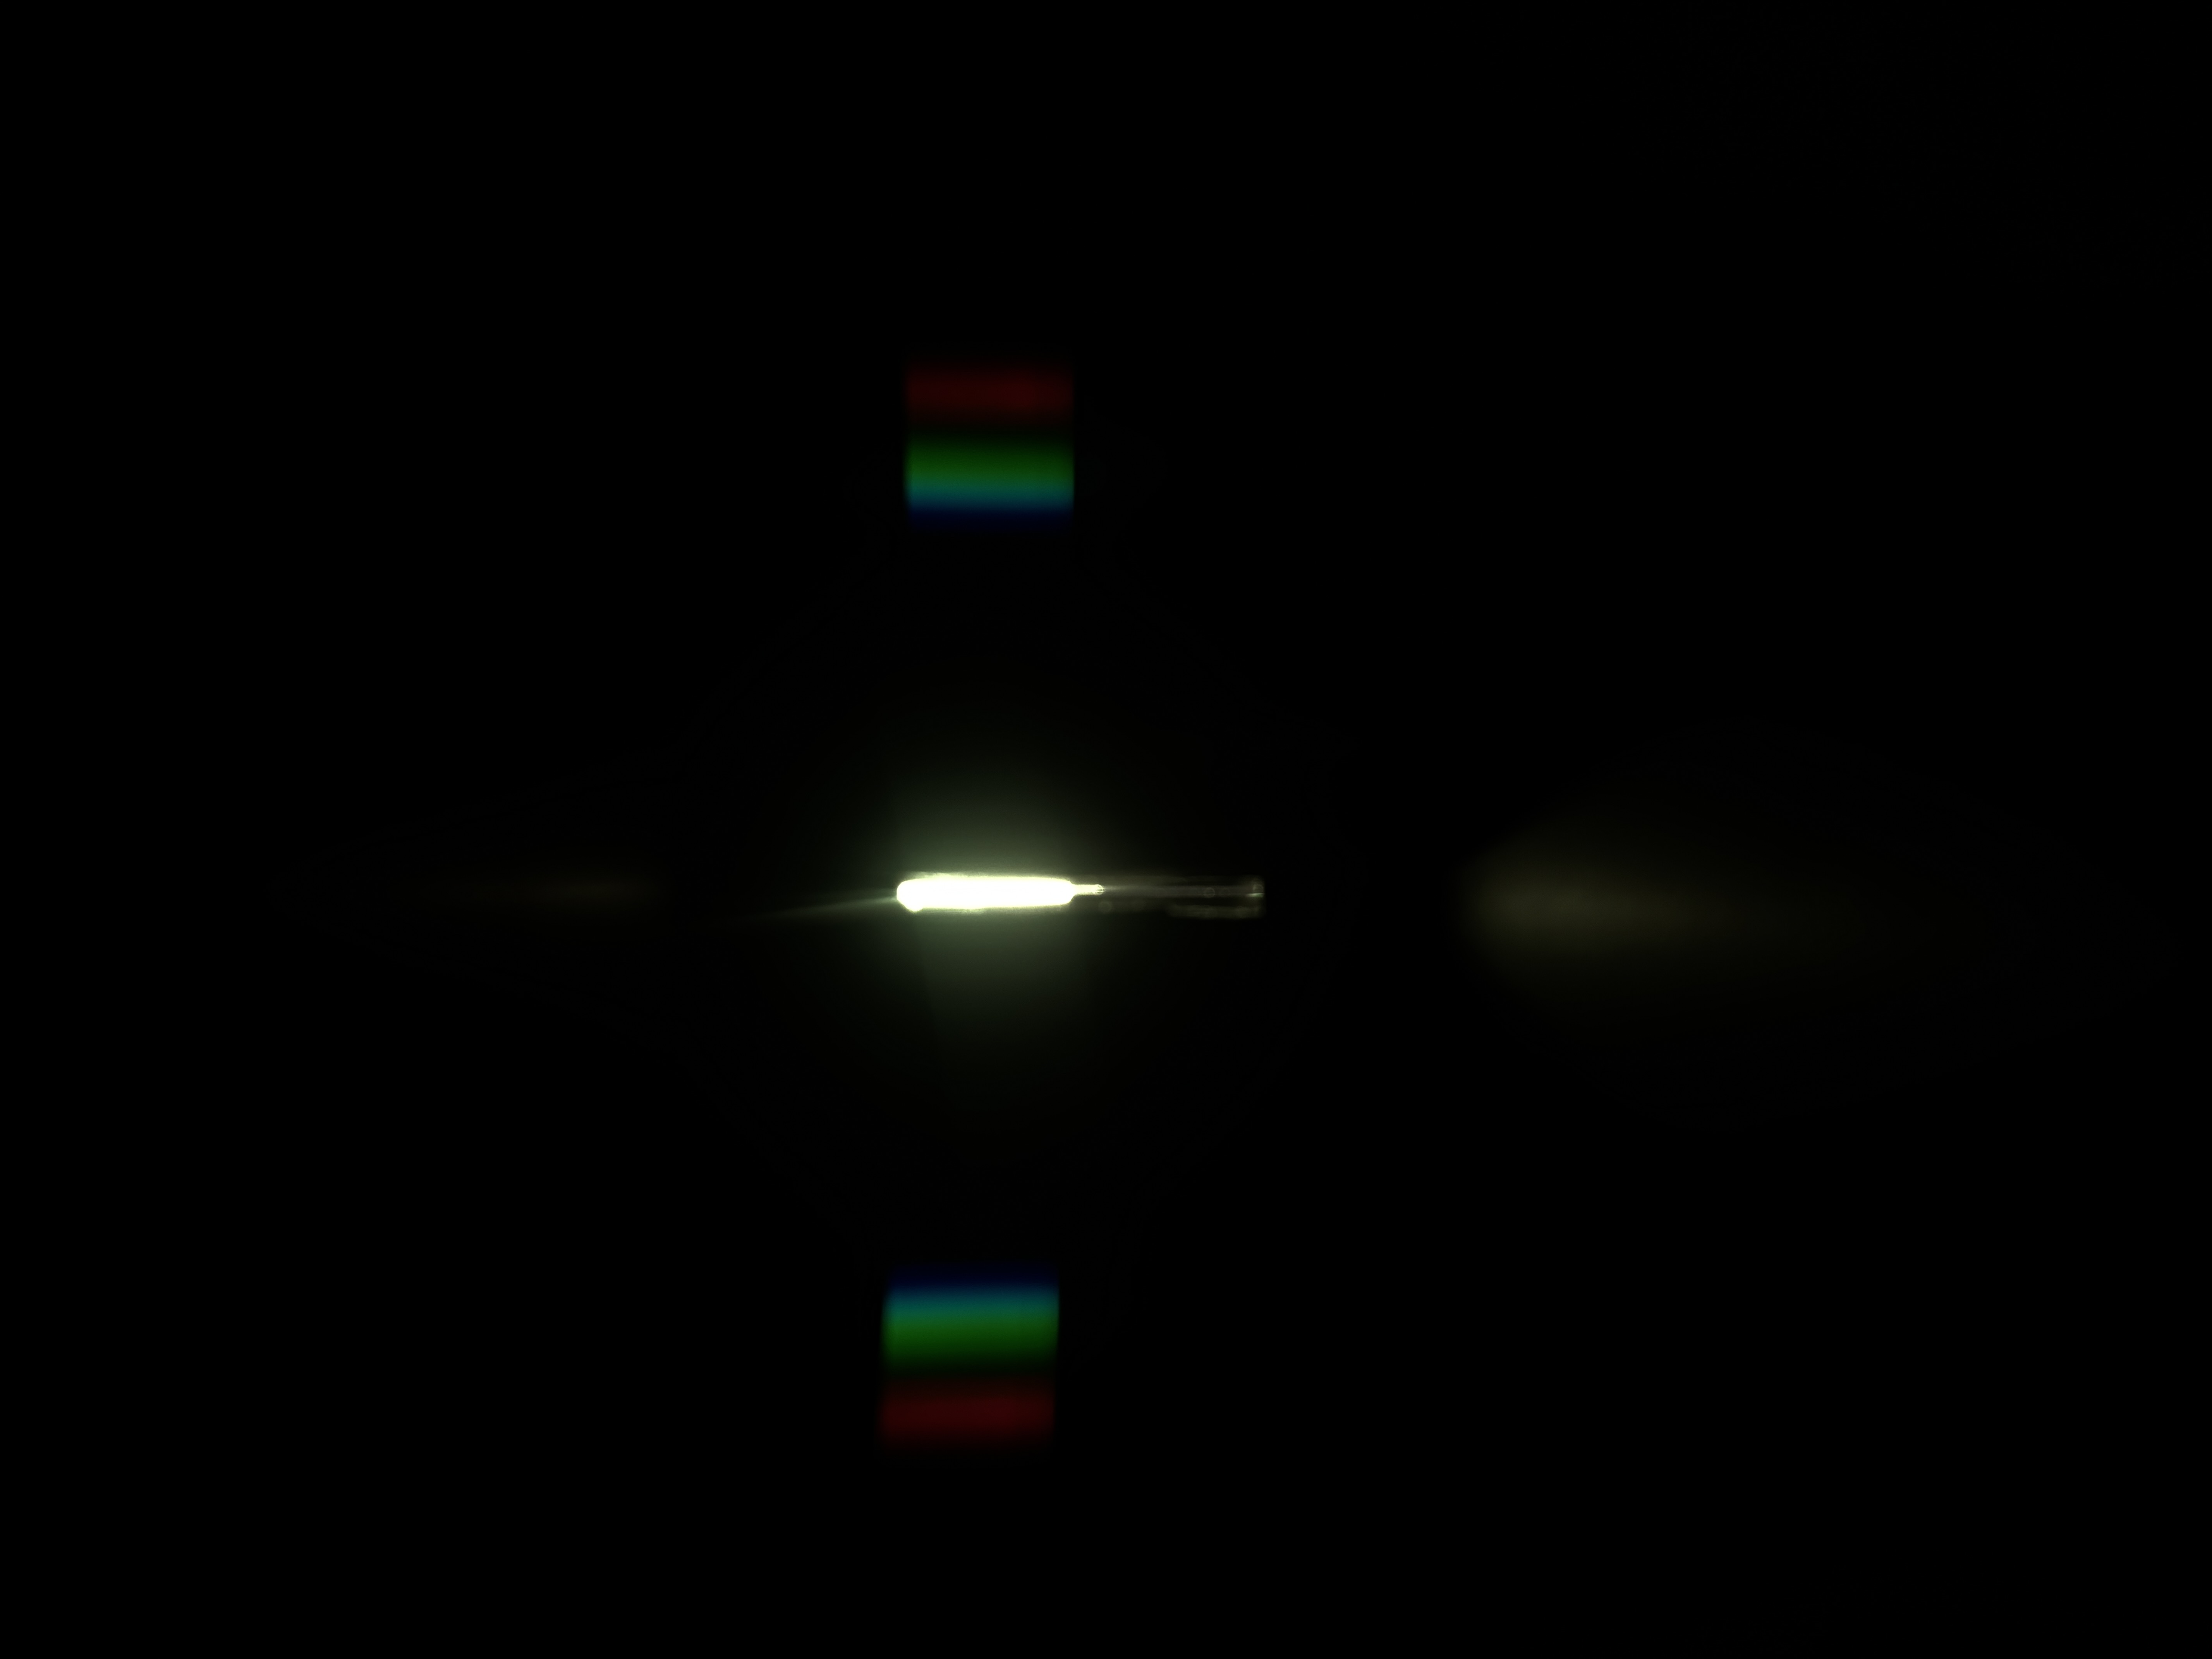
\includegraphics[width=\textwidth]{LED_1.JPG}
            \end{minipage}
            \begin{minipage}{0.45\textwidth}
                \centering
                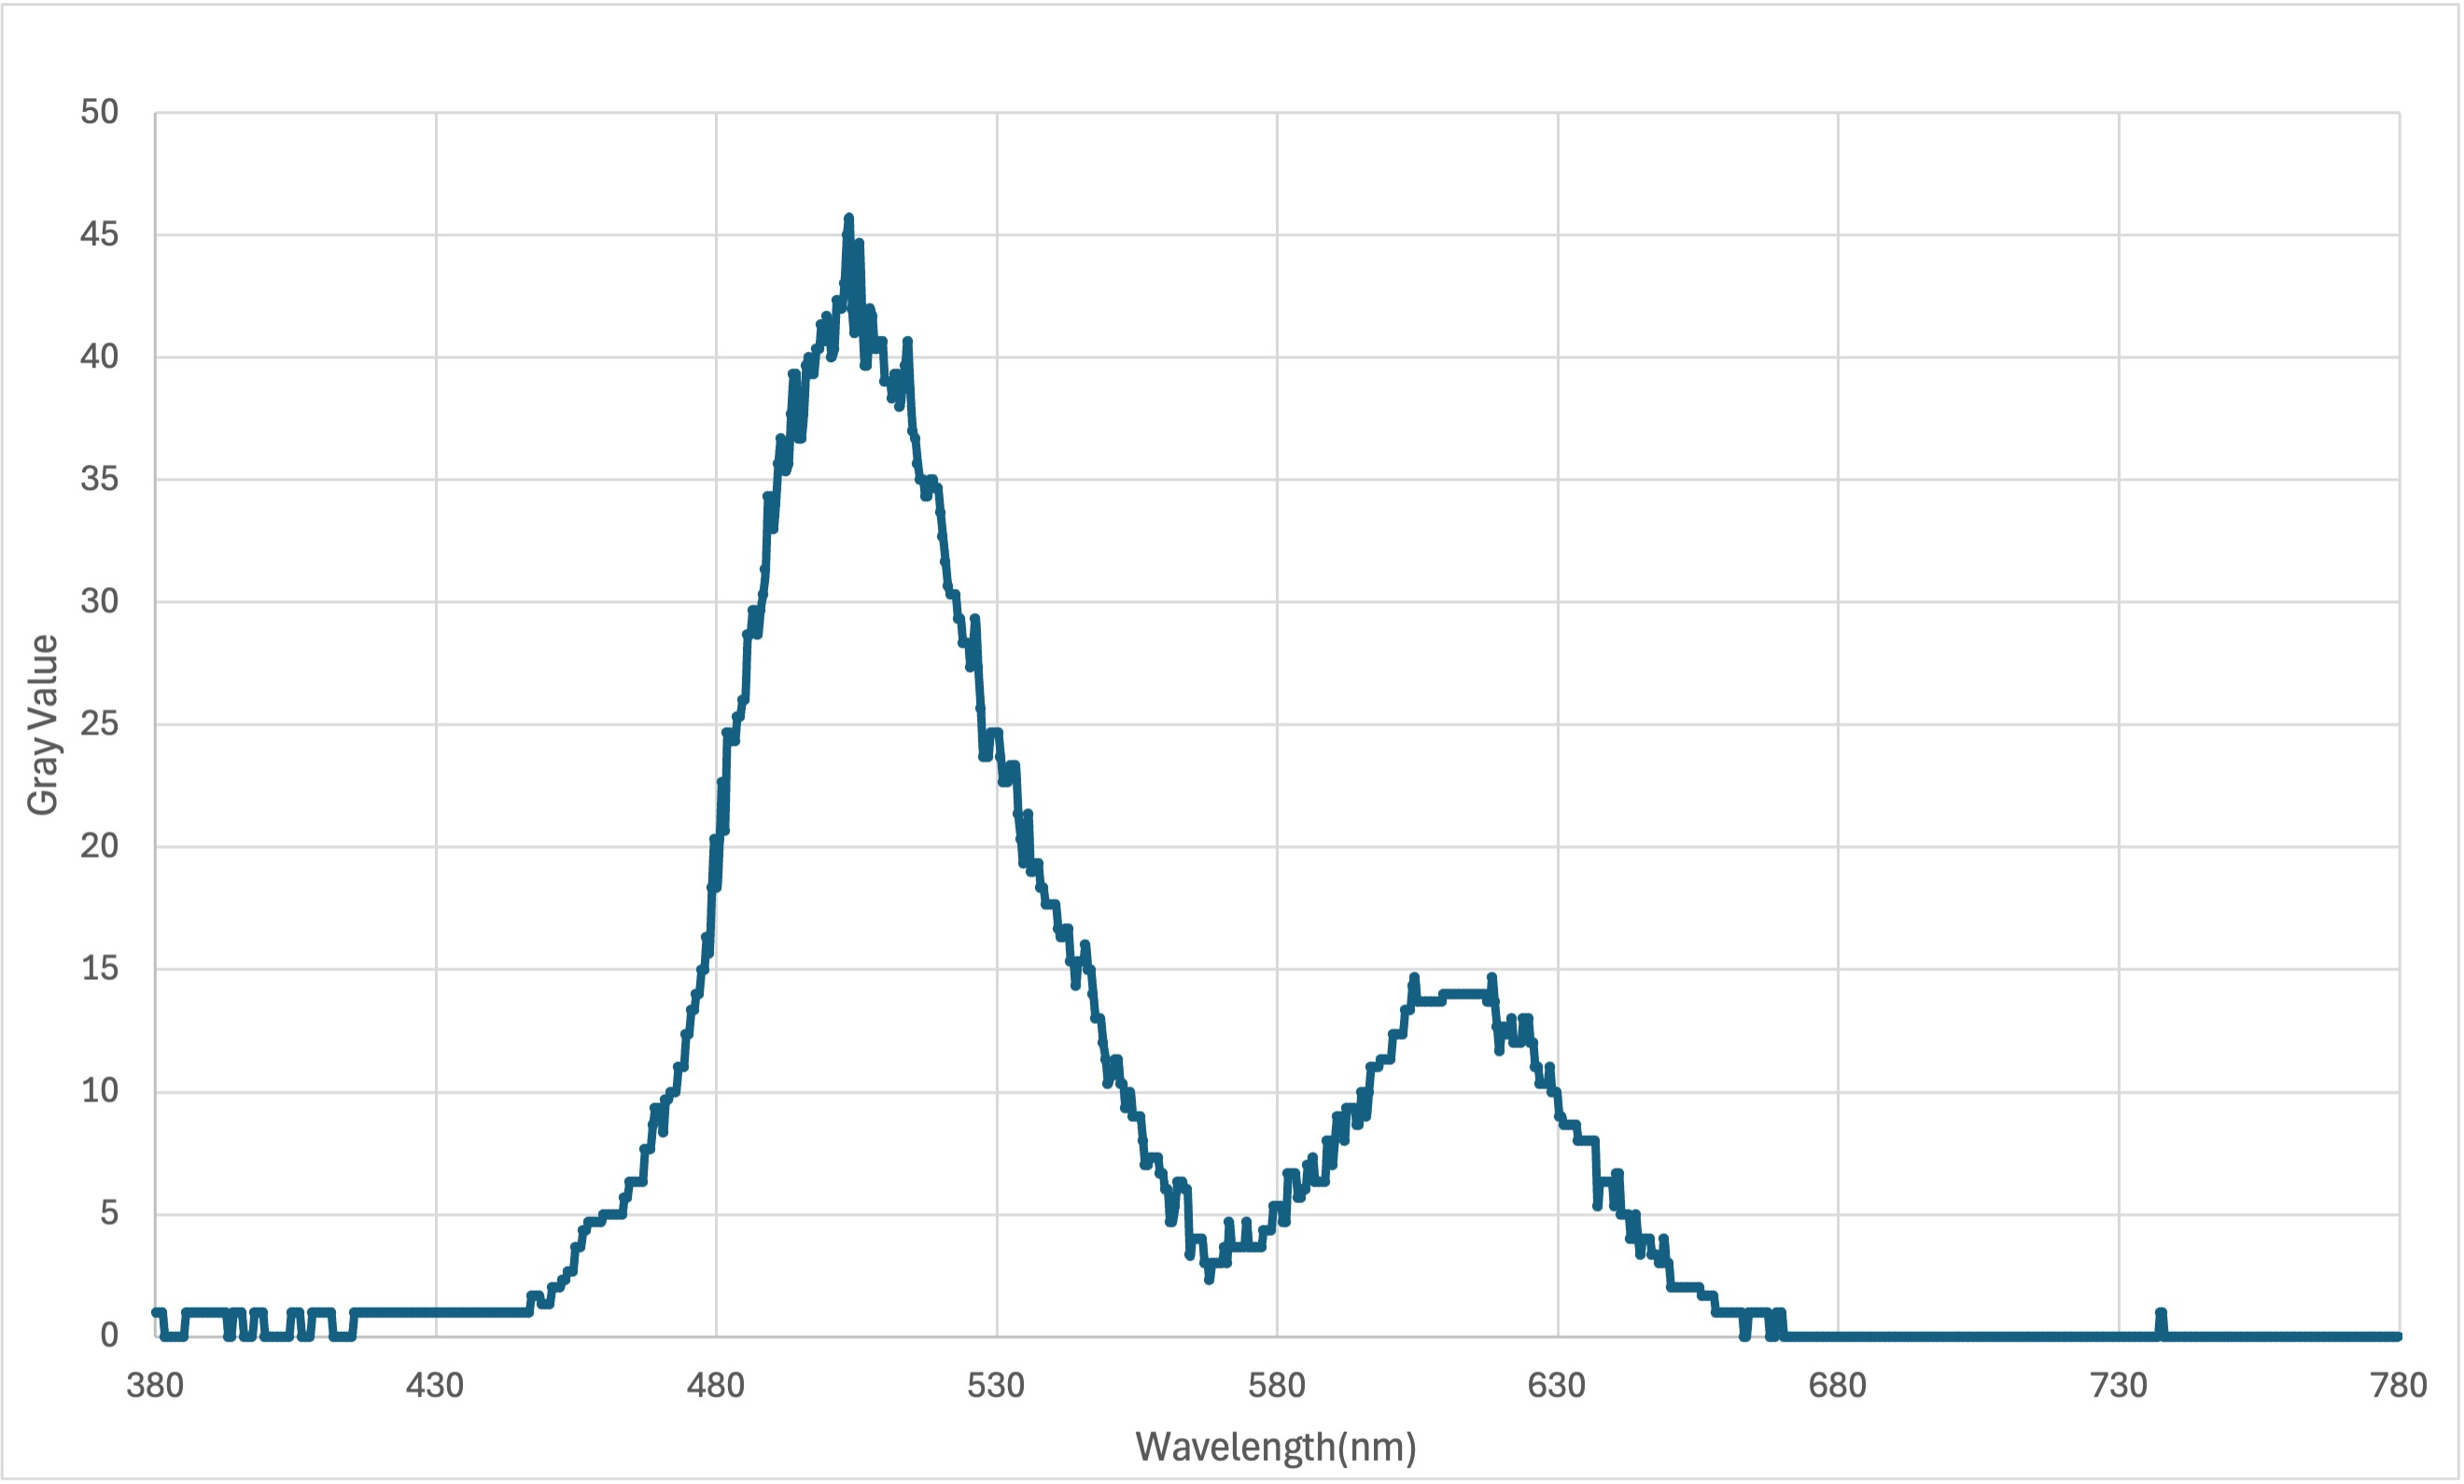
\includegraphics[width=\textwidth]{LED_1S.jpg}
            \end{minipage}}
            \caption{LED黄光}
        \end{figure}

        \begin{figure}[H]
            \centering
            \scalebox{0.85}{
            \begin{minipage}{0.45\textwidth}
                \centering
                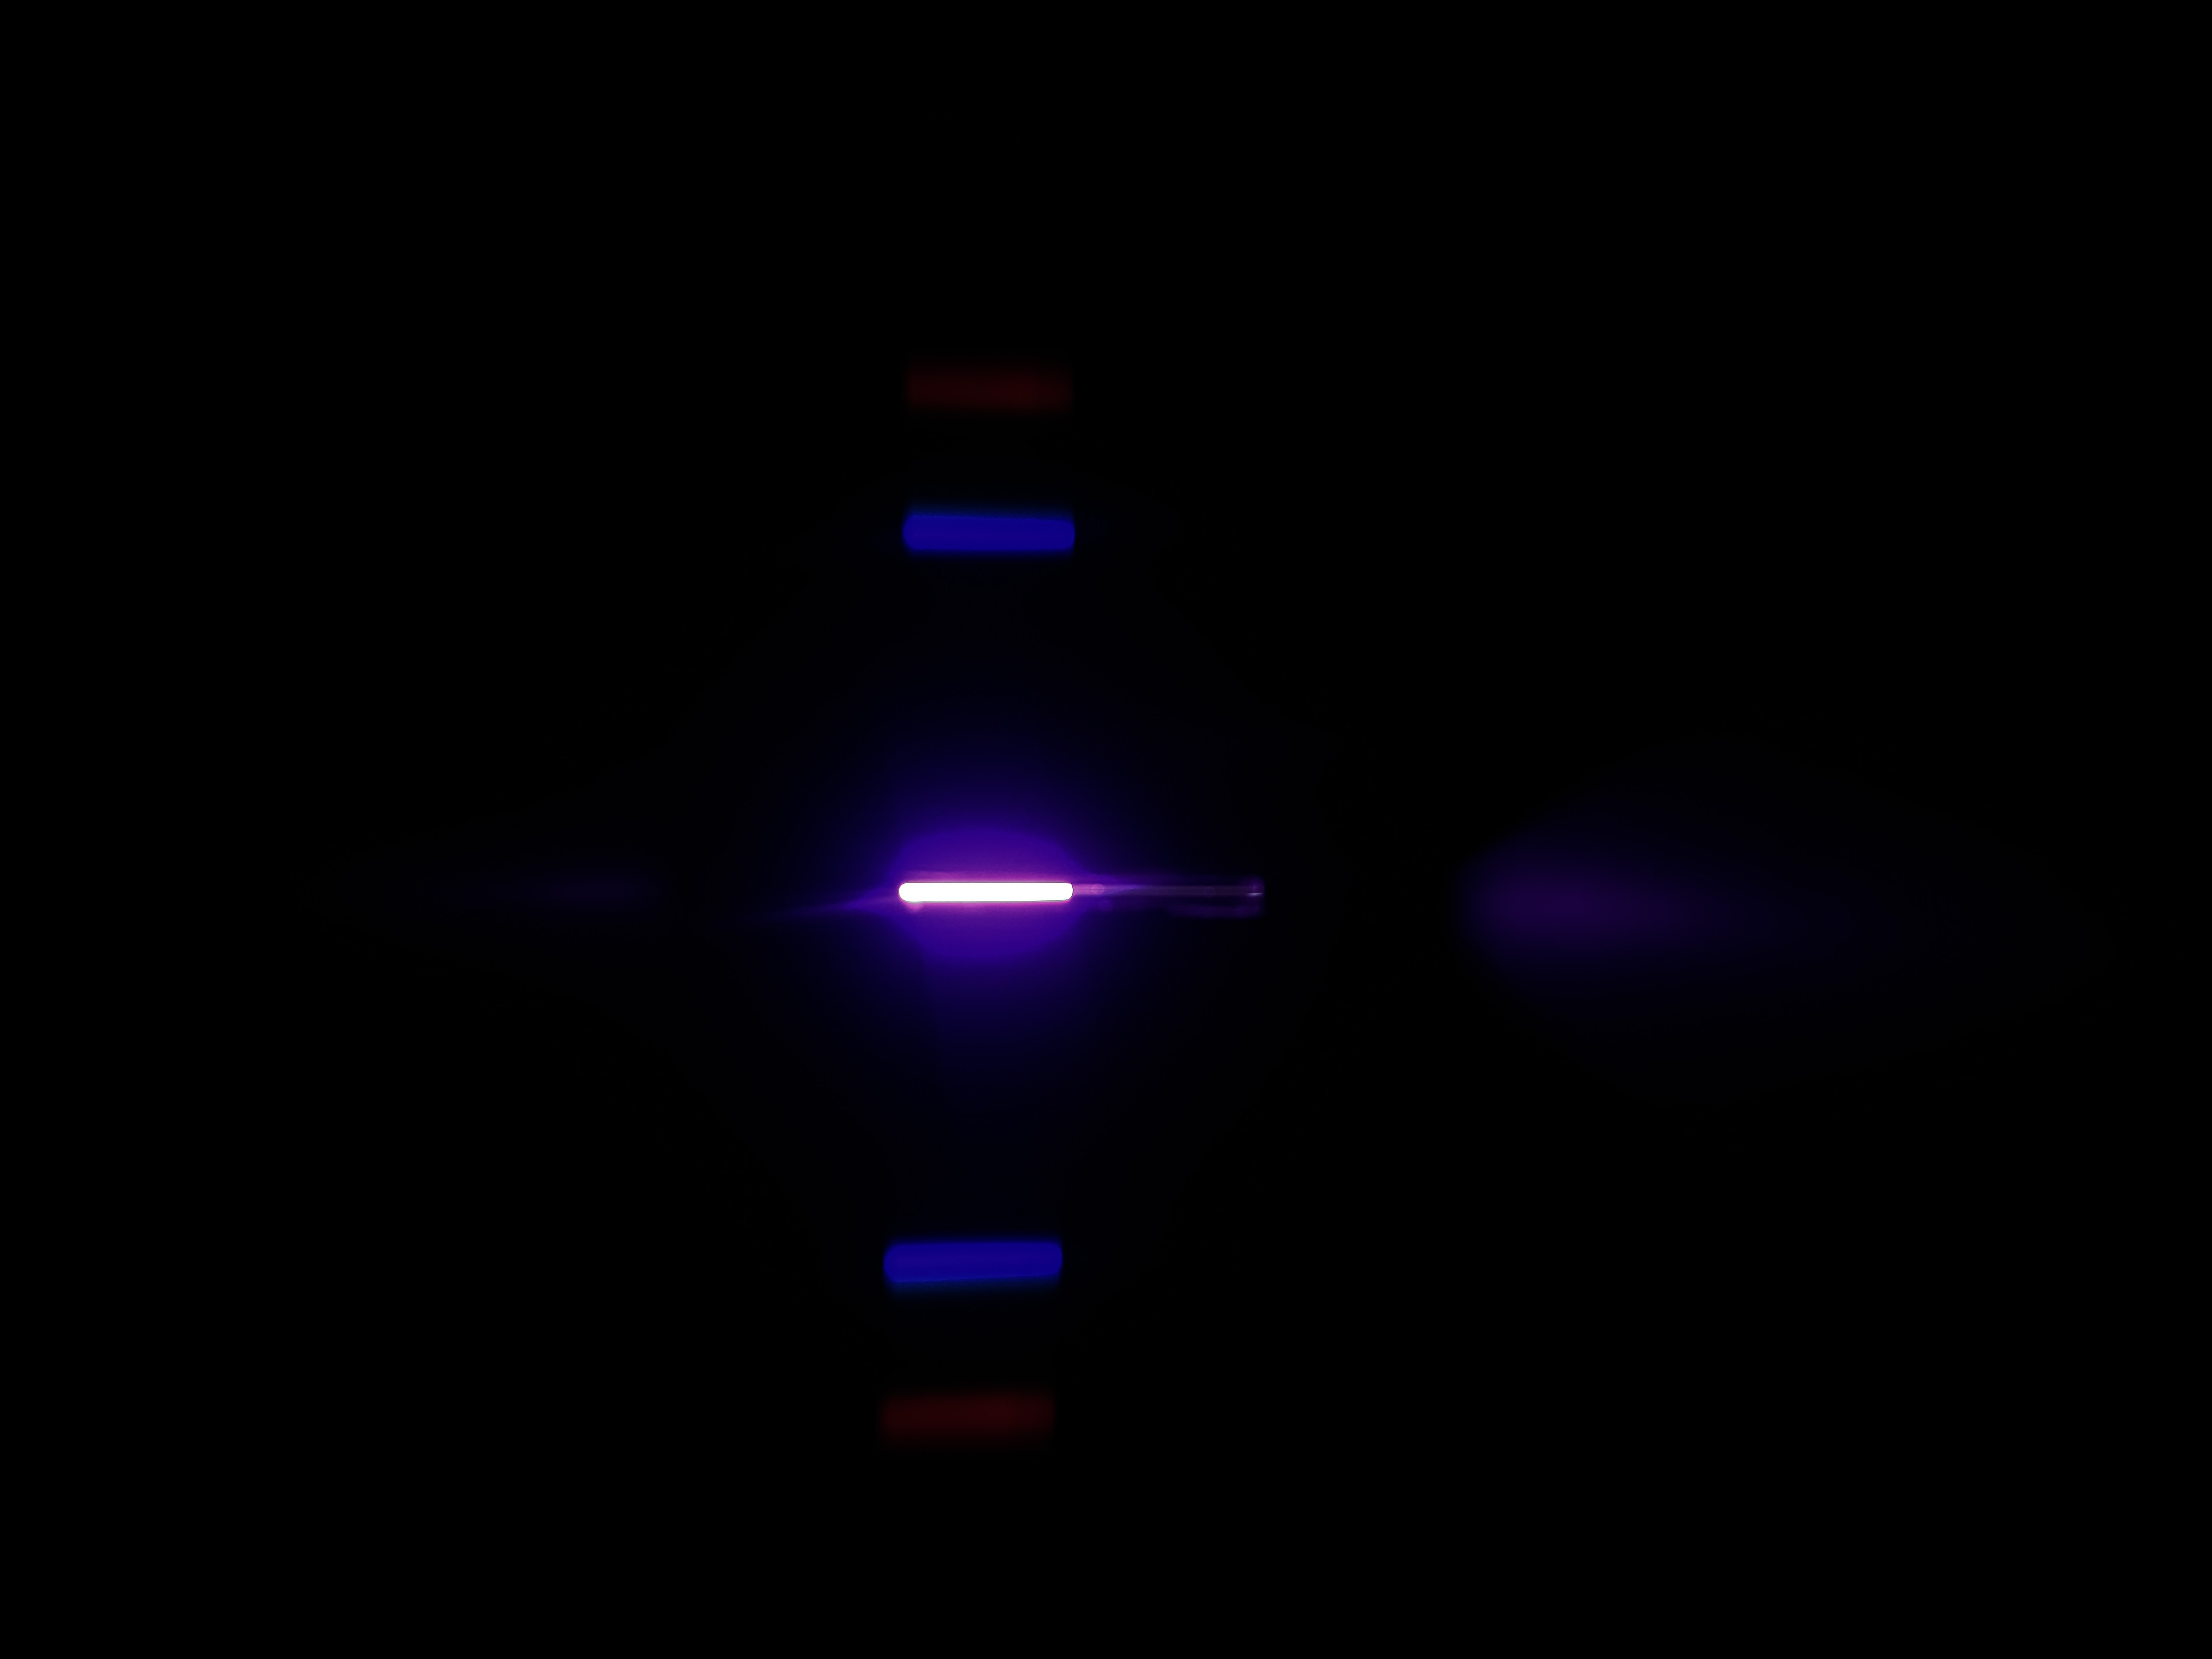
\includegraphics[width=\textwidth]{LED_2.JPG}
            \end{minipage}
            \begin{minipage}{0.45\textwidth}
                \centering
                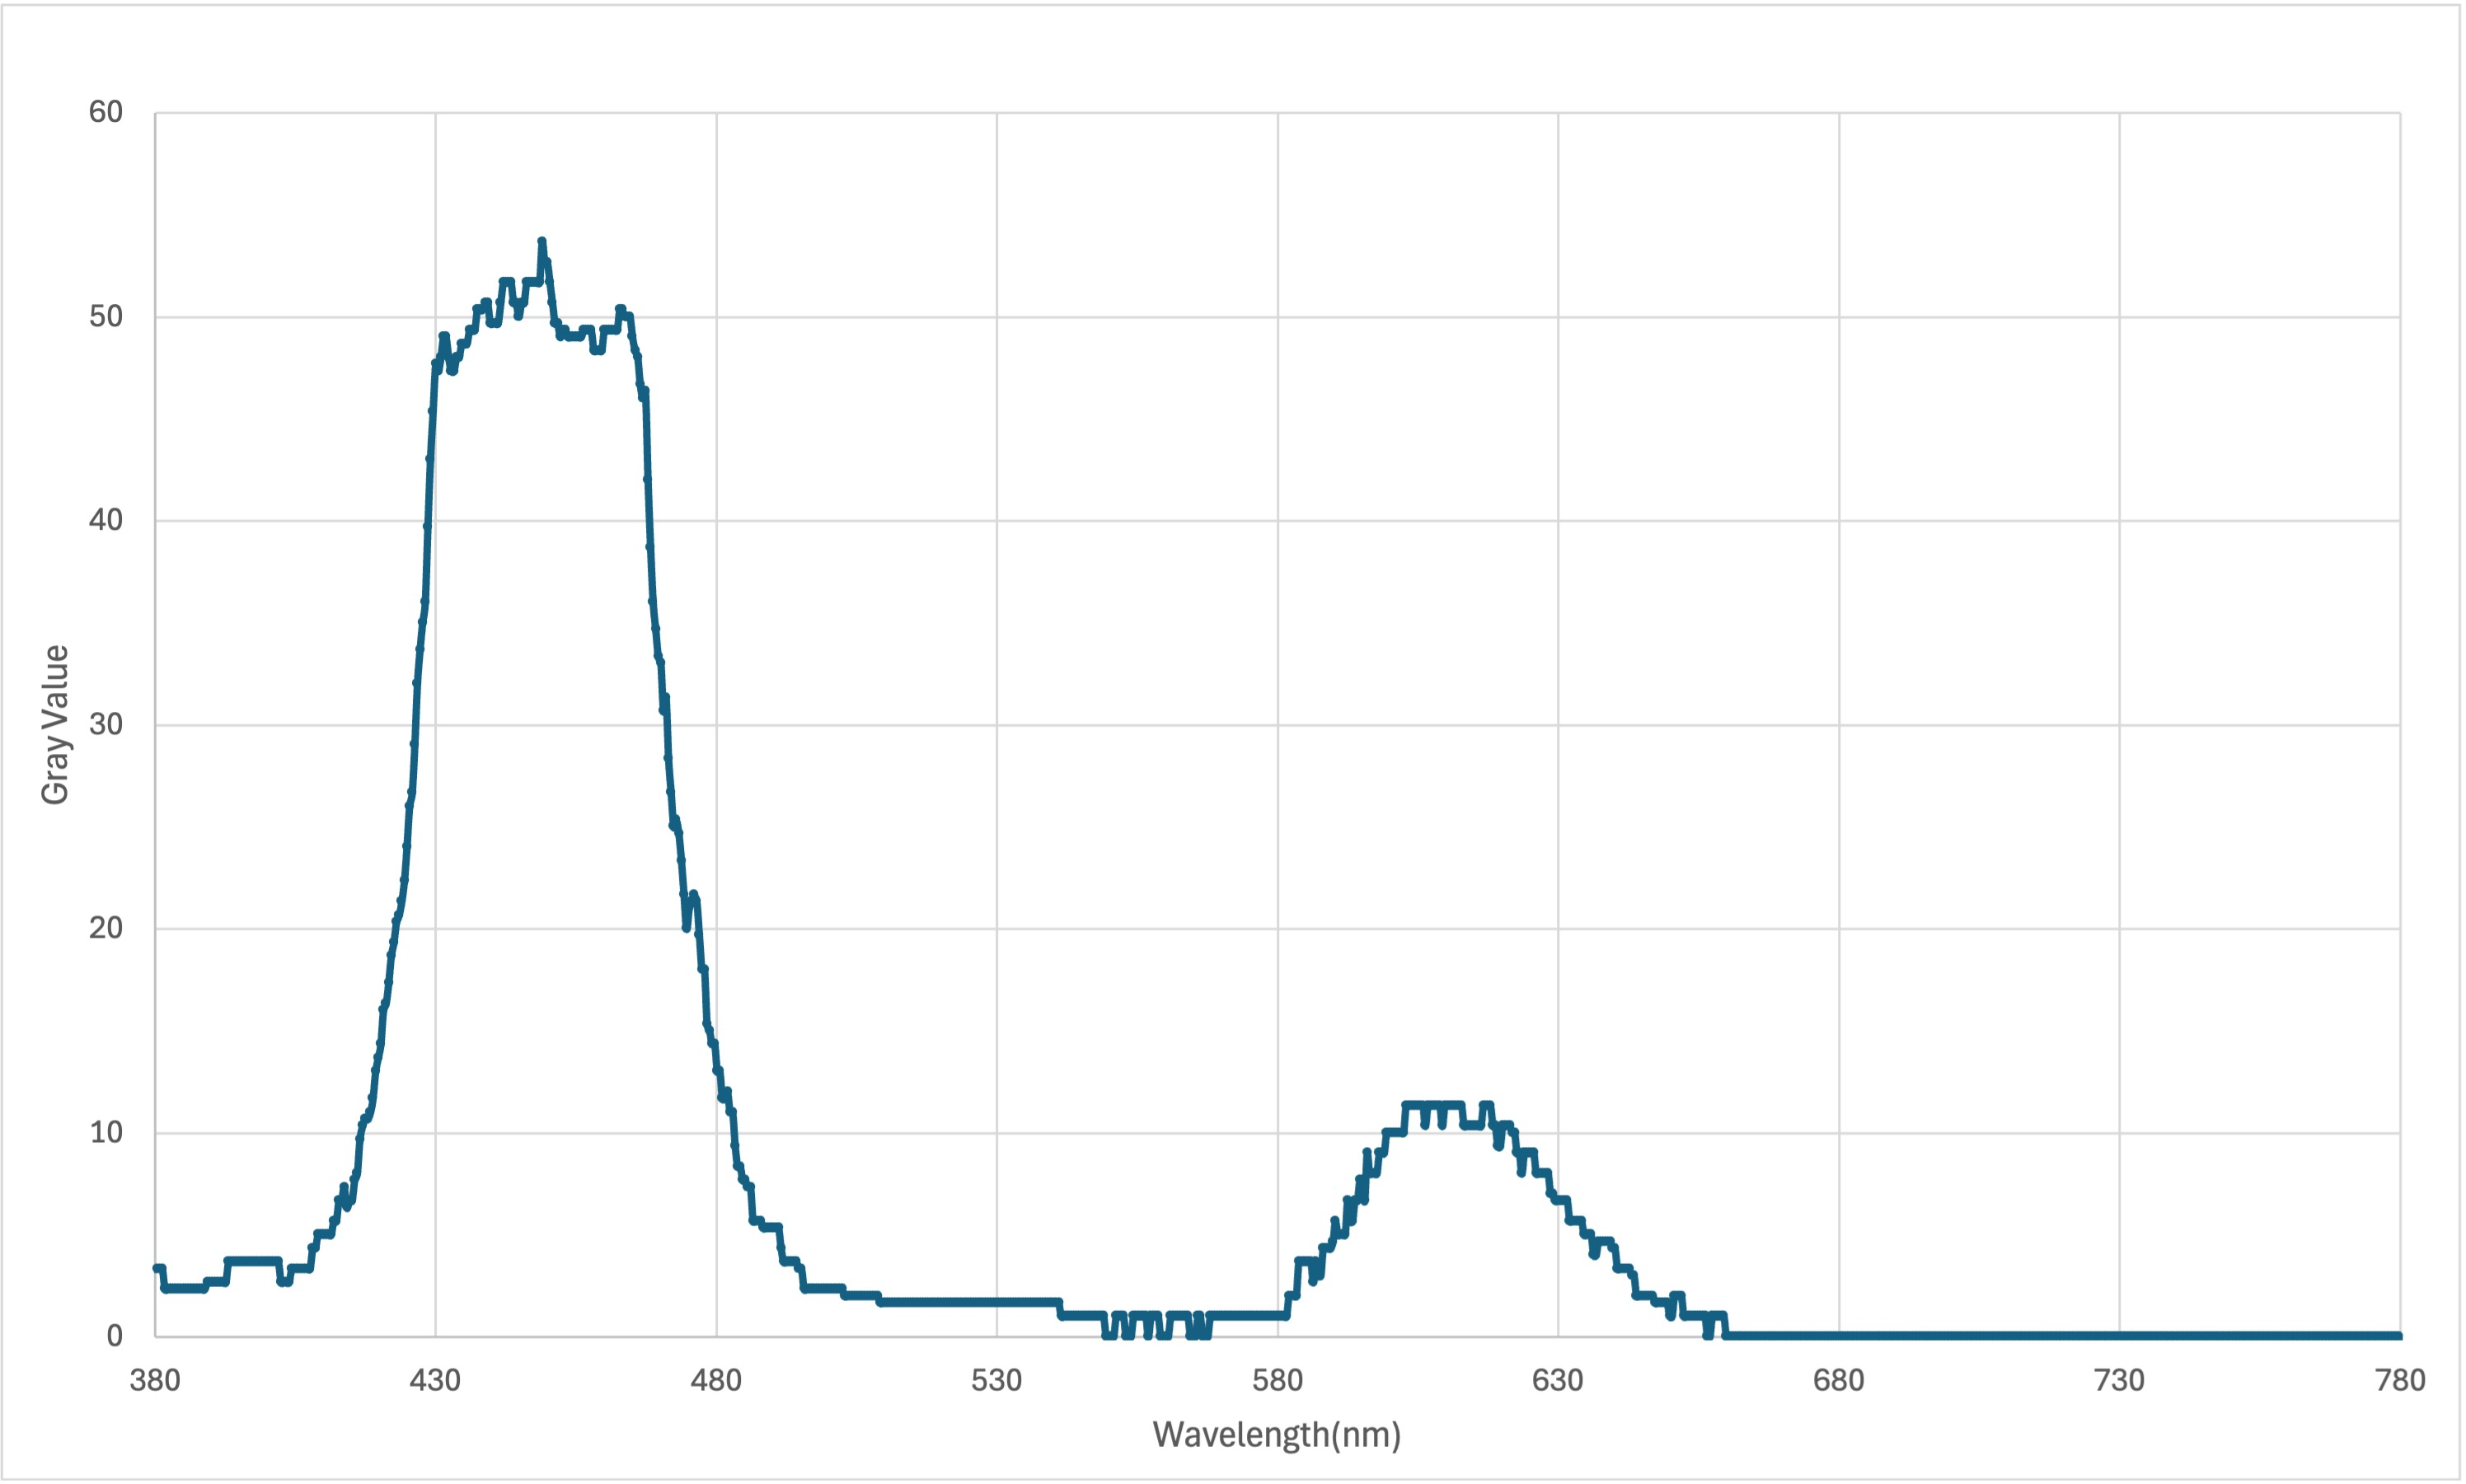
\includegraphics[width=\textwidth]{LED_2S.jpg}
            \end{minipage}
            }
            \caption{LED紫光}
        \end{figure}
        
        \begin{figure}[H]
            \centering
            \scalebox{0.85}{
            \begin{minipage}{0.45\textwidth}
                \centering
                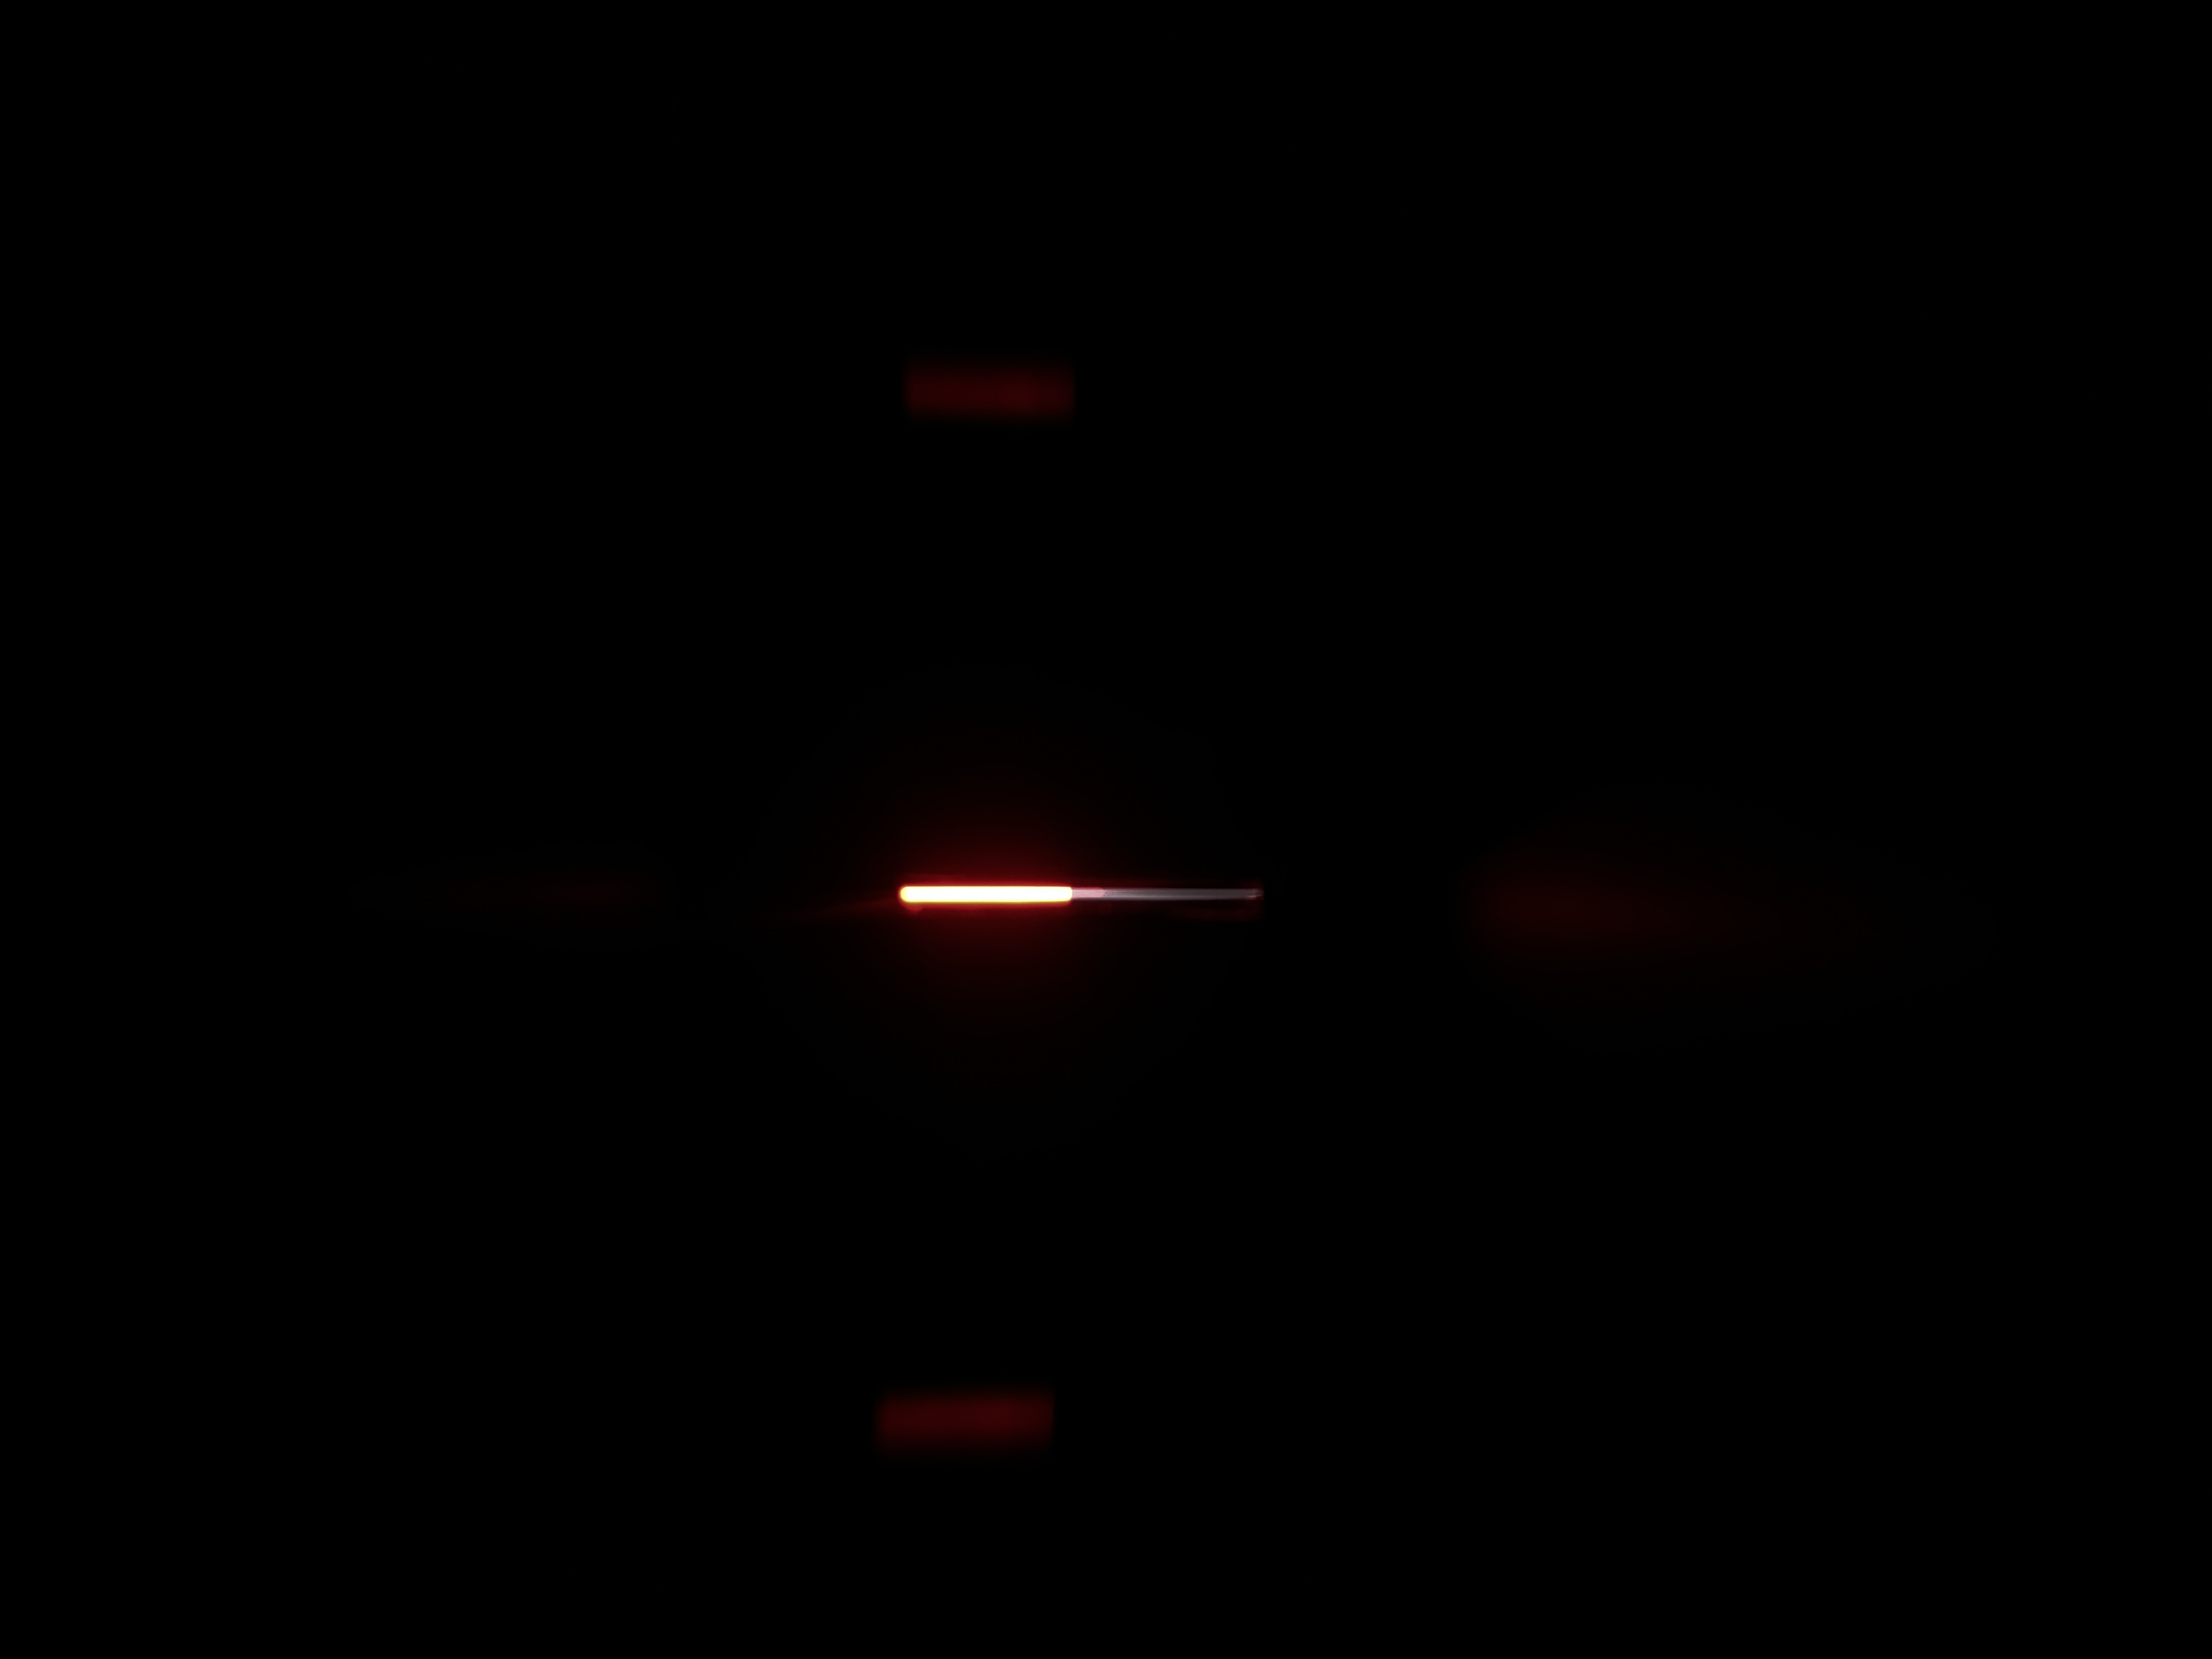
\includegraphics[width=\textwidth]{LED_3.JPG}
            \end{minipage}
            \begin{minipage}{0.45\textwidth}
                \centering
                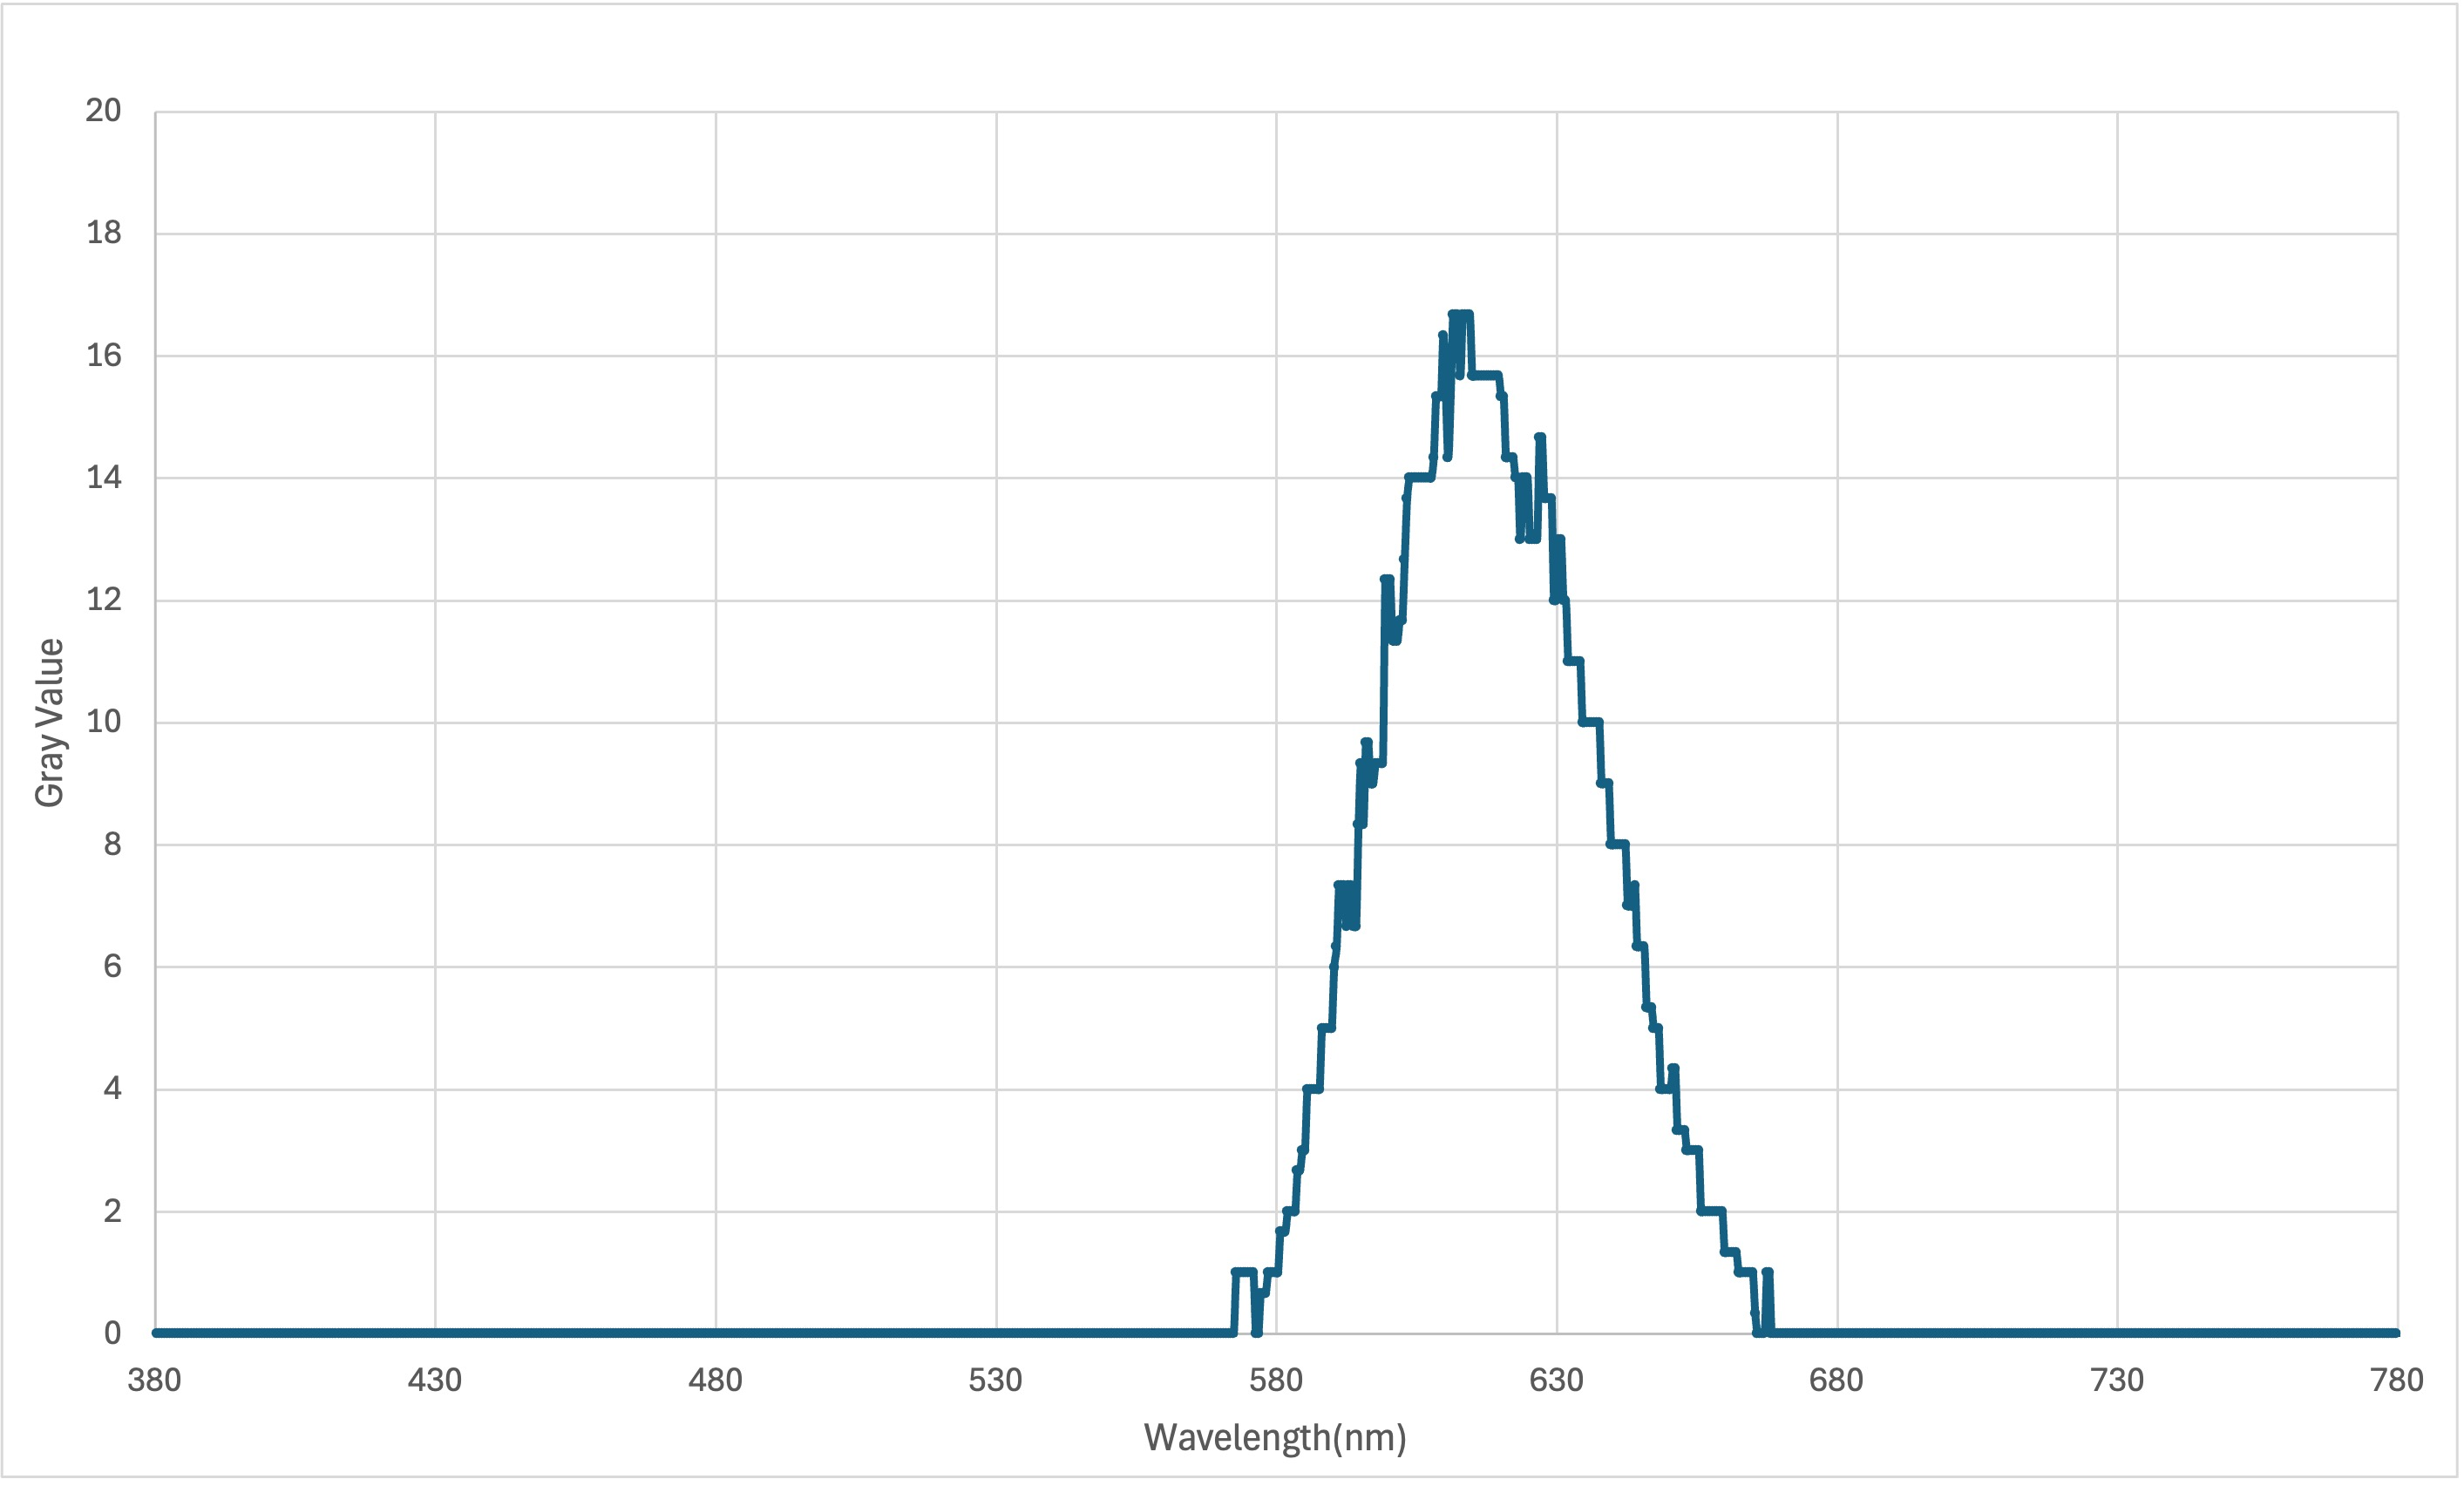
\includegraphics[width=\textwidth]{LED_3S.jpg}
            \end{minipage}
            }
            \caption{LED红光}
        \end{figure}
        
        \begin{figure}[H]
            \centering
            \scalebox{0.85}{
            \begin{minipage}{0.45\textwidth}
                \centering
                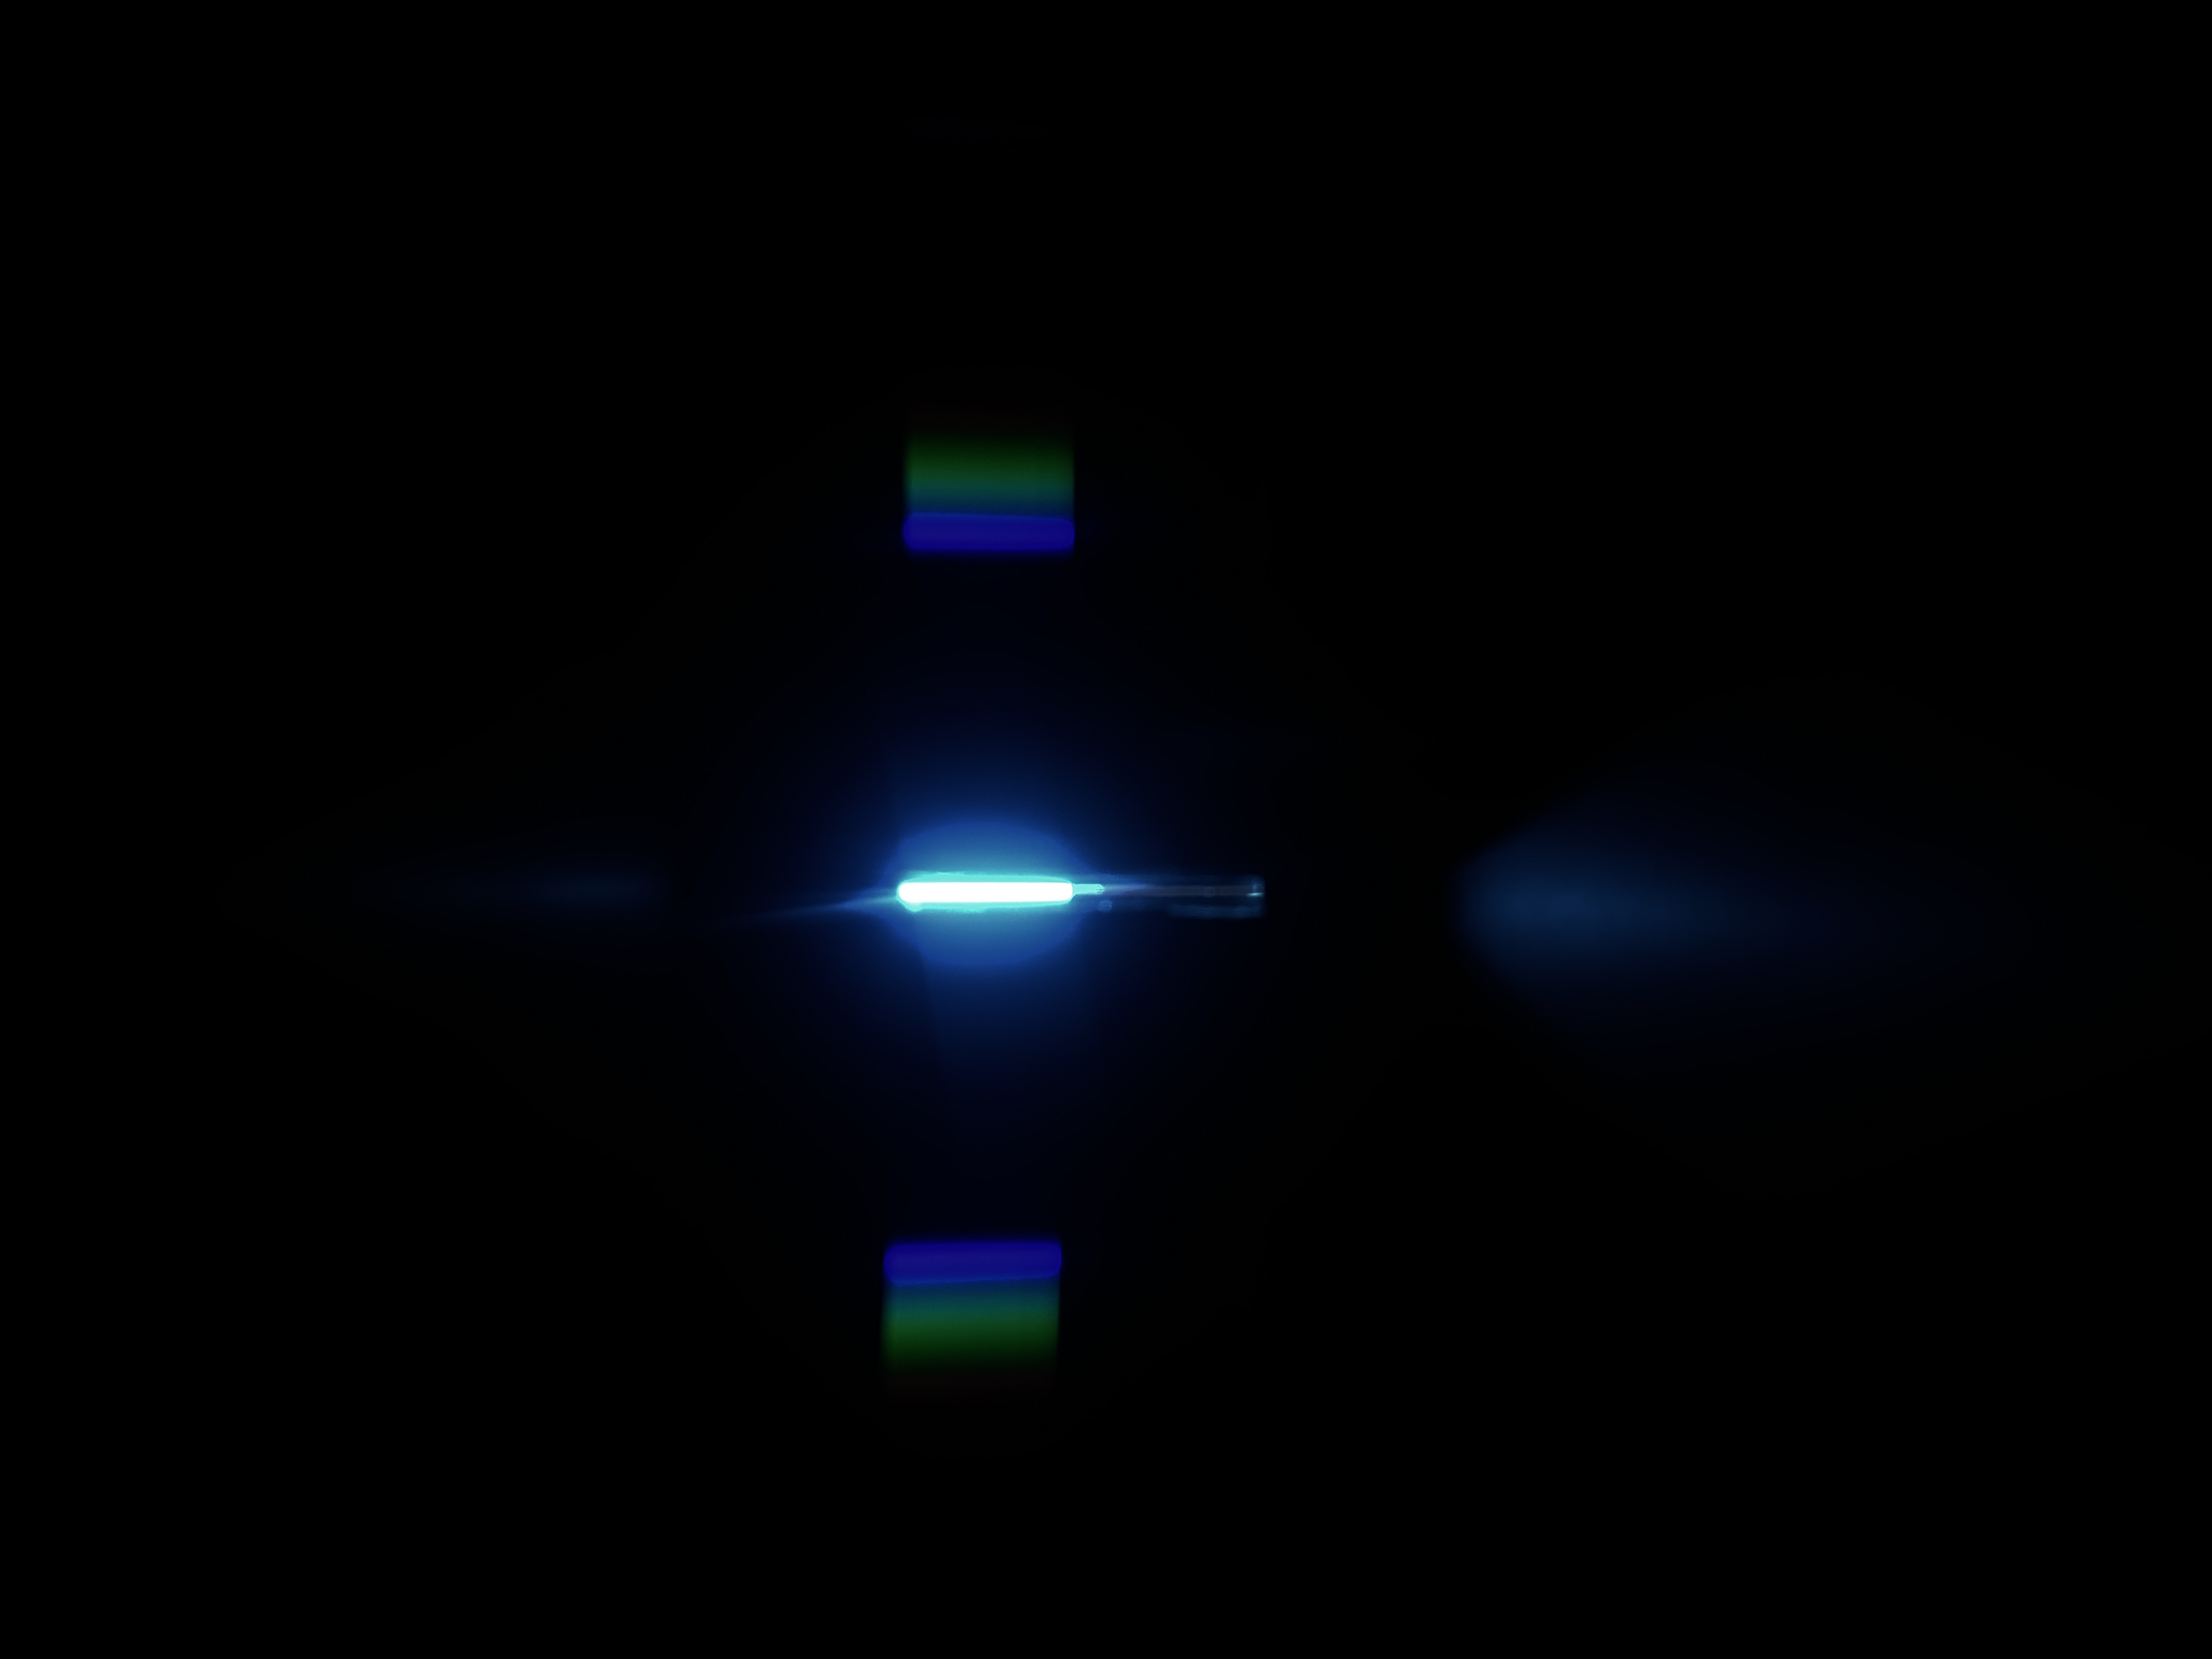
\includegraphics[width=\textwidth]{LED_4.JPG}
            \end{minipage}
            \begin{minipage}{0.45\textwidth}
                \centering
                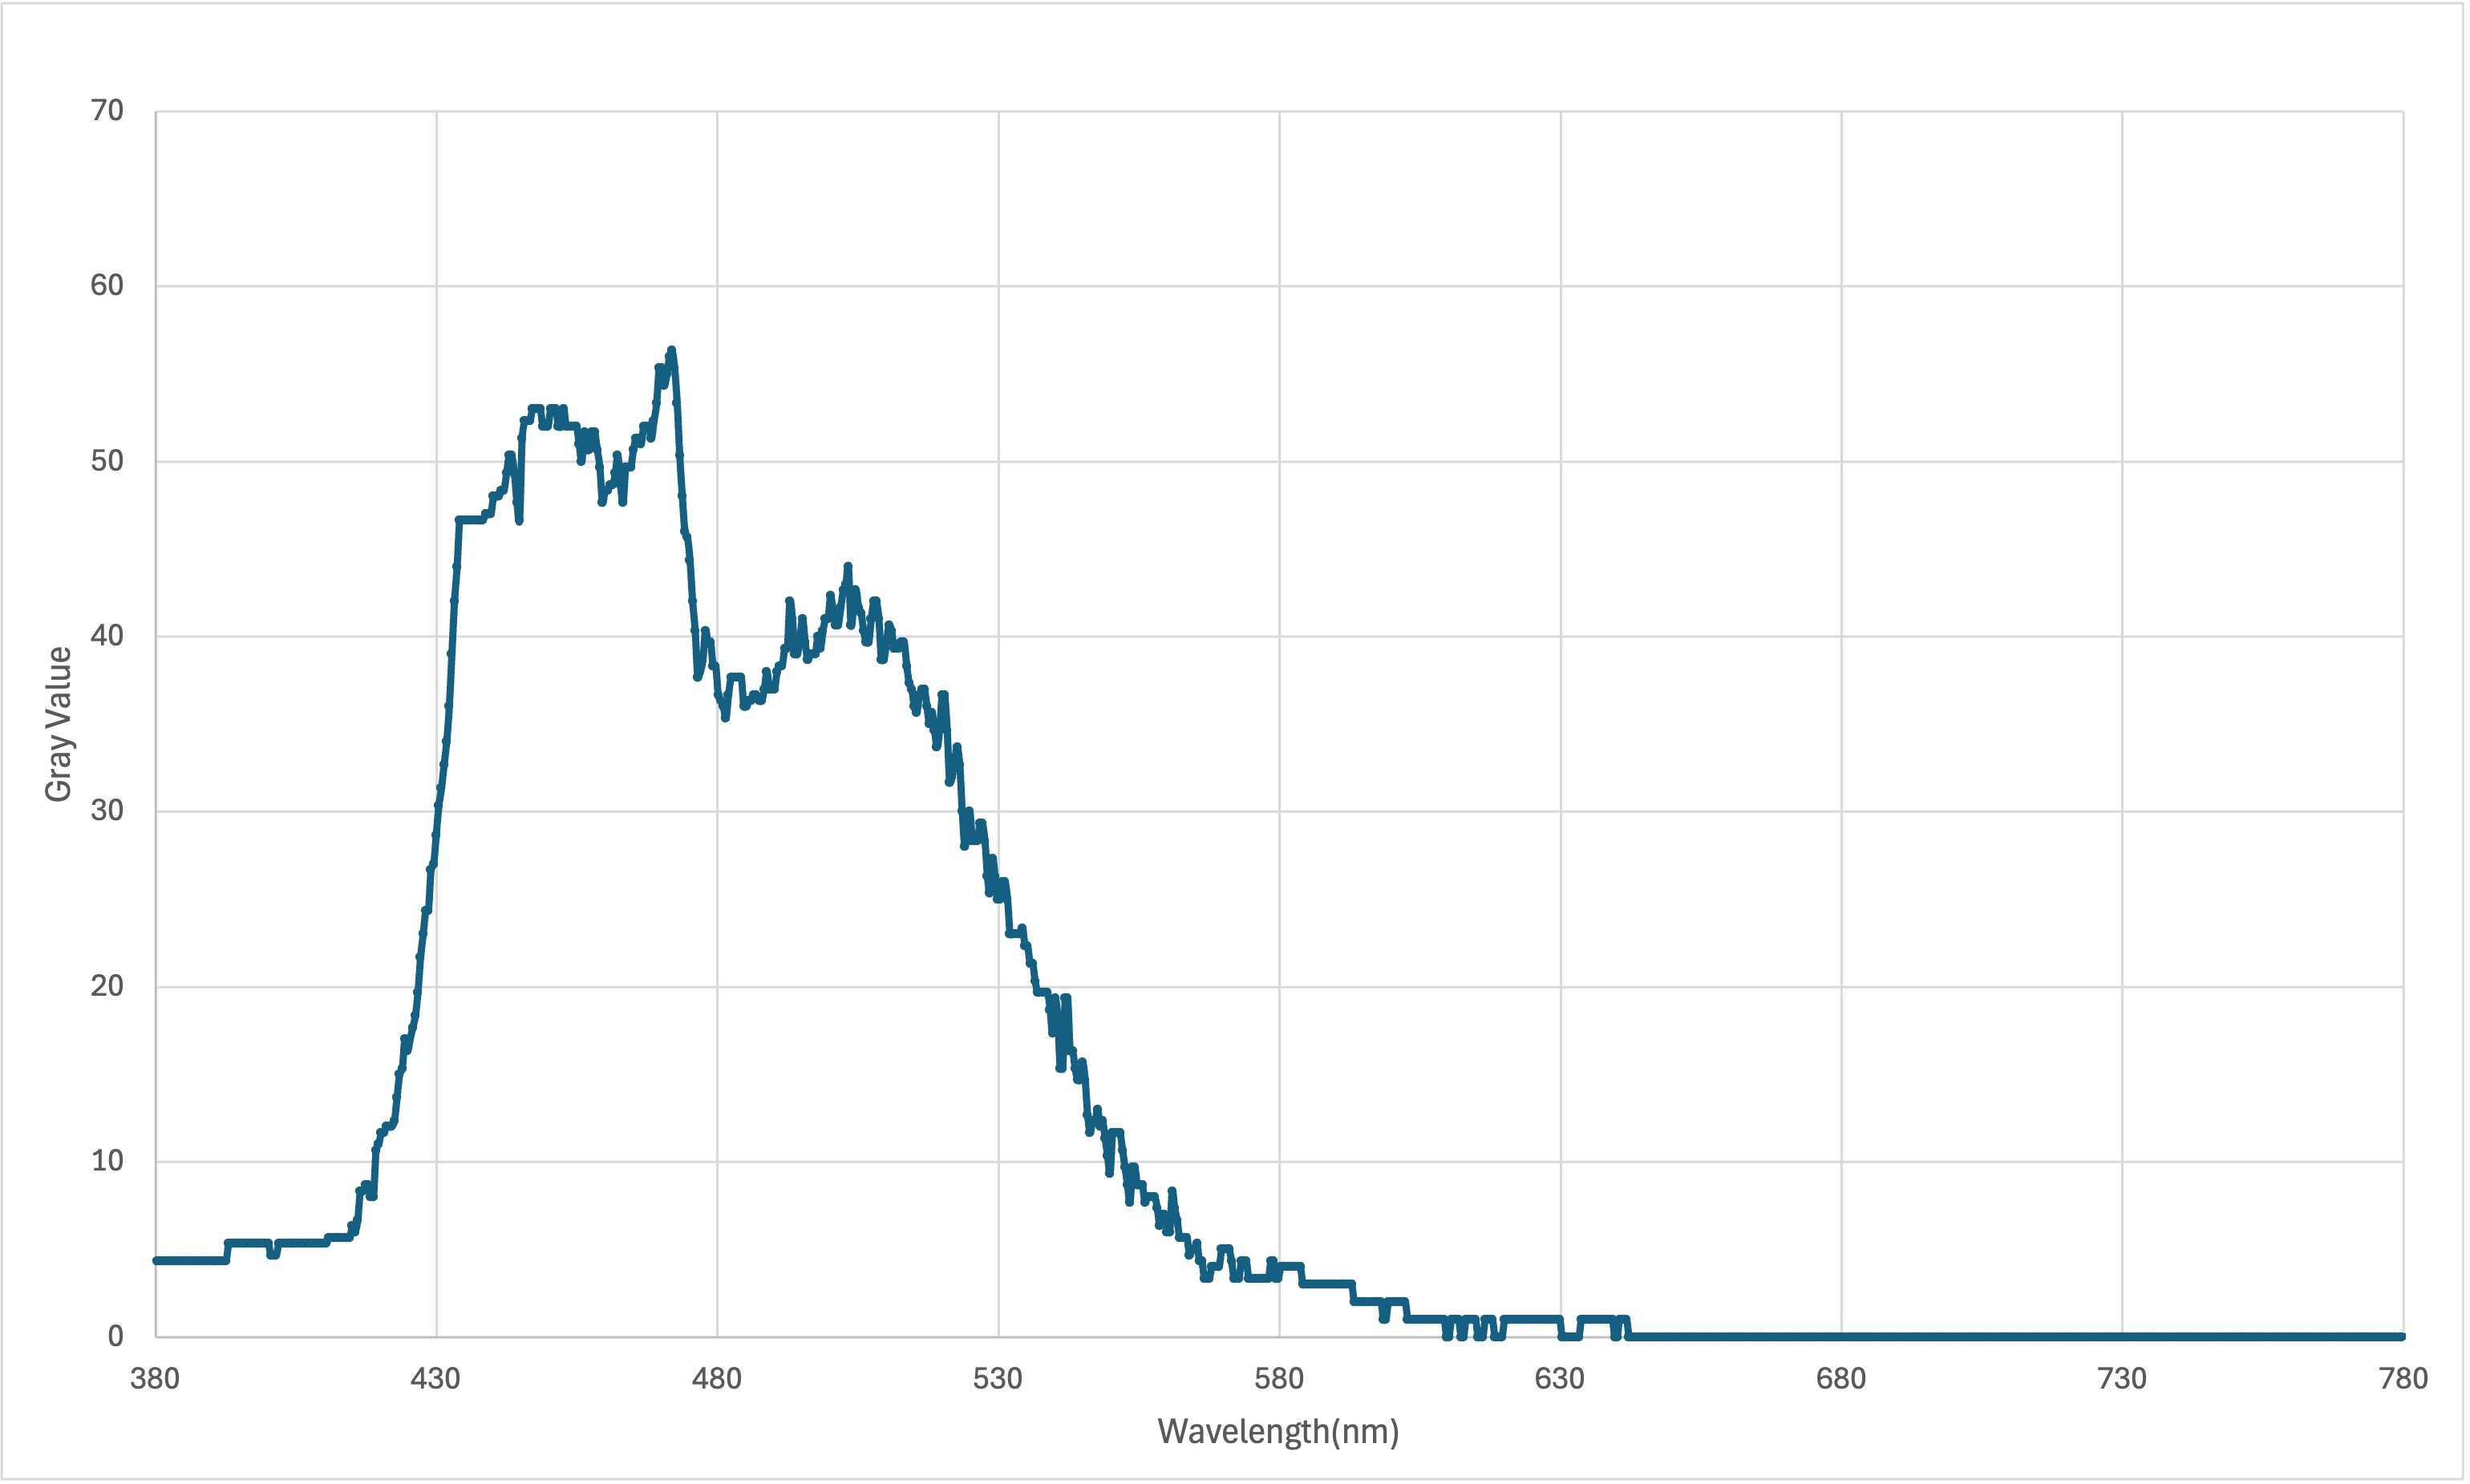
\includegraphics[width=\textwidth]{LED_4S.jpg}
            \end{minipage}
            }
            \caption{LED青光}
        \end{figure}
        
        \begin{figure}[H]
            \centering
            \scalebox{0.85}{
            \begin{minipage}{0.45\textwidth}
                \centering
                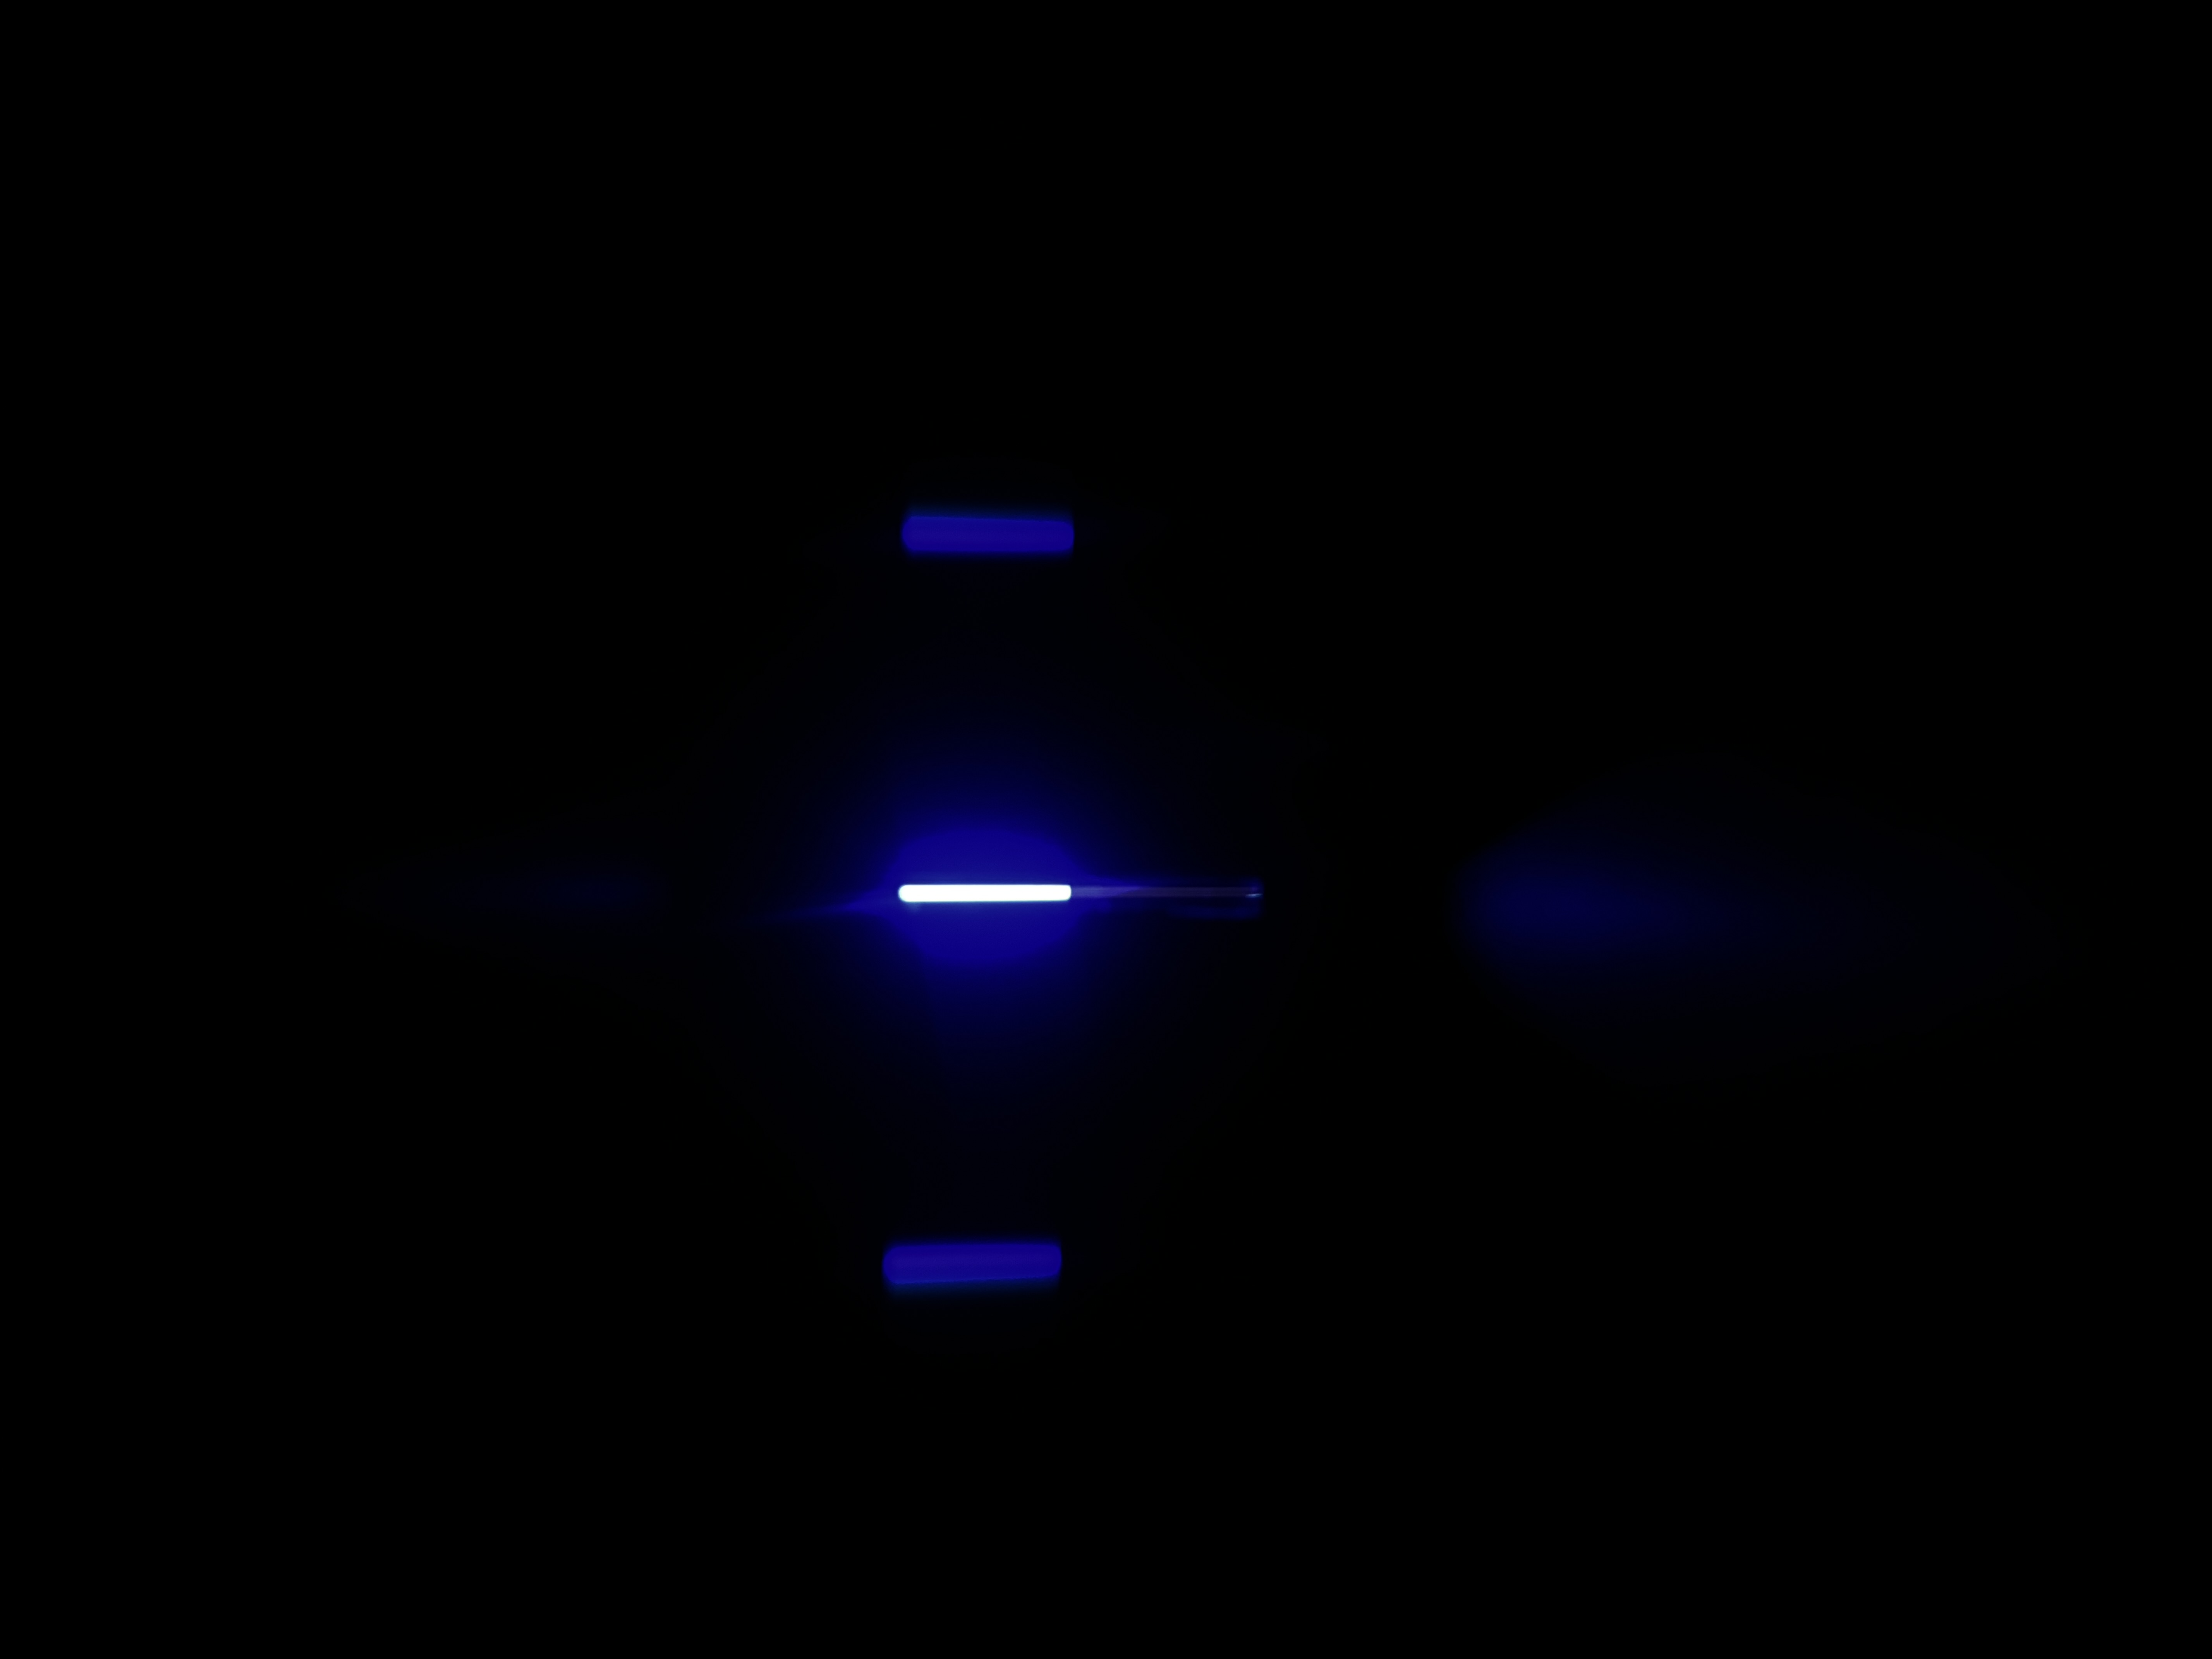
\includegraphics[width=\textwidth]{LED_5.JPG}
            \end{minipage}
            \begin{minipage}{0.45\textwidth}
                \centering
                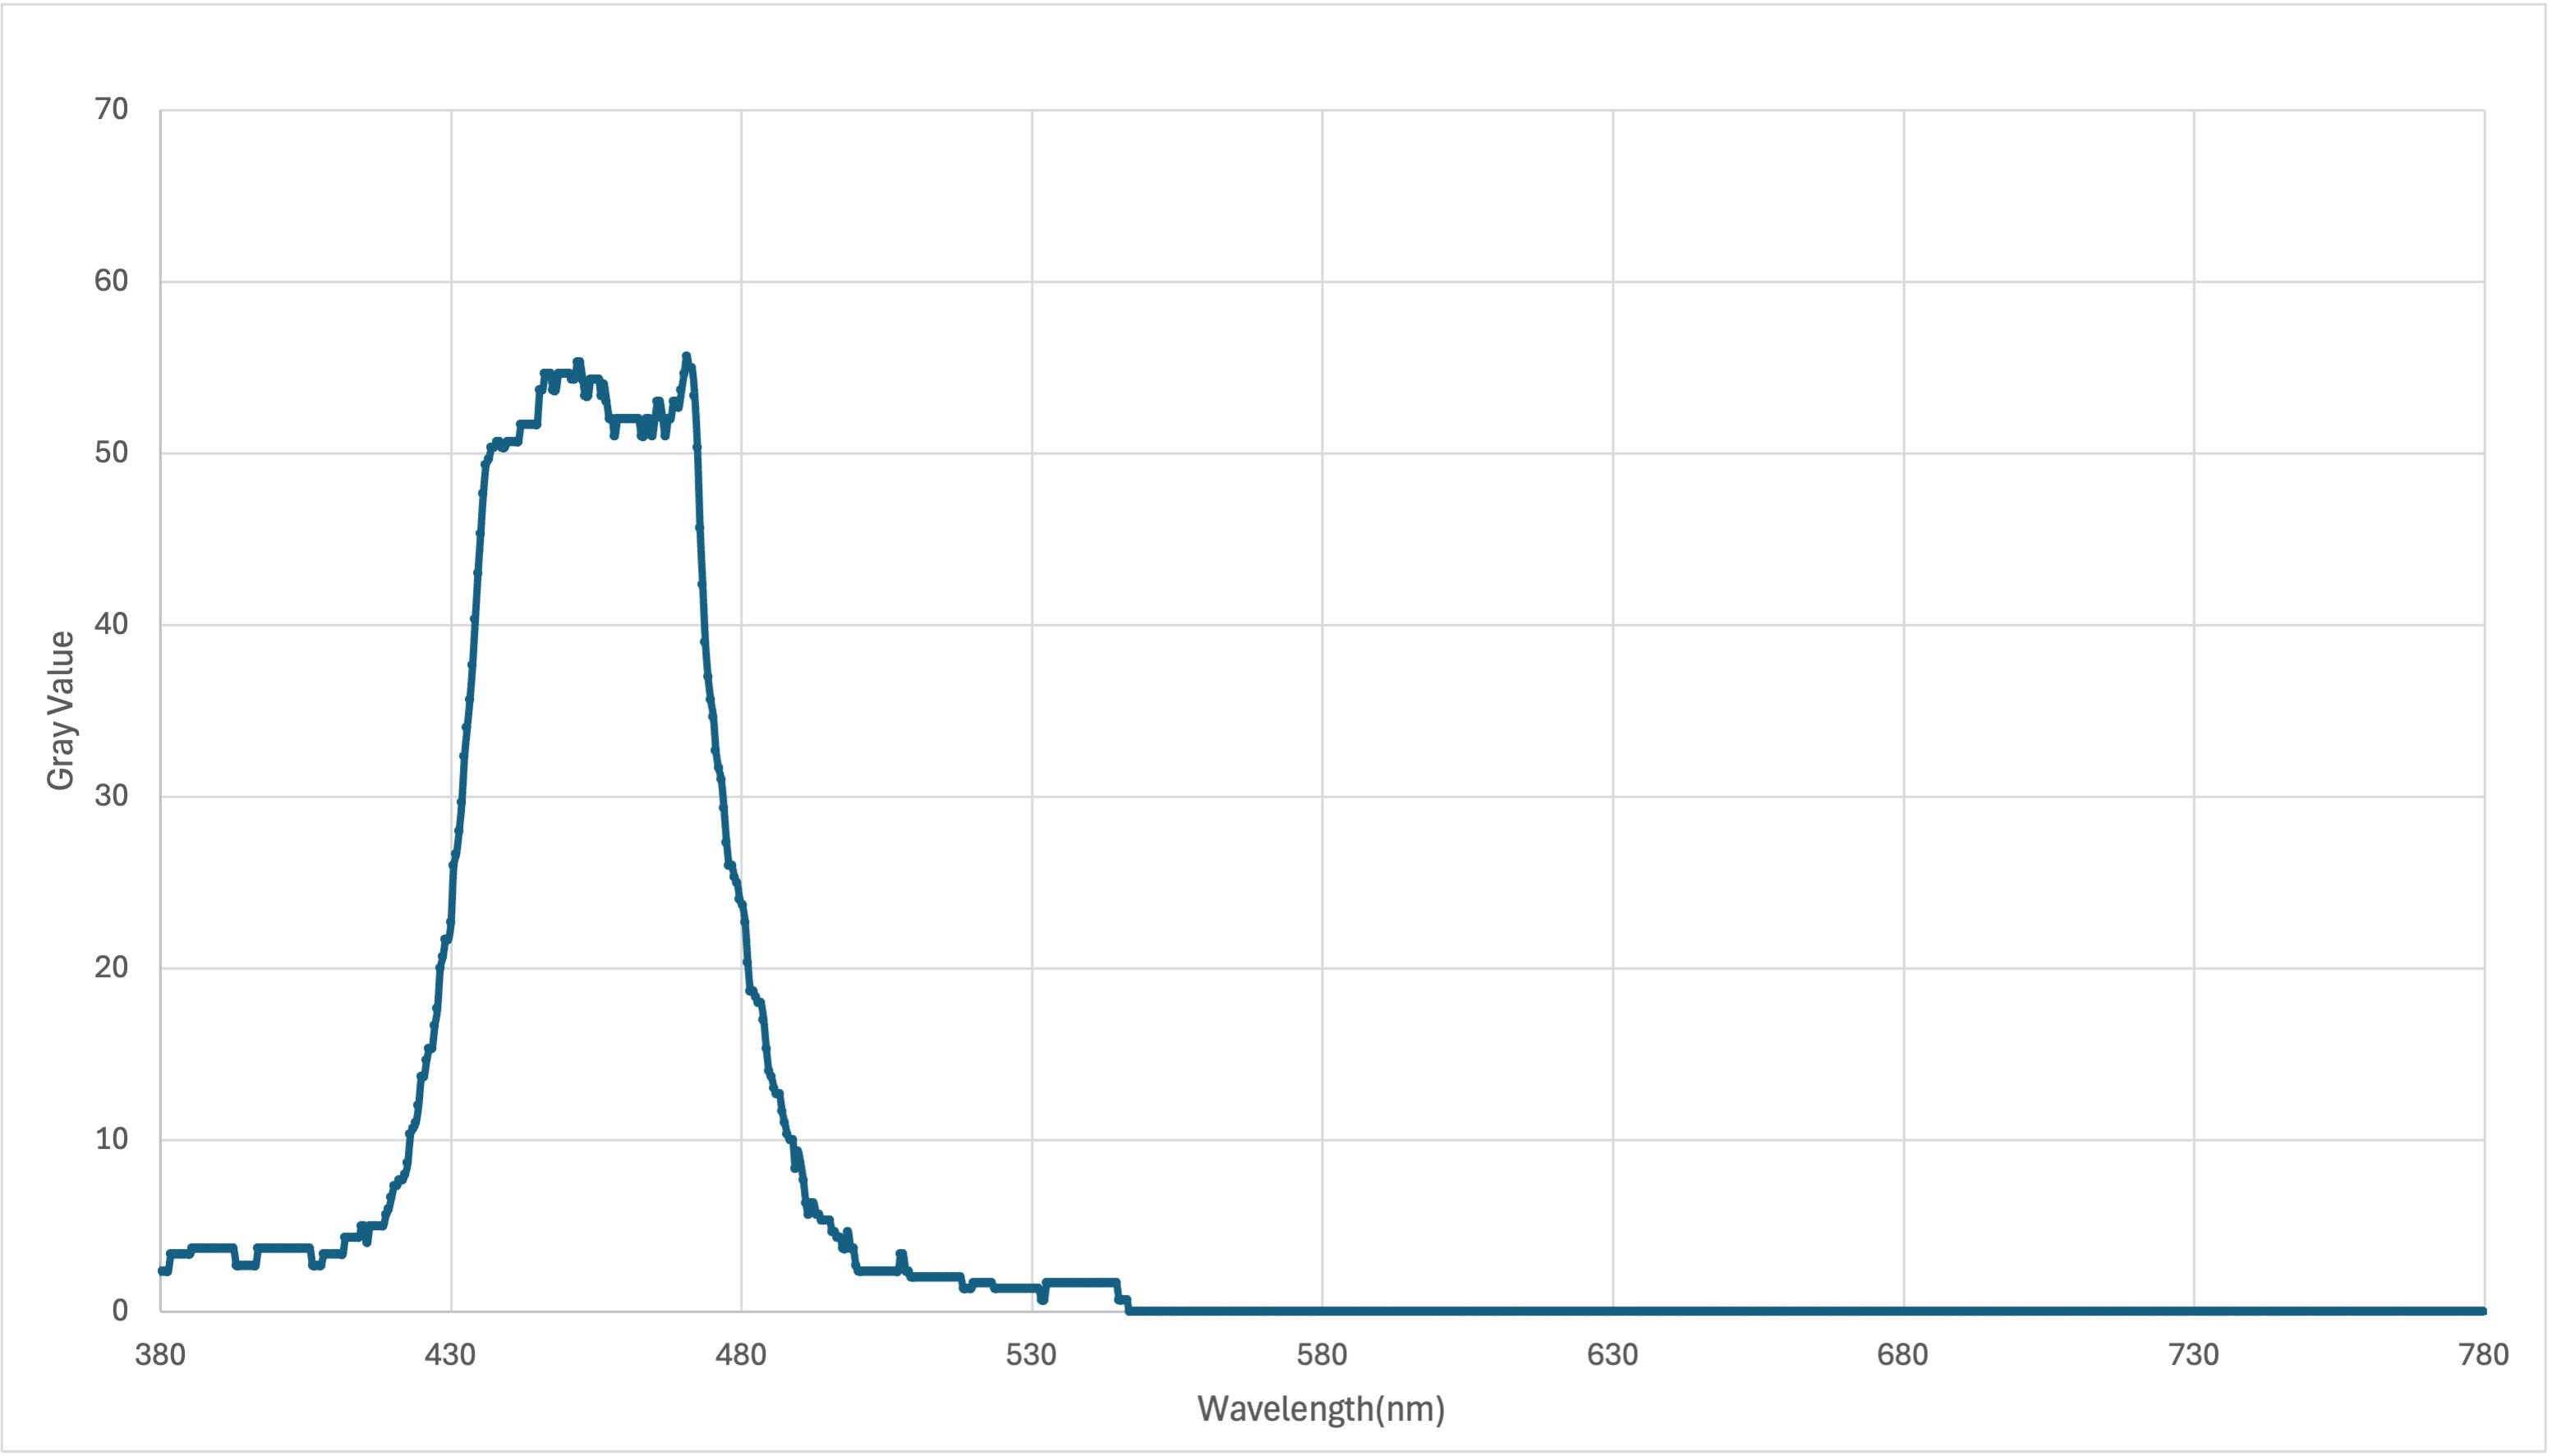
\includegraphics[width=\textwidth]{LED_5S.jpg}
            \end{minipage}
            }
            \caption{LED蓝光}
        \end{figure}

        \begin{figure}[H]
            \centering
            \scalebox{0.85}{
            \begin{minipage}{0.45\textwidth}
                \centering
                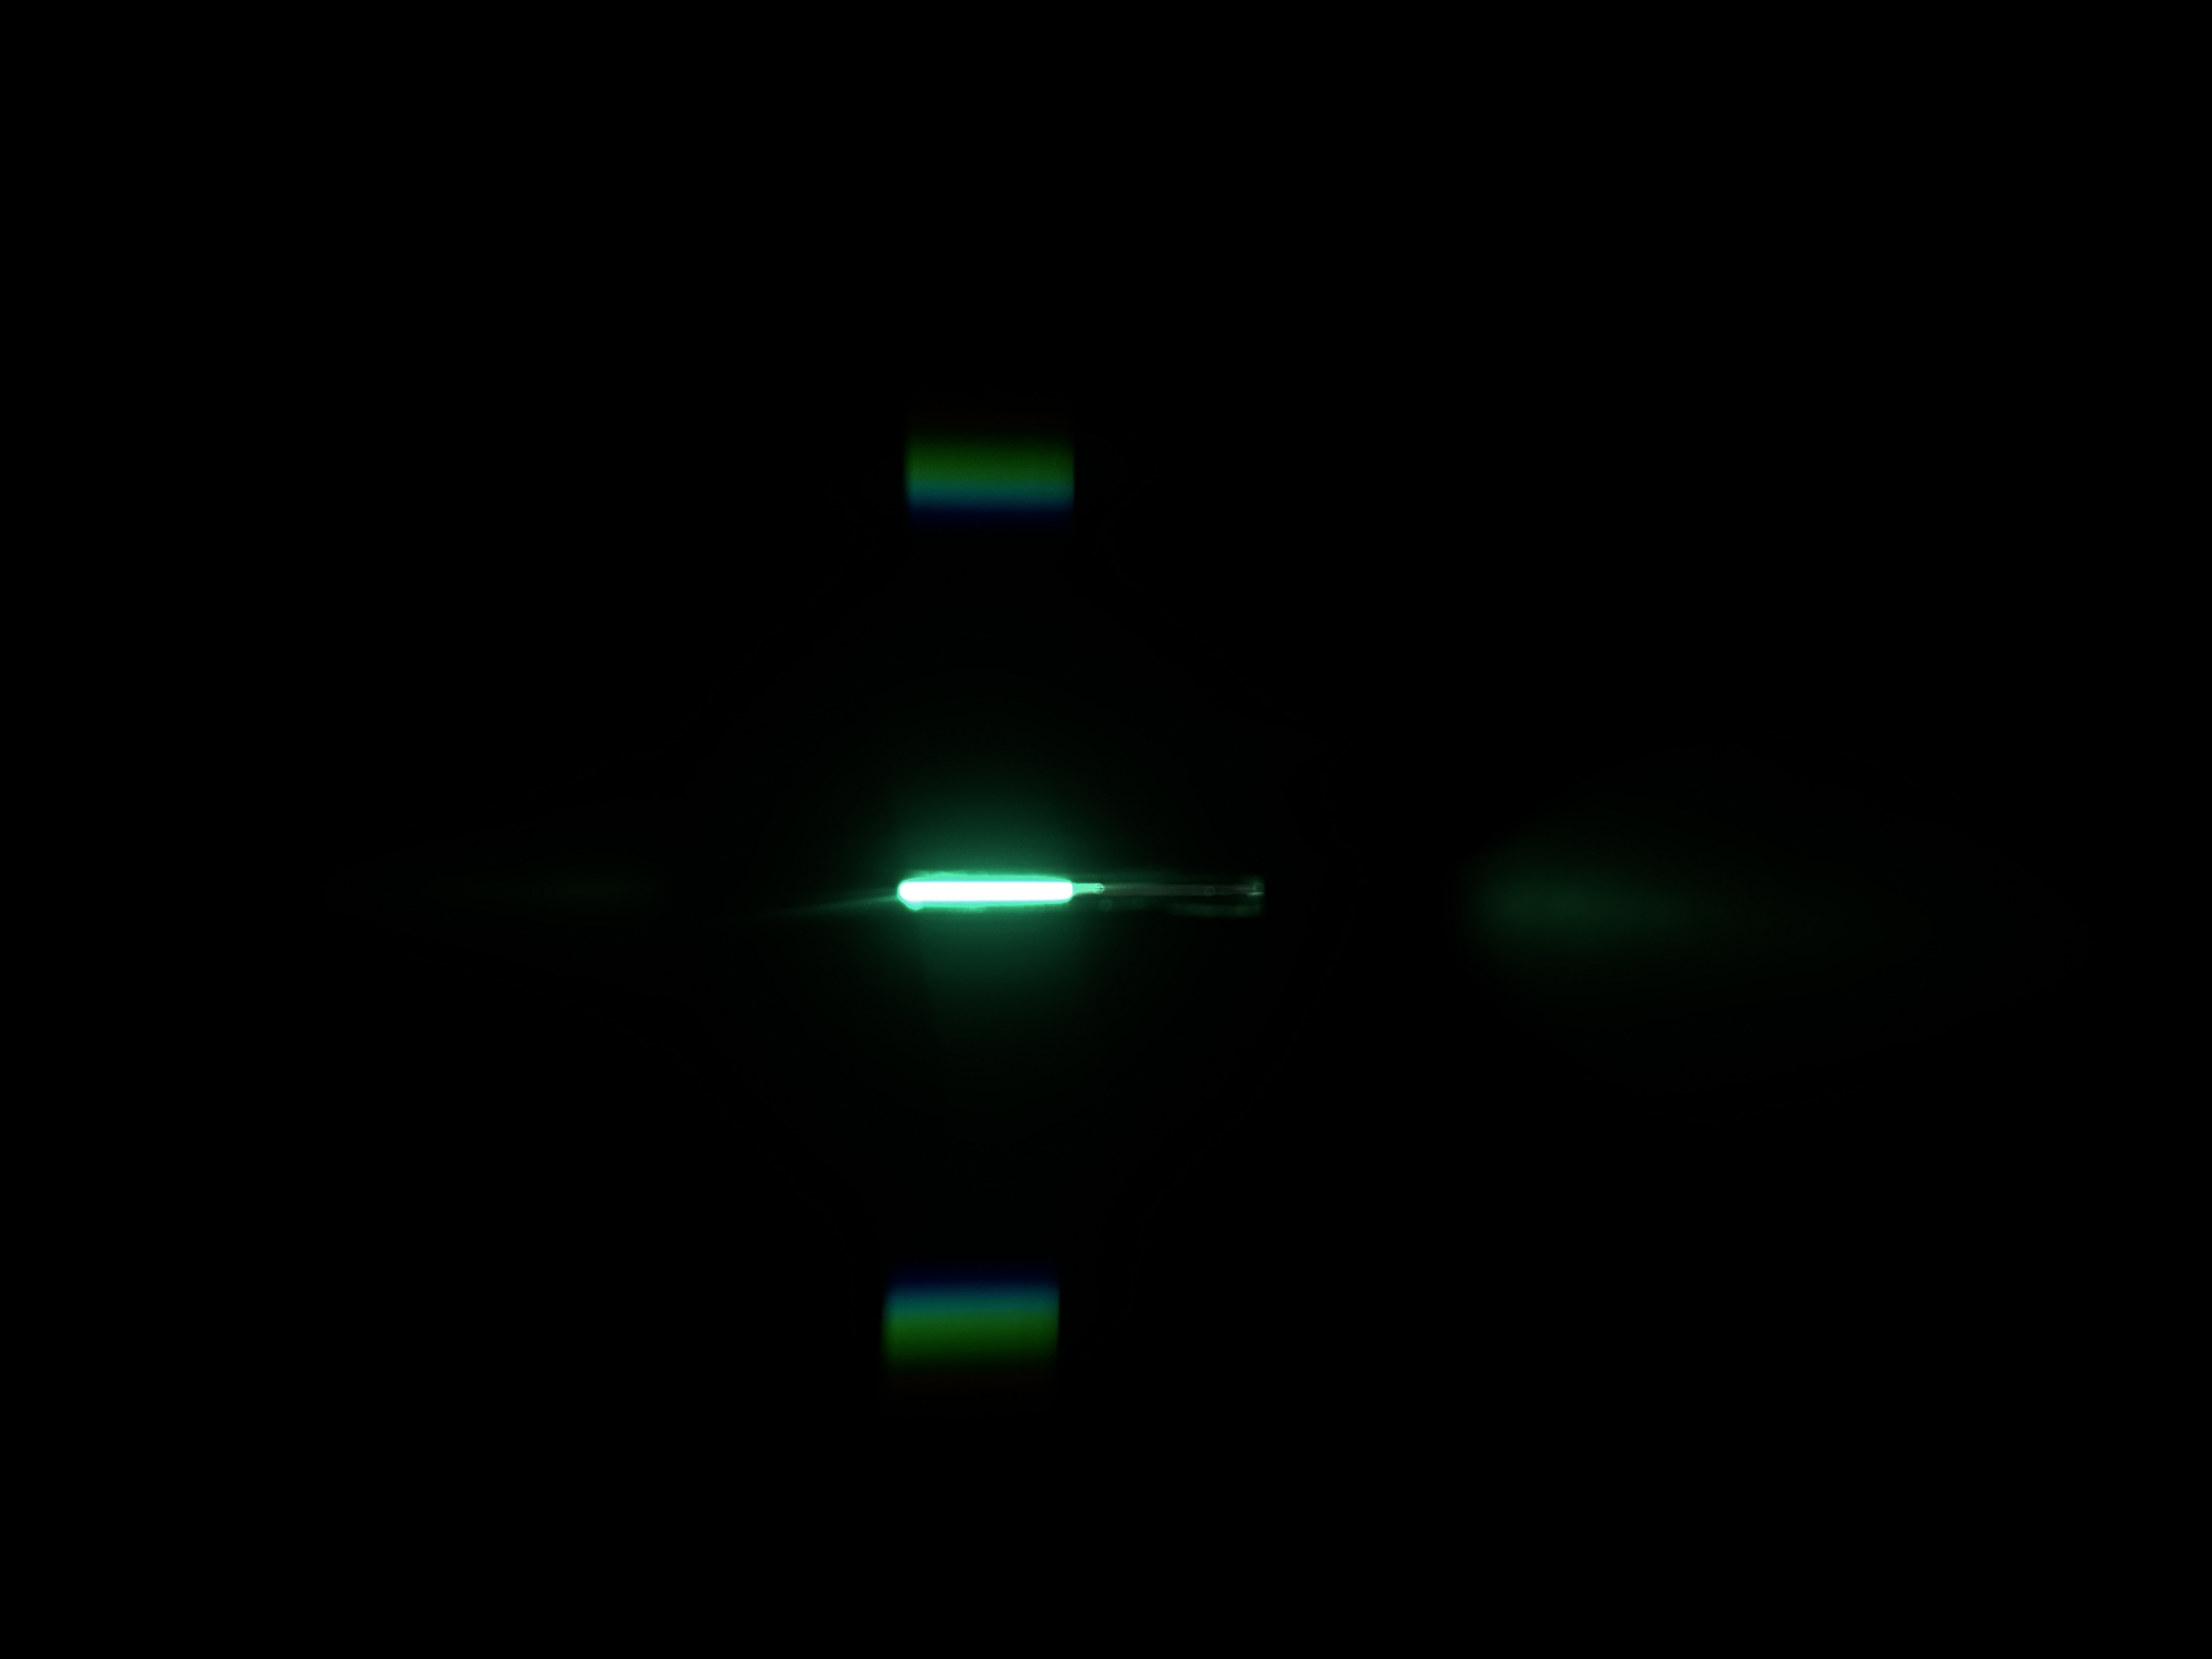
\includegraphics[width=\textwidth]{LED_6.JPG}
            \end{minipage}
            \begin{minipage}{0.45\textwidth}
                \centering
                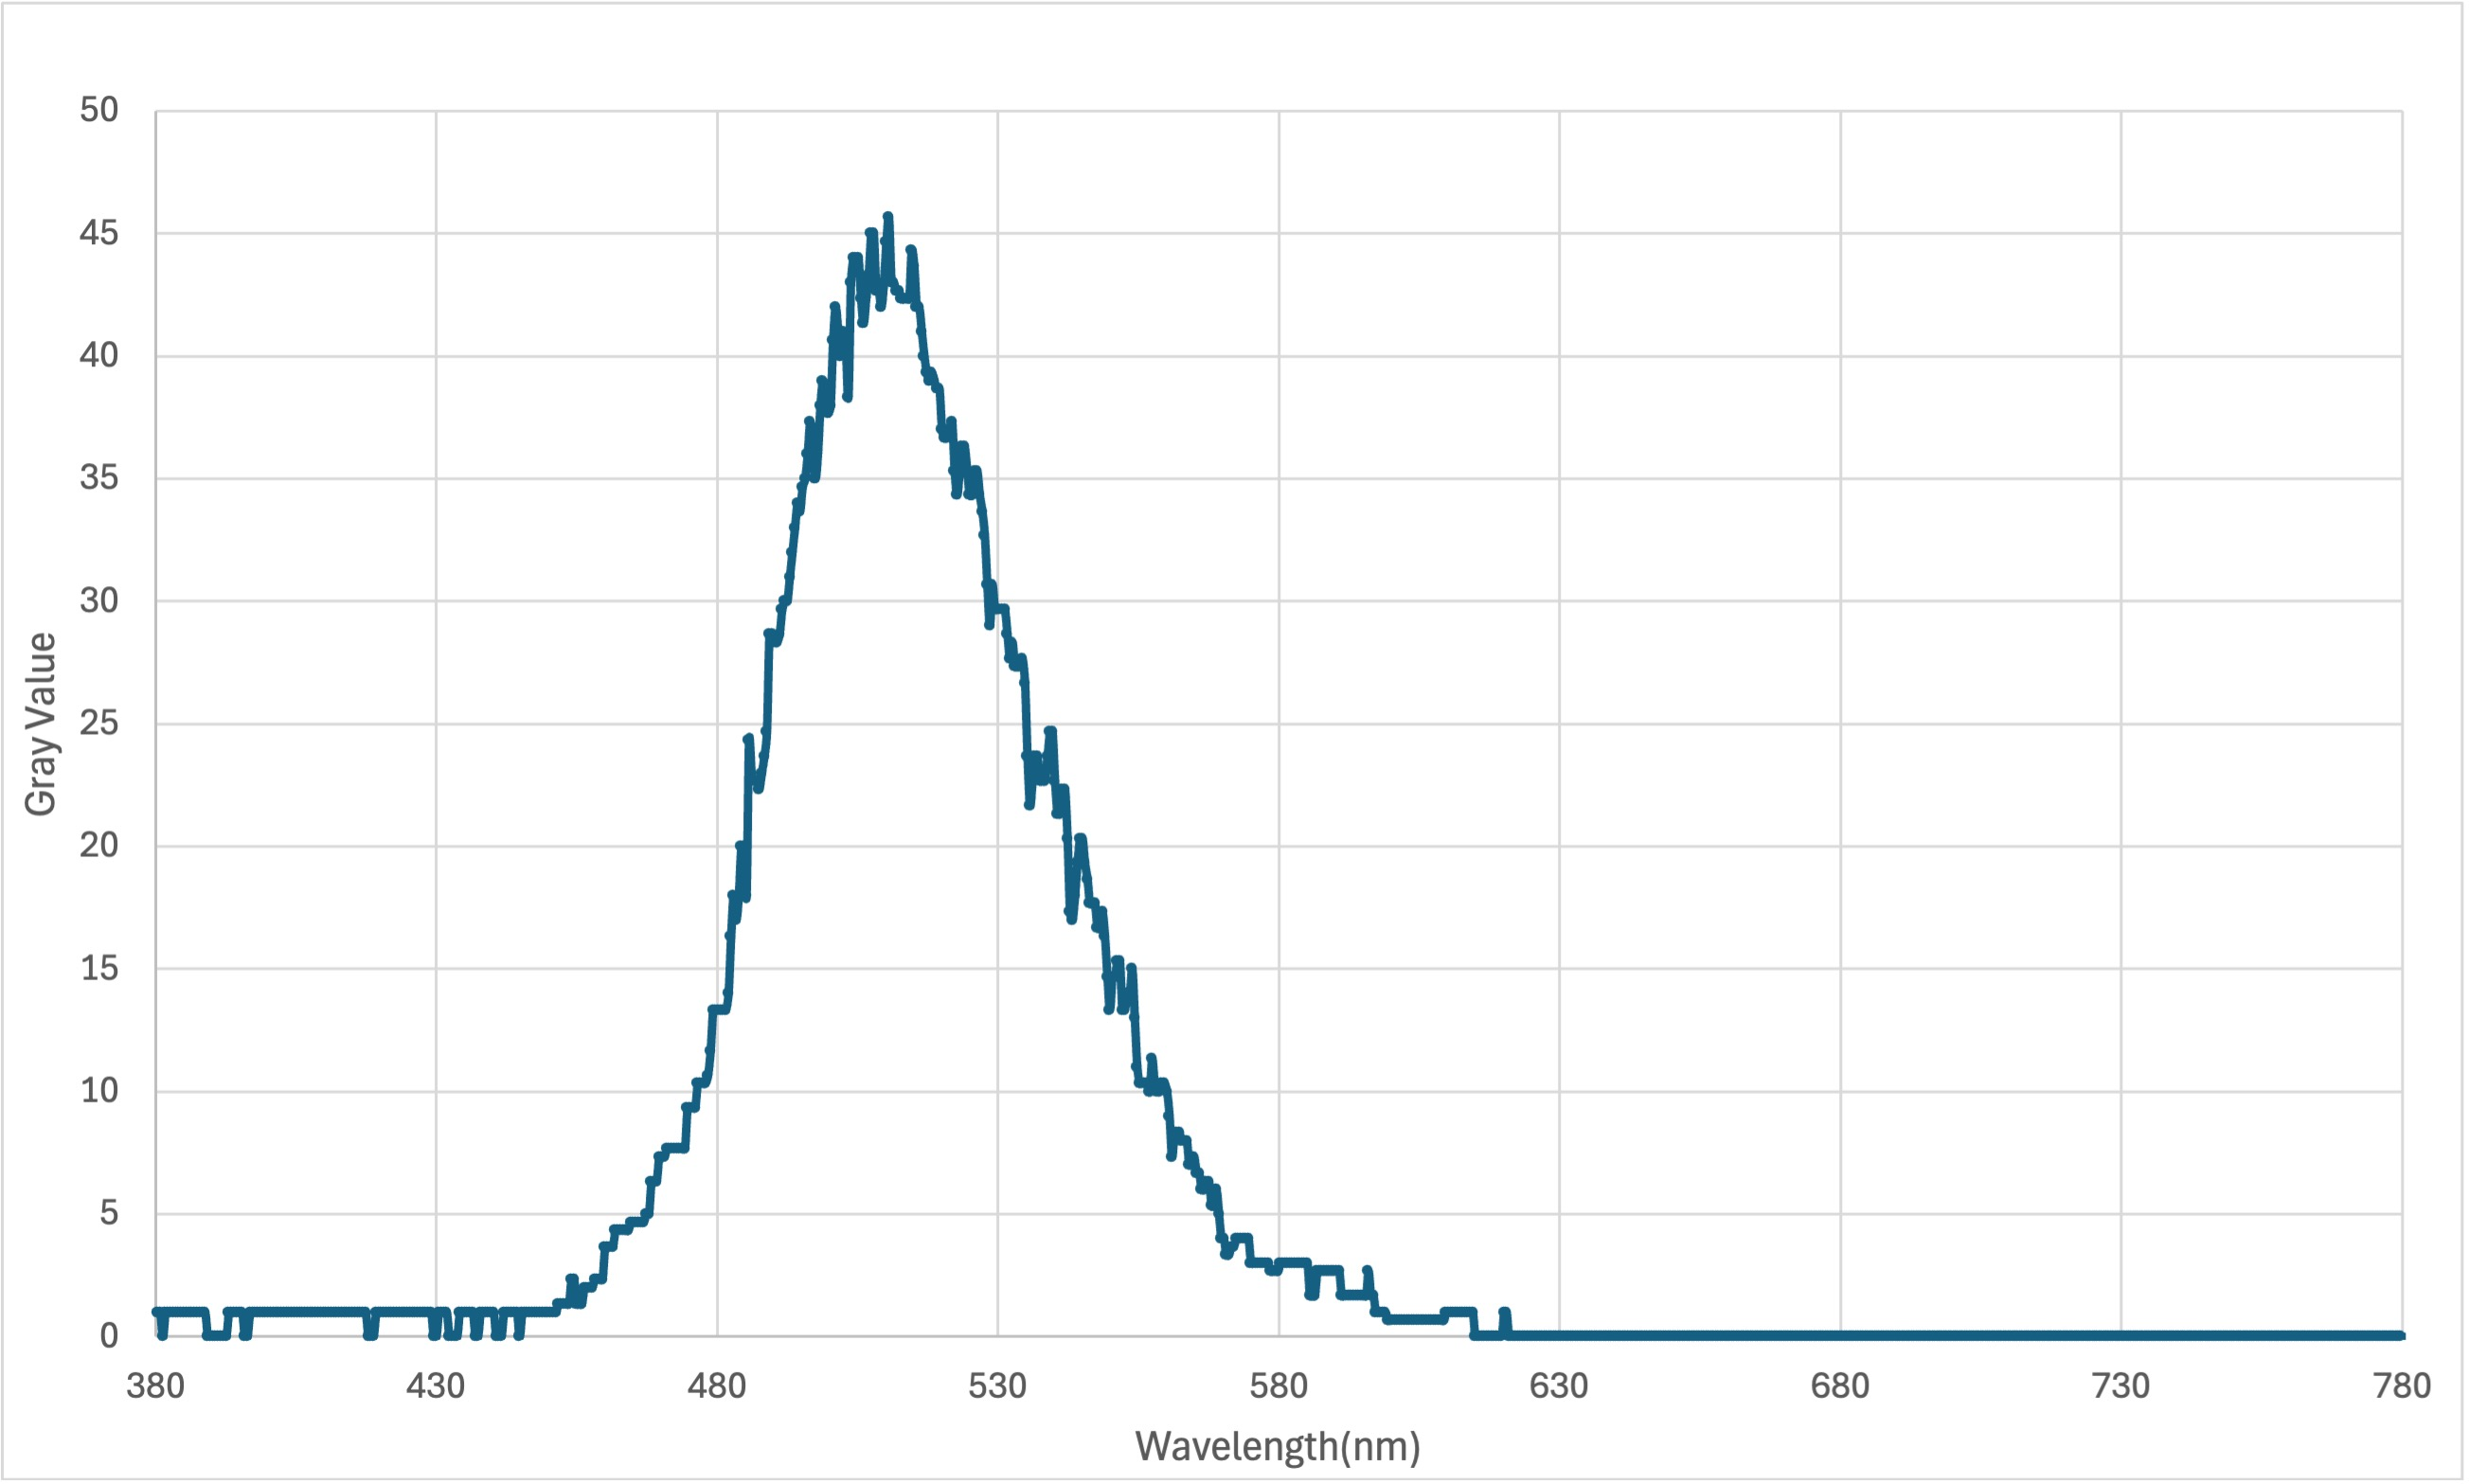
\includegraphics[width=\textwidth]{LED_6S.jpg}
            \end{minipage}
            }
            \caption{LED绿光}
        \end{figure}

        \begin{figure}[H]
            \centering
            \scalebox{0.85}{
            \begin{minipage}{0.45\textwidth}
                \centering
                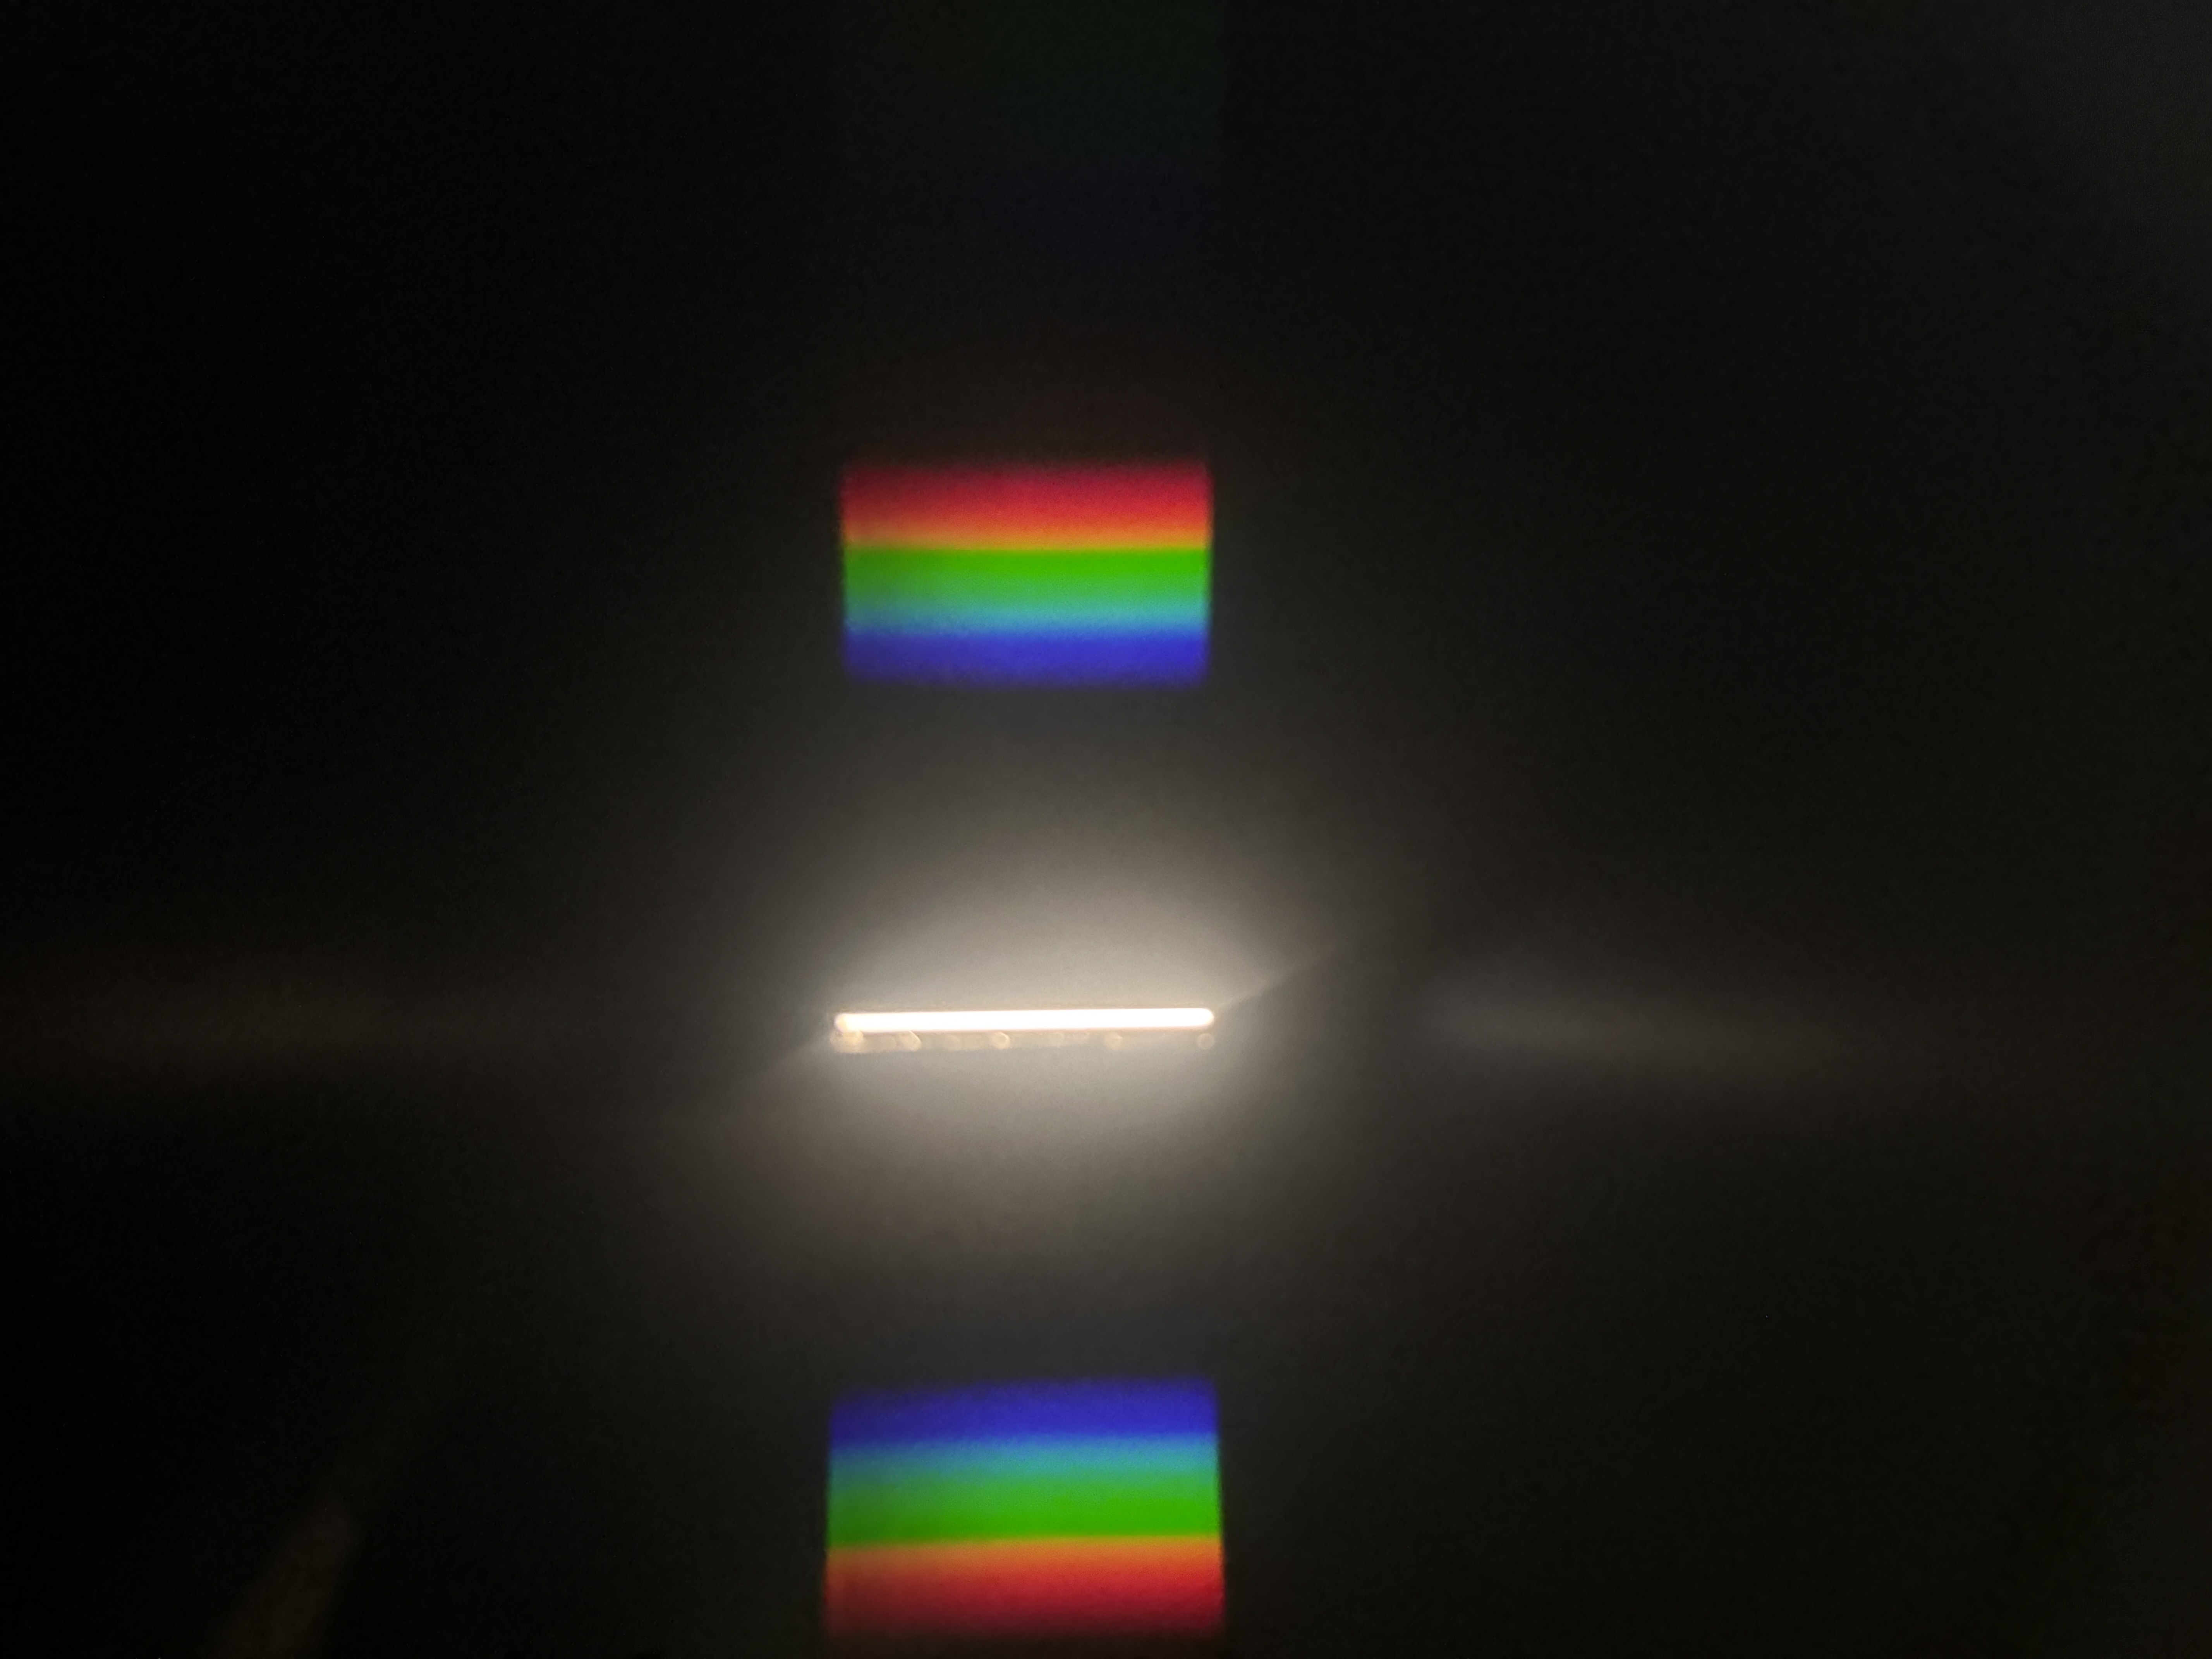
\includegraphics[width=\textwidth]{Incandescent Light.JPG}
            \end{minipage}
            \begin{minipage}{0.45\textwidth}
                \centering
                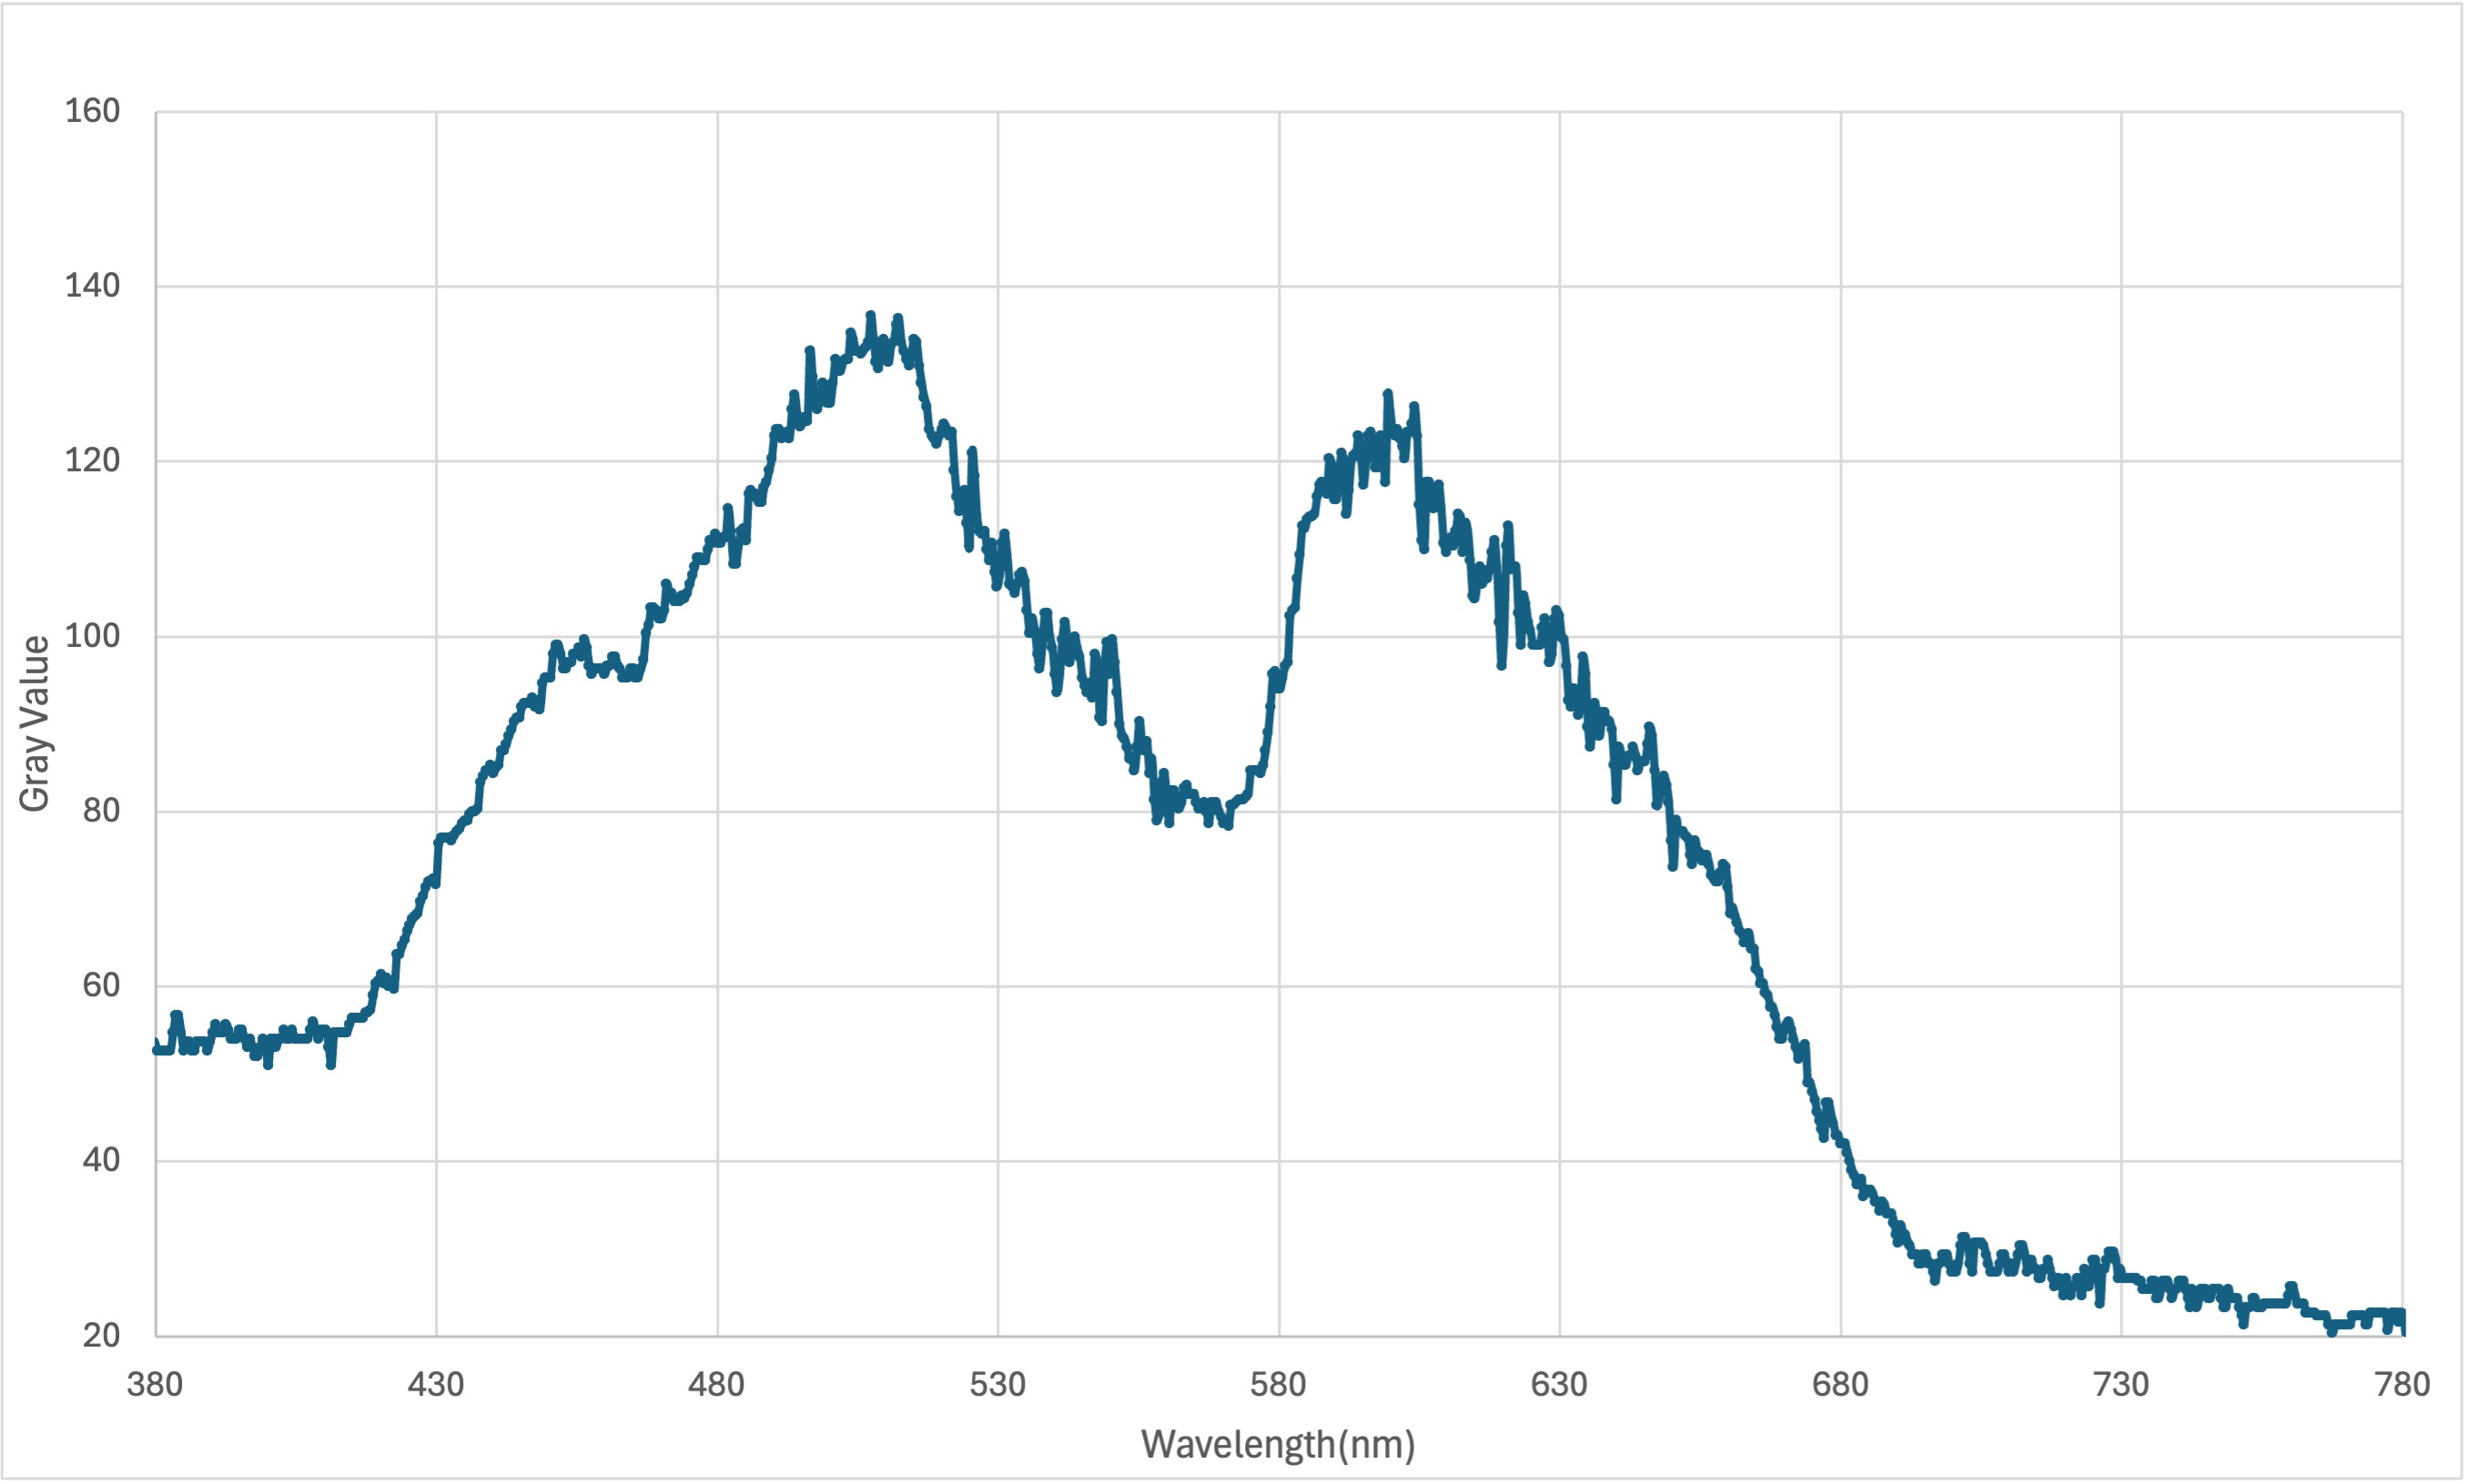
\includegraphics[width=\textwidth]{Incandescent Light_S.jpg}
            \end{minipage}
            }
            \caption{白炽灯}
        \end{figure}

        \begin{figure}[H]
            \centering
            \scalebox{0.85}{
            \begin{minipage}{0.45\textwidth}
                \centering
                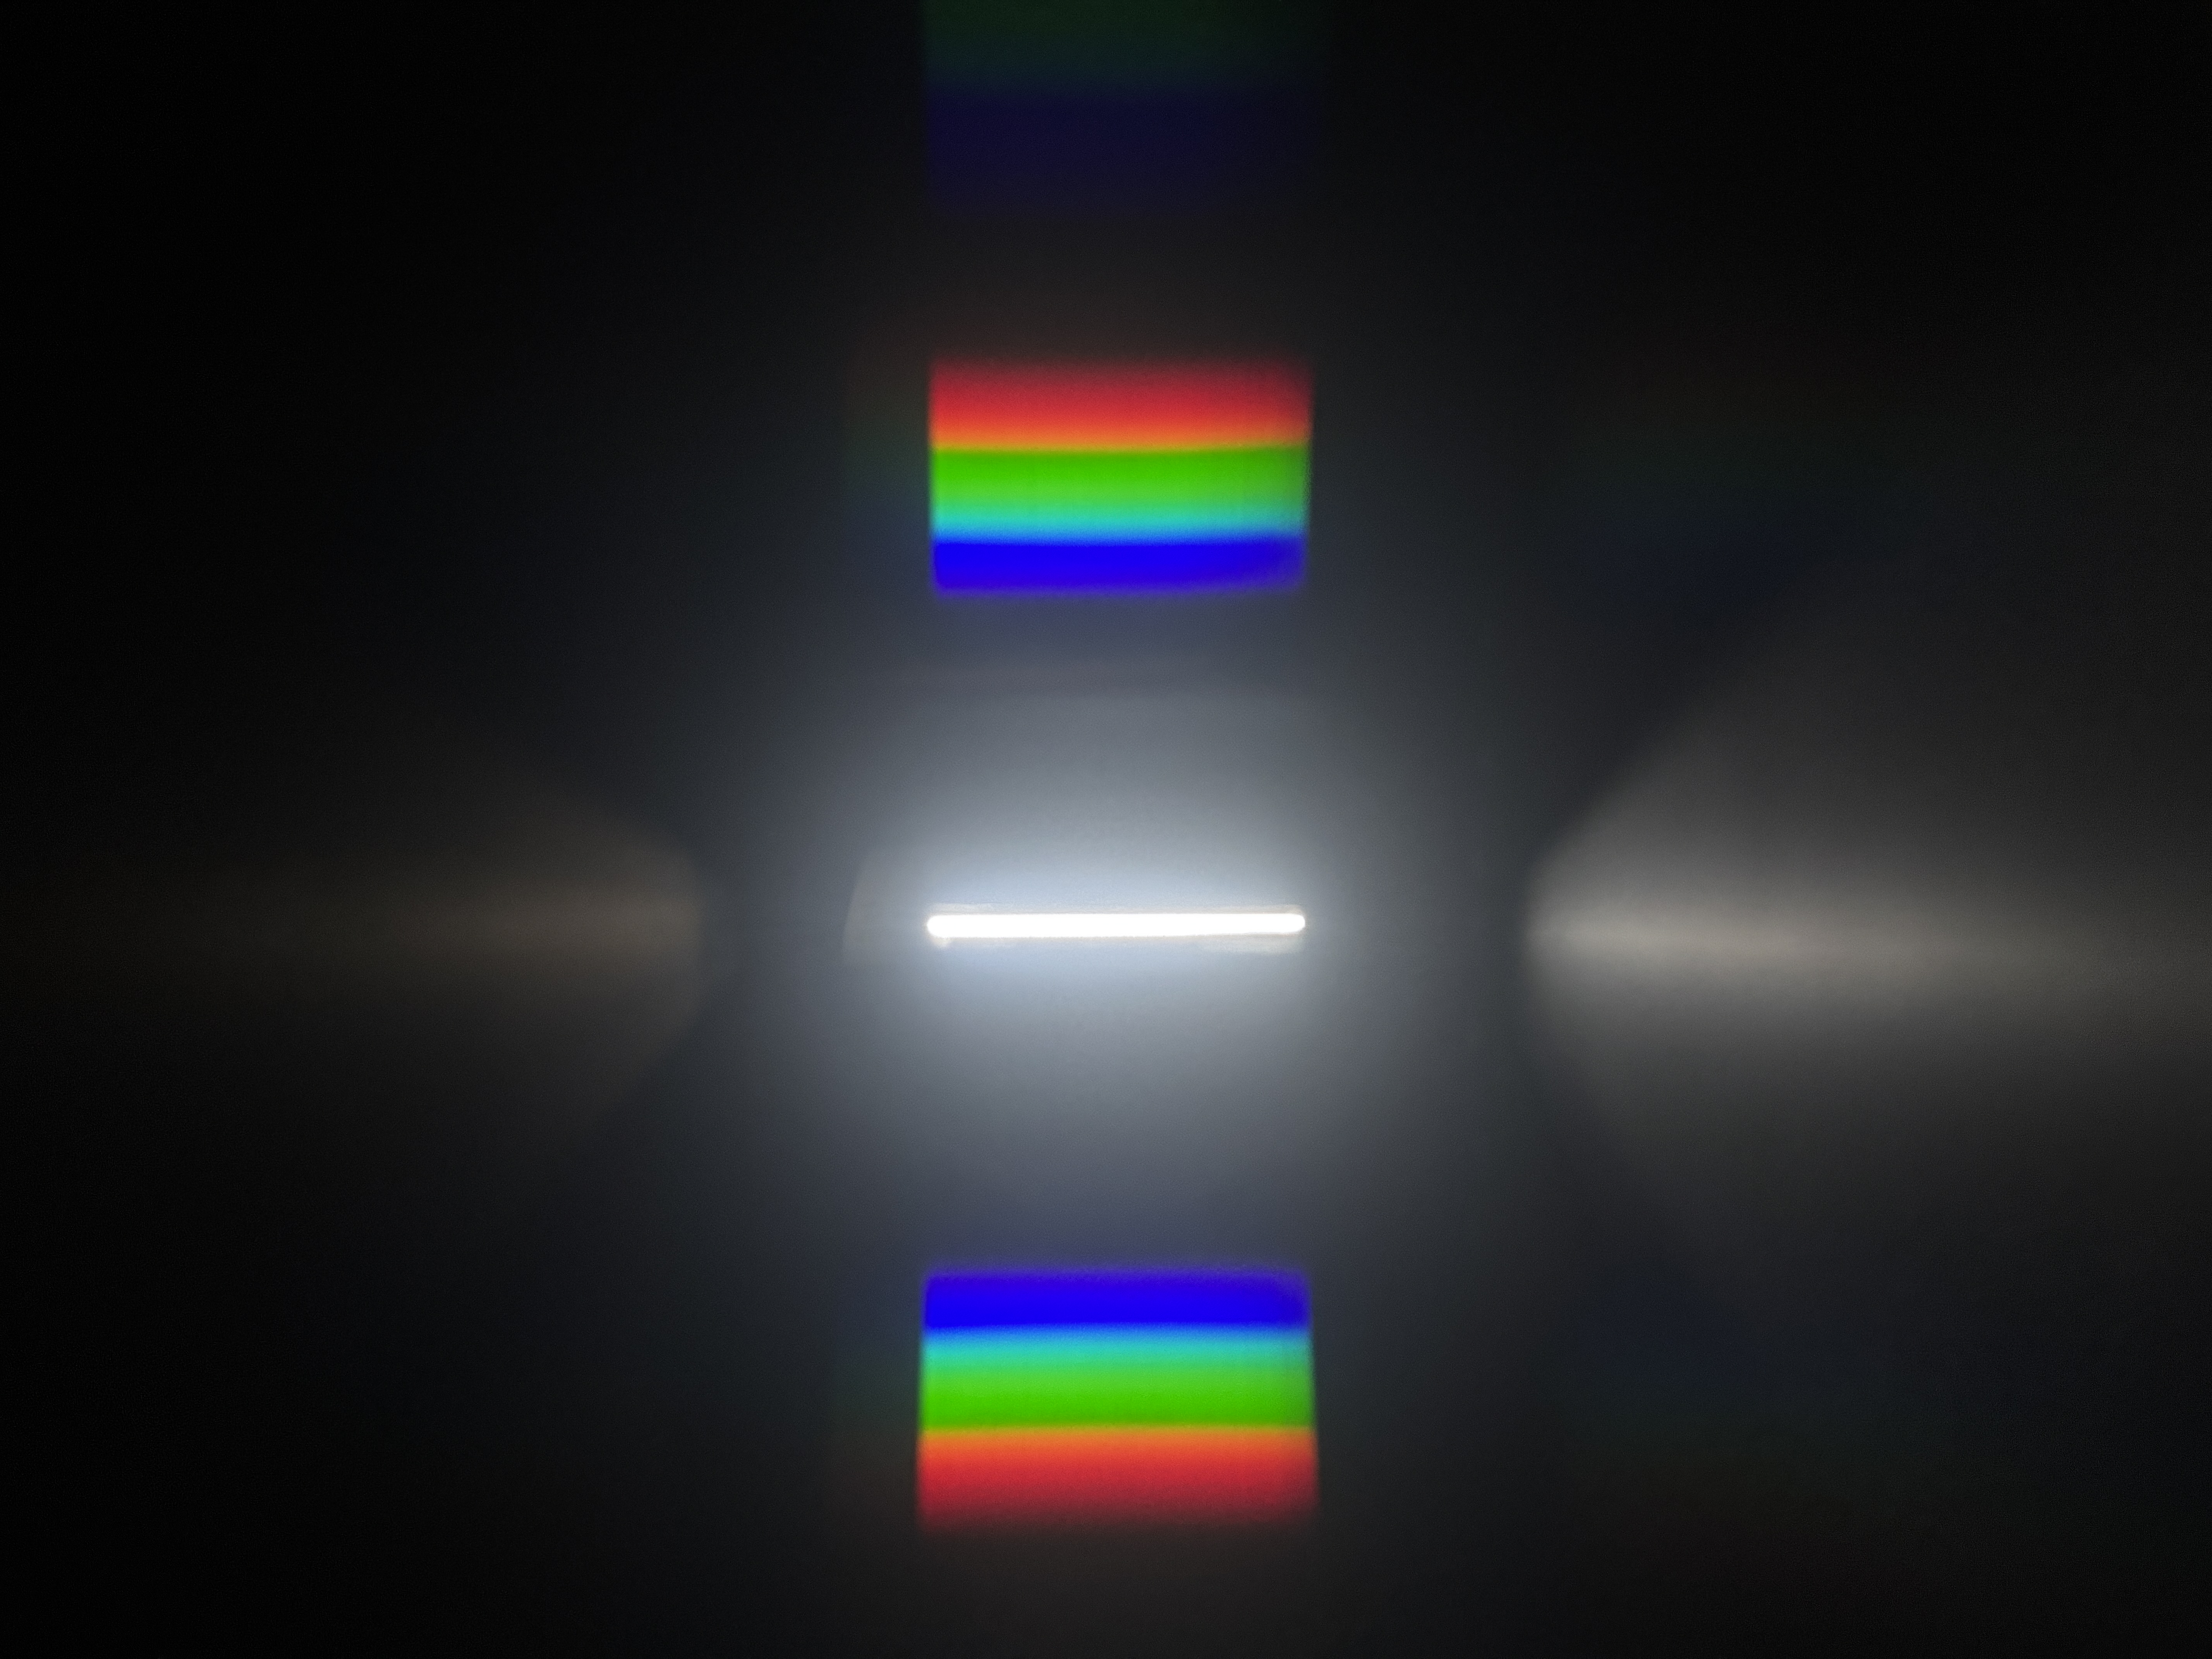
\includegraphics[width=\textwidth]{Sunlight.JPG}
            \end{minipage}
            \begin{minipage}{0.45\textwidth}
                \centering
                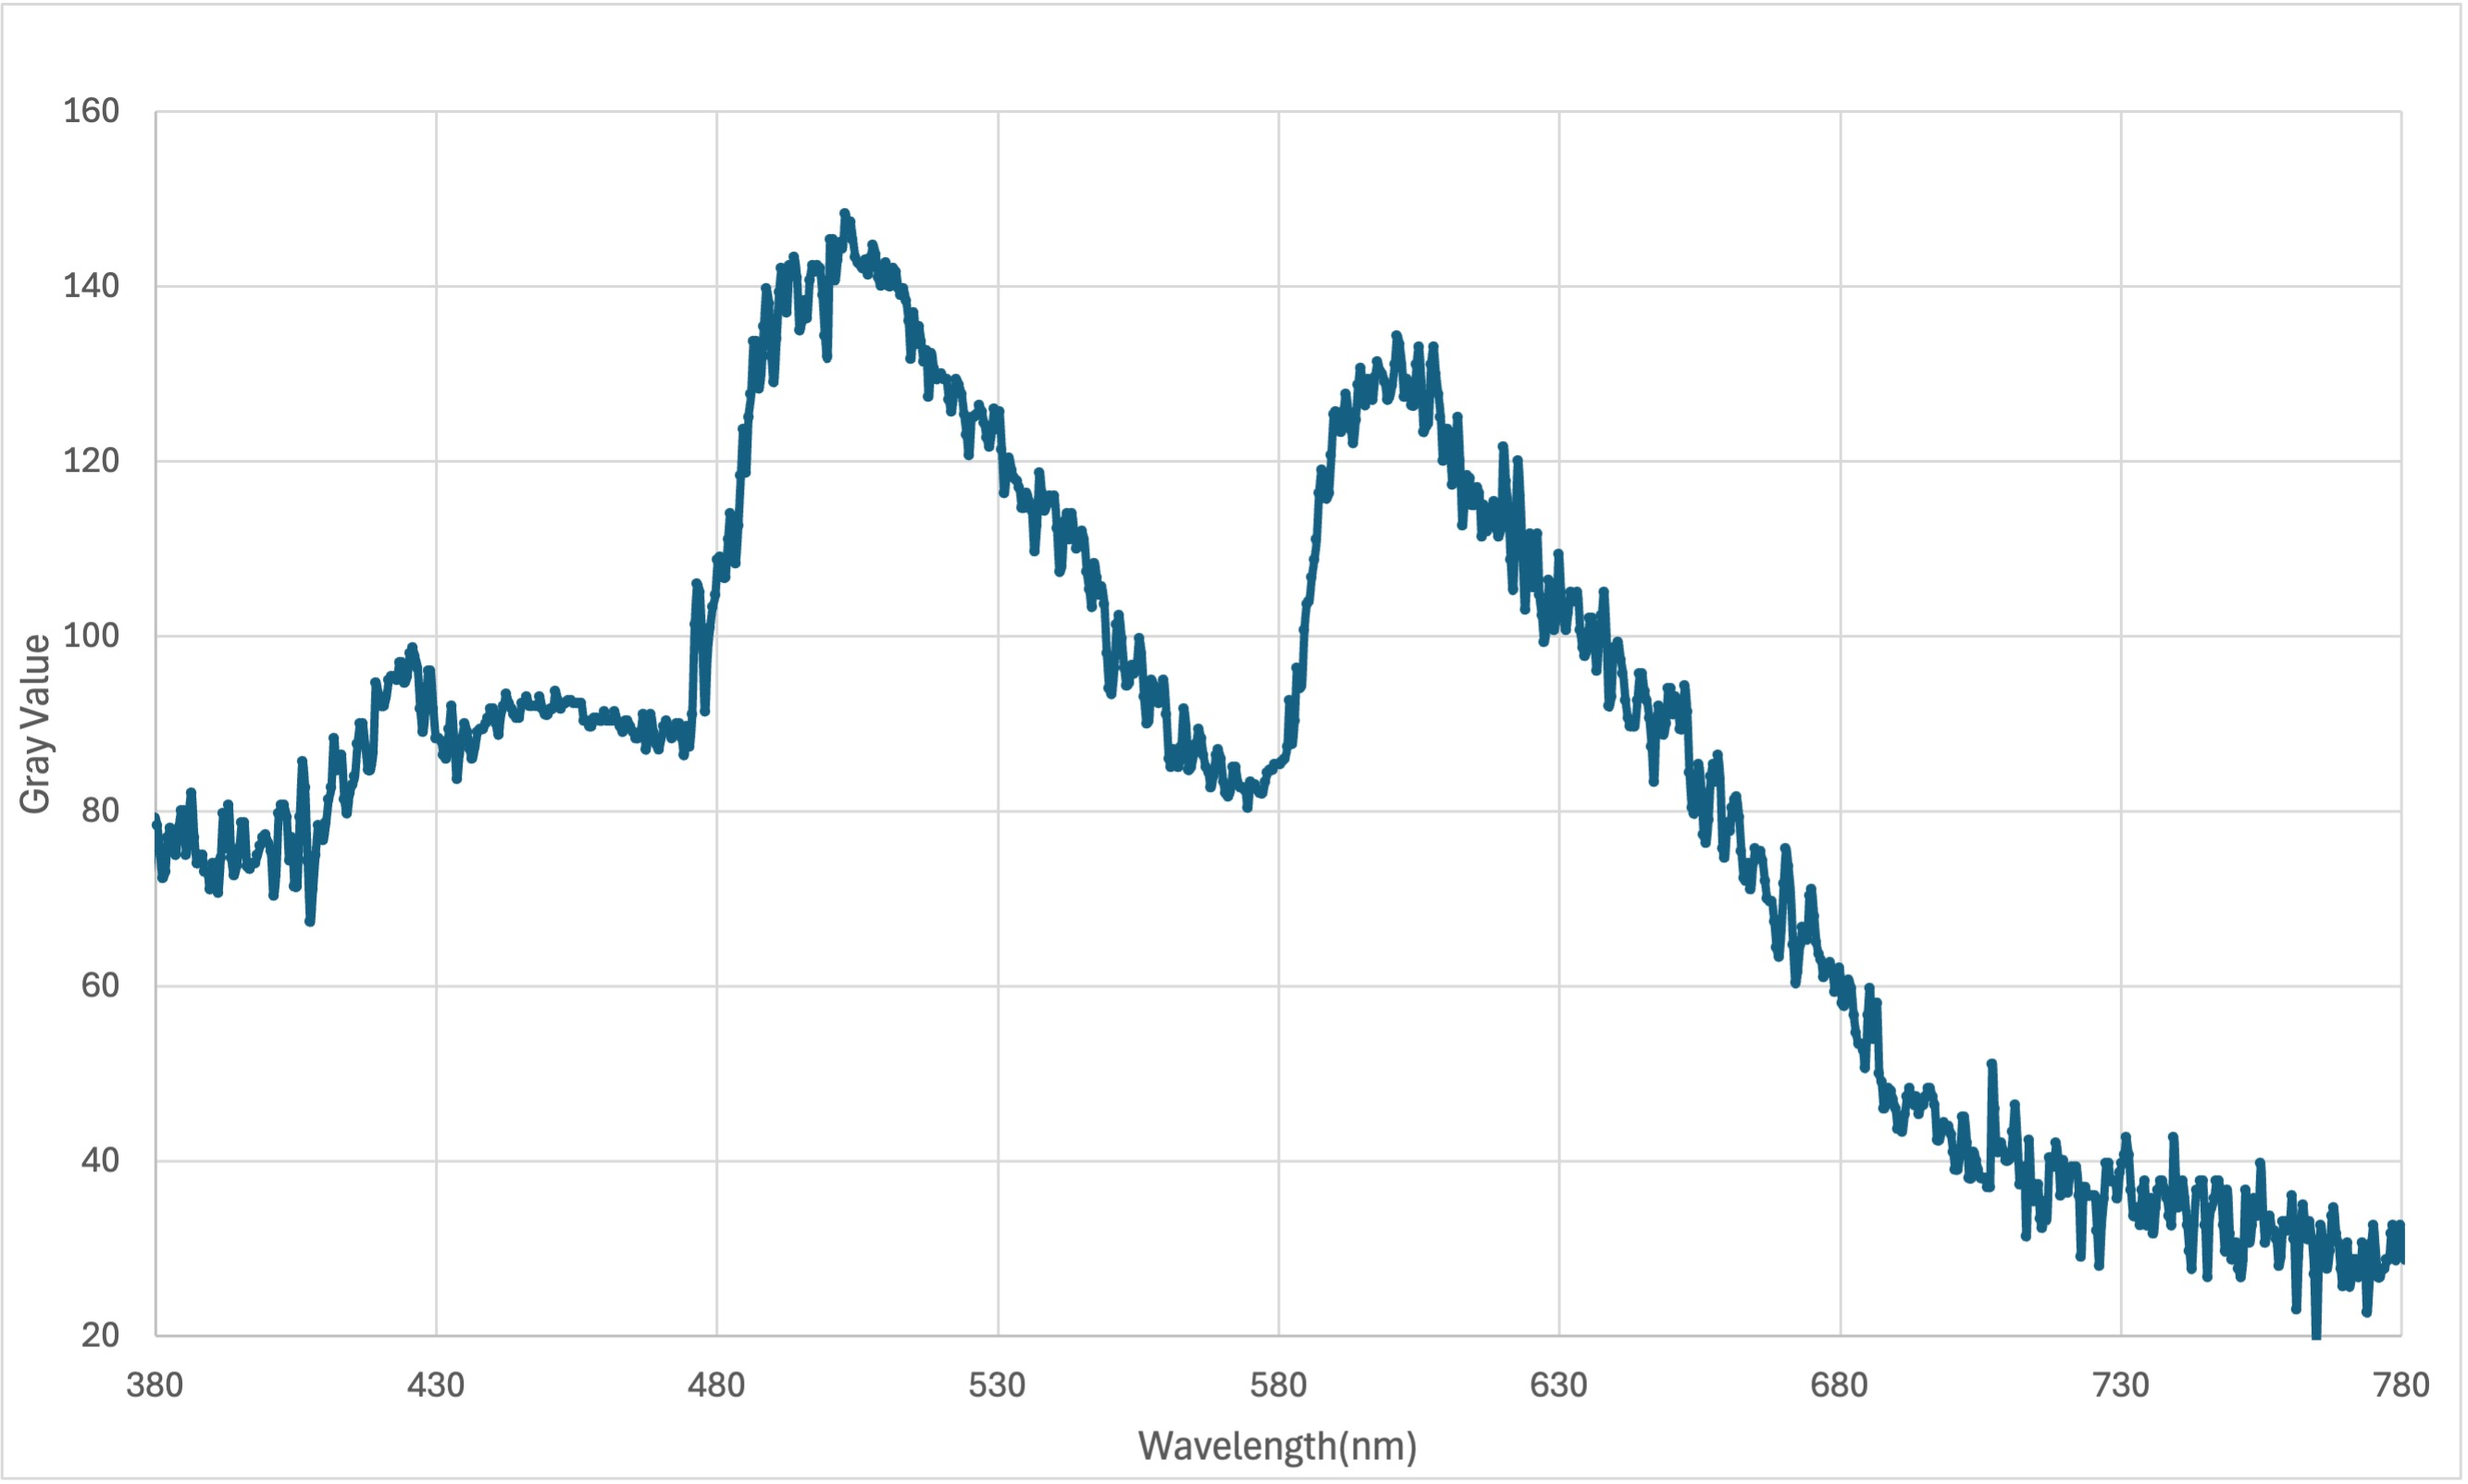
\includegraphics[width=\textwidth]{Sunlight_S.jpg}
            \end{minipage}
            }
            \caption{太阳光}
        \end{figure}

        \begin{figure}[H]
            \centering
            \scalebox{0.85}{
            \begin{minipage}{0.45\textwidth}
                \centering
                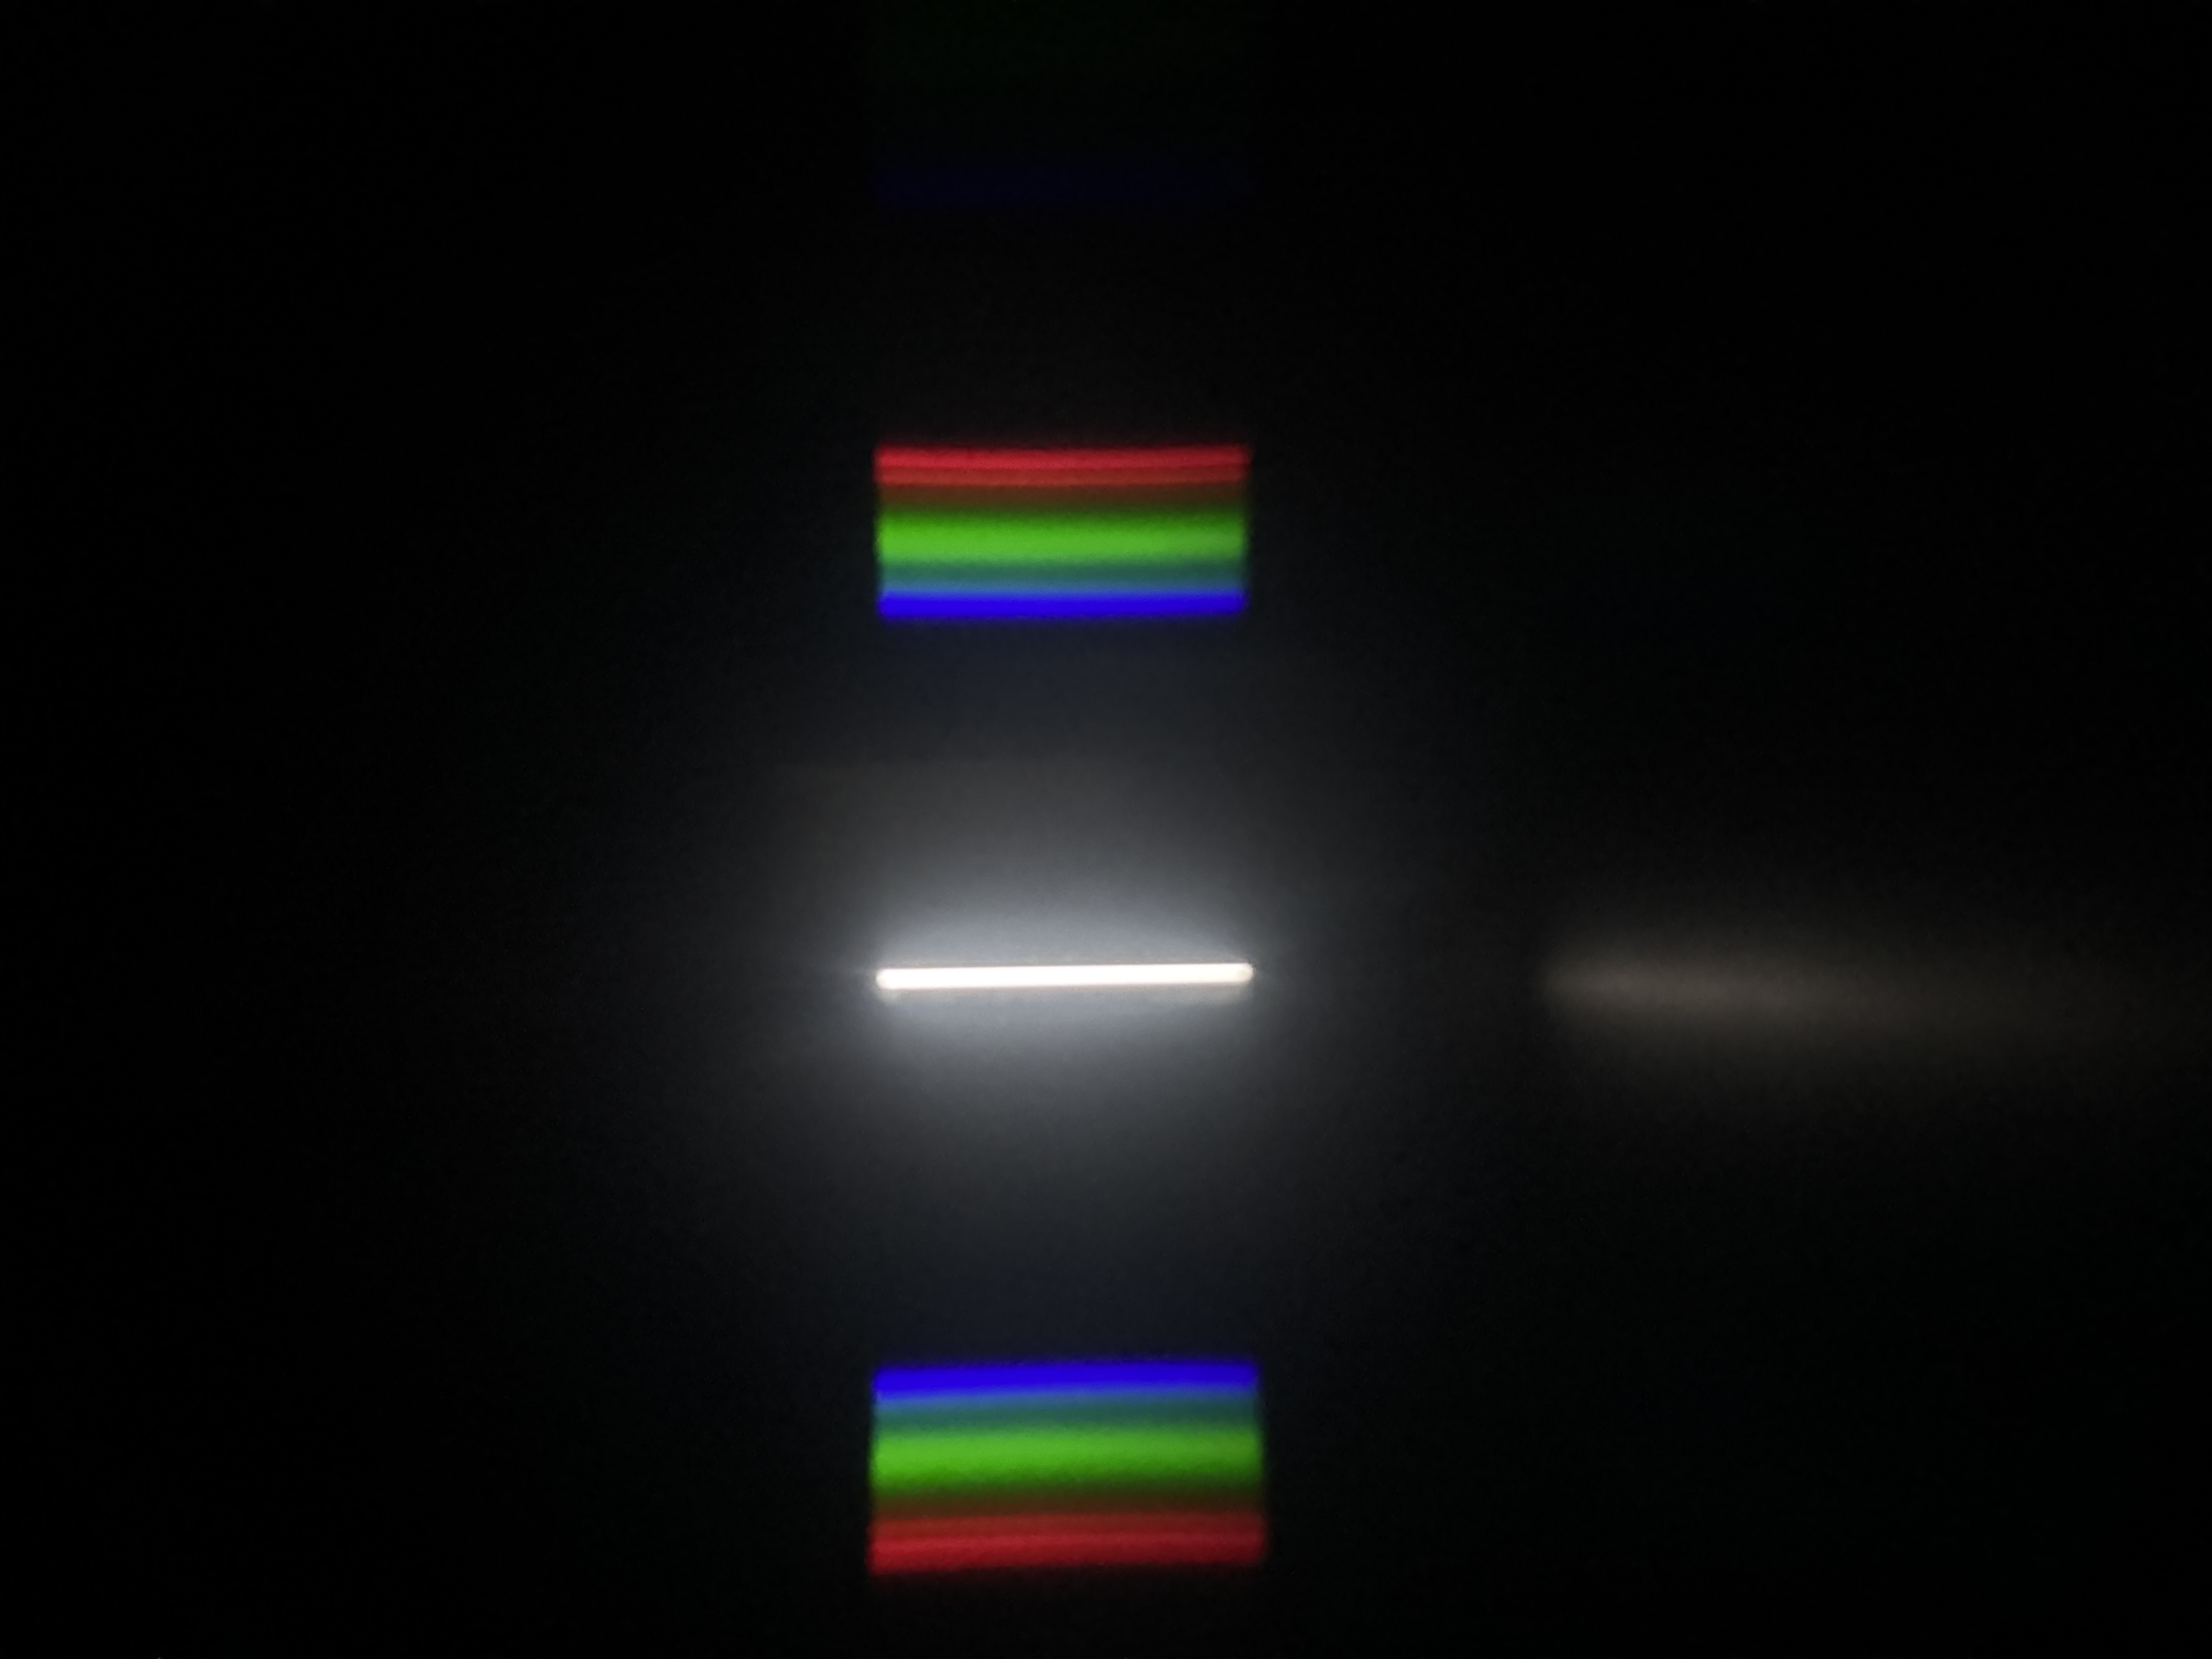
\includegraphics[width=\textwidth]{RGB Screen.JPG}
            \end{minipage}
            \begin{minipage}{0.45\textwidth}
                \centering
                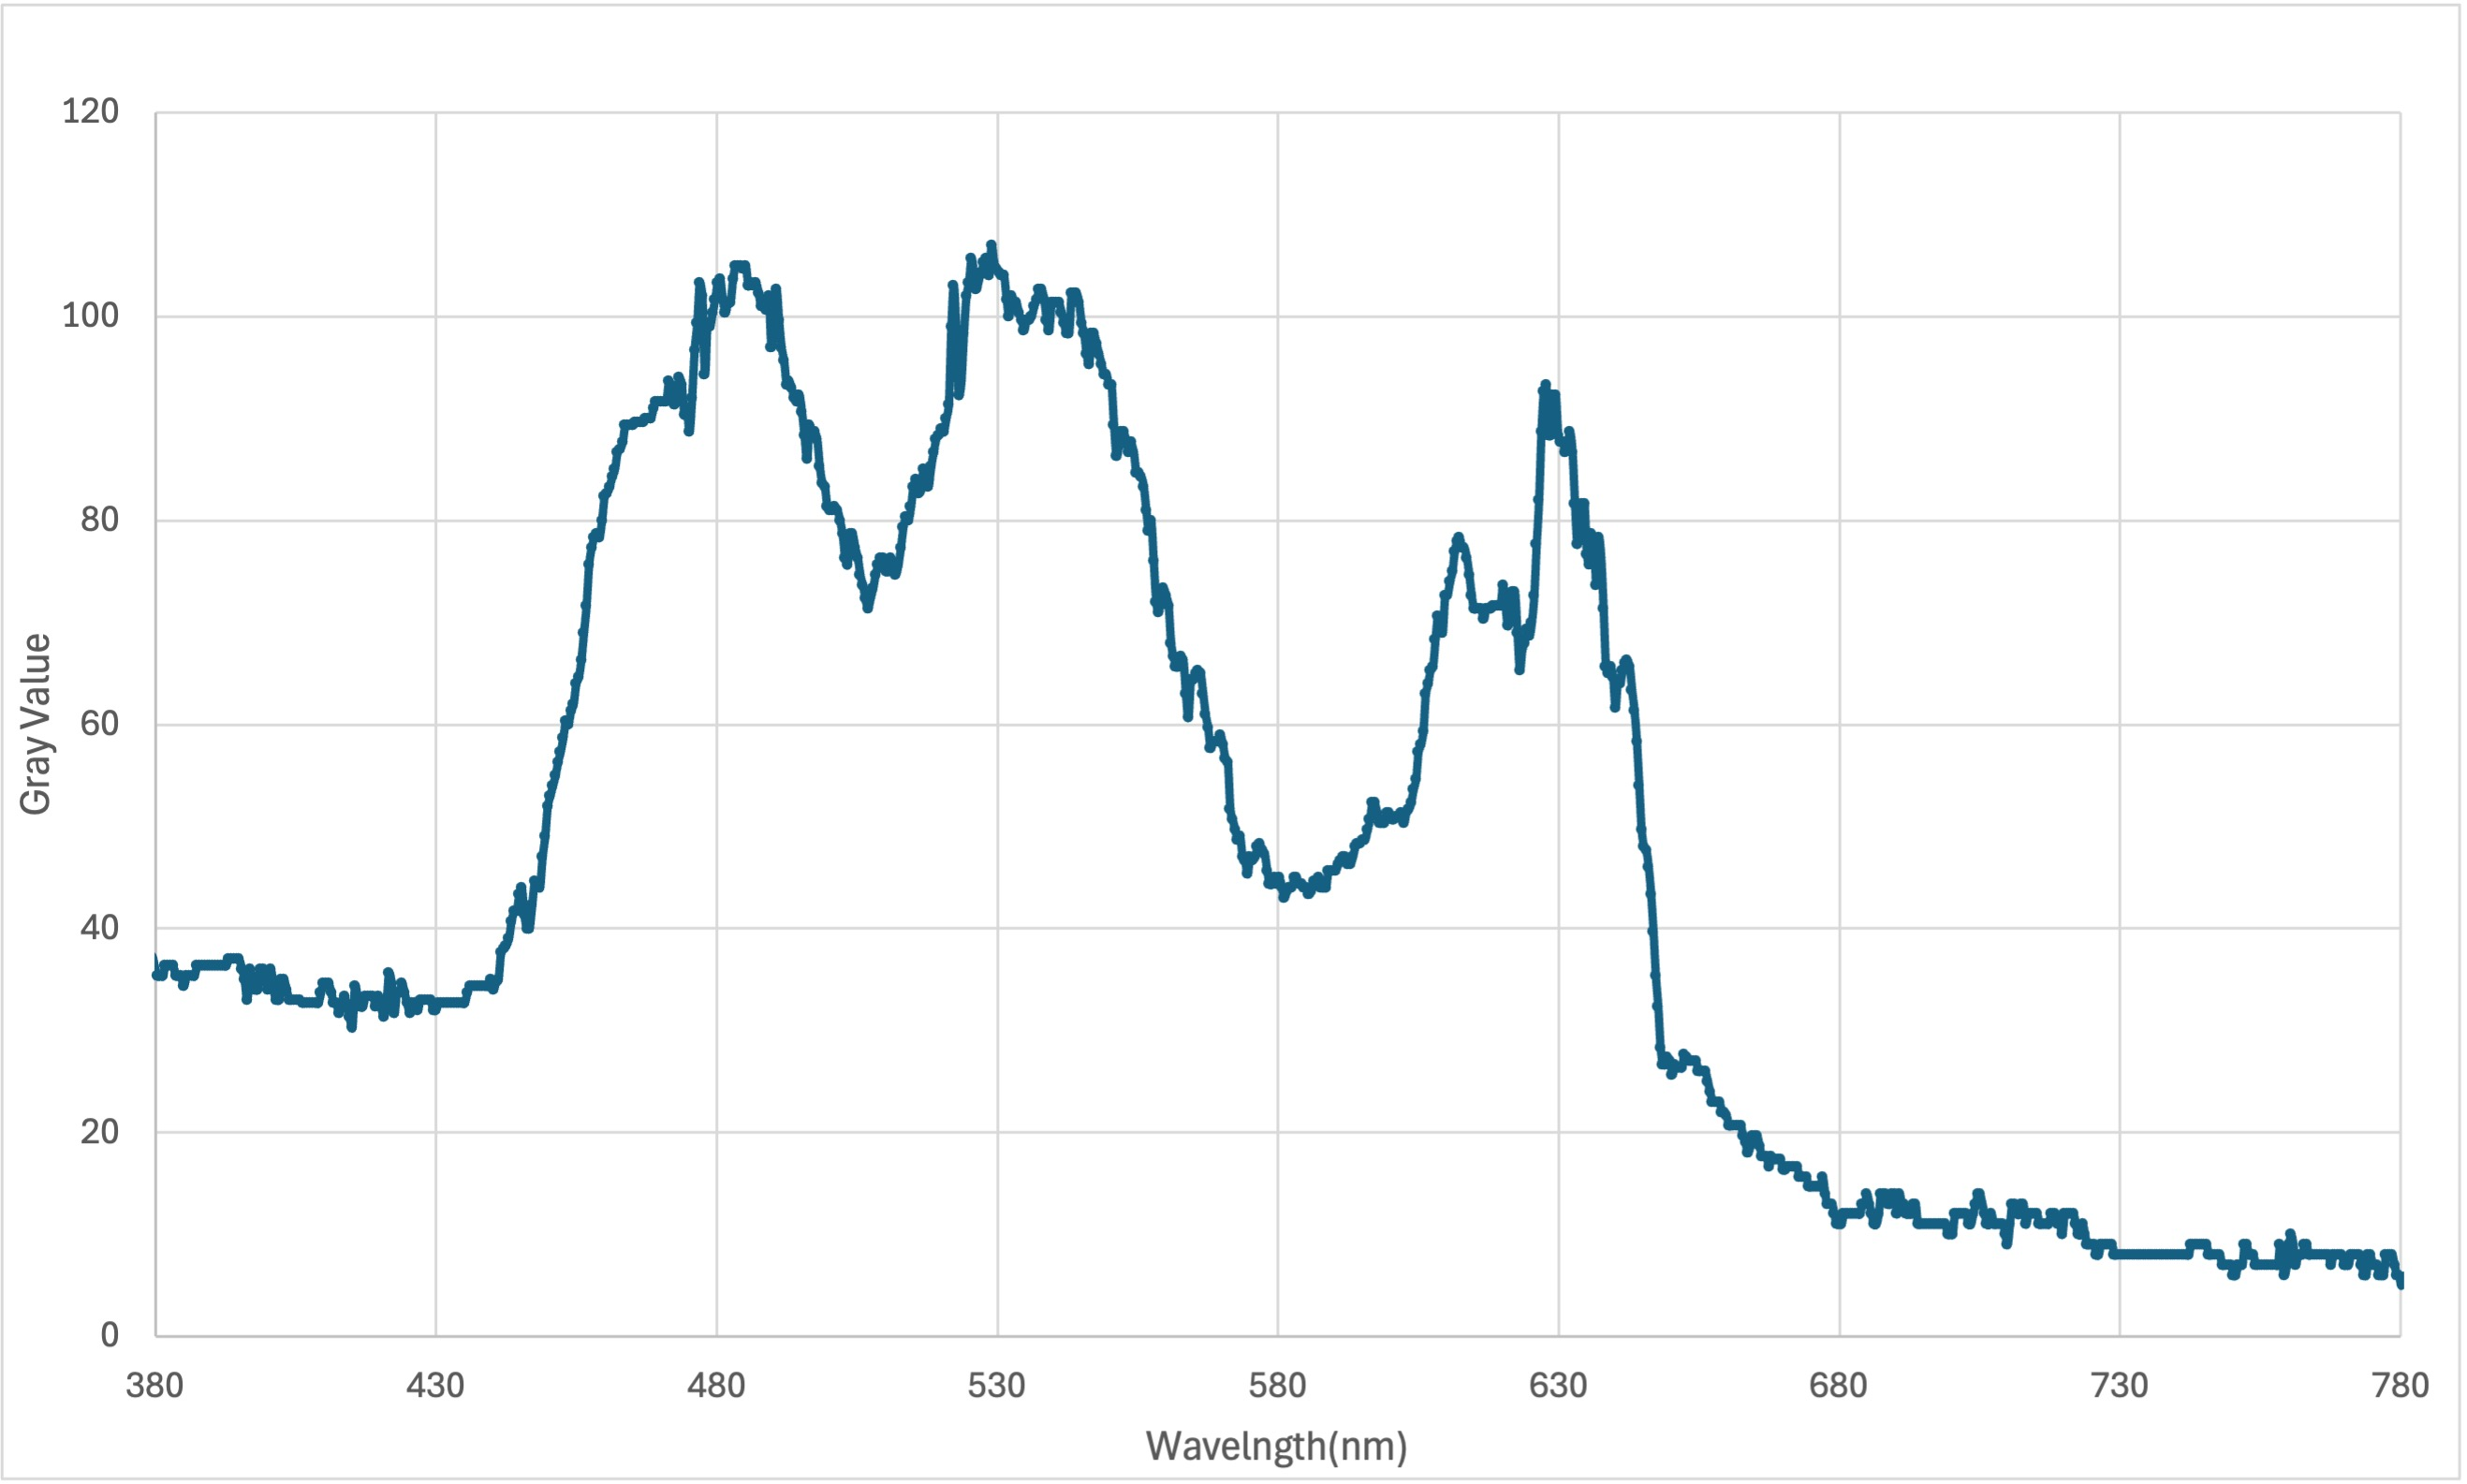
\includegraphics[width=\textwidth]{RGB Screen_S.jpg}
            \end{minipage}
            }
            \caption{RGB电脑屏幕}
        \end{figure}

        \item 误差分析
        \\[2.5mm]
        本实验的误差主要来源于以下几个方面：实验中制作的狭缝至光栅的距离有限，只能近似认为入射光是平行光线；光栅本身不平整，影响了产生的衍射图案；手机感光元件性能与人眼有差距，观察到手机拍摄图像红色区域偏暗、蓝色区域偏亮；采用前述方法确定波长标度时未考虑到拍摄视角导致的图像畸变，波长与距离关系式本身存在误差。
    \end{enumerate}
    



\end{enumerate}
\end{document}